\documentclass[11pt]{article}
\pdfinfoomitdate=1
\pdftrailerid{}
\pdfsuppressptexinfo=15
\usepackage[T1]{fontenc}
\usepackage{lmodern}
\usepackage{amsmath,amssymb,amsthm,mathtools,mathrsfs}
\numberwithin{equation}{section}
\usepackage[papersize={8.5in,11in},textwidth=6in,textheight=8in,centering]{geometry}
\usepackage[expansion=false]{microtype}
\usepackage{booktabs,array,enumitem,xcolor}
\usepackage{tikz}
\usetikzlibrary{arrows.meta,decorations.pathreplacing}
\usepackage[hidelinks]{hyperref}
\newcommand{\paperauthorname}{Haibo Lu}
\newcommand{\paperaffiliation}{Shanghai Institute of Technology, Shanghai 201418, People's Republic of China}
\newcommand{\paperemail}{luhaibo1985@gmail.com}
\newcommand{\paperorcid}{0009-0000-2717-5968}
\newcommand{\paperauthorblock}{%
  \paperauthorname\\
  {\small \paperaffiliation}\\
  {\small \href{mailto:\paperemail}{\texttt{\paperemail}}\quad
  \href{https://orcid.org/\paperorcid}{ORCID: \paperorcid}}%
}
\newcommand{\paperrunninghead}{Path selection in a Painleve oscillator}

\hypersetup{pdfauthor={Haibo Lu}}
\newtheorem{theorem}{Theorem}[section]
\newtheorem{proposition}[theorem]{Proposition}
\newtheorem{lemma}[theorem]{Lemma}
\newtheorem{corollary}[theorem]{Corollary}
\newtheorem{claim}[theorem]{Claim}
\theoremstyle{definition}
\newtheorem{definition}[theorem]{Definition}
\newtheorem{hypothesis}[theorem]{Hypothesis}
\theoremstyle{remark}
\newtheorem{remark}[theorem]{Remark}
\newcommand{\eps}{\varepsilon}
\newcommand{\R}{\mathbb R}
\newcommand{\Pcal}{\mathcal P}
\newcommand{\Kcal}{\mathcal K}
\newcommand{\Fcal}{\mathcal F}
\newcommand{\Tcal}{\mathcal T}
\newcommand{\Wcal}{\mathcal W}
\newcommand{\Ccal}{\mathcal C}
\newcommand{\dd}{\,\mathrm d}
\newcommand{\TD}{\mathrm{TD}}
\newcommand{\LO}{\mathrm{LO}}
\newcommand{\Acc}{\operatorname*{Acc}}
\newcolumntype{L}[1]{>{\raggedright\arraybackslash}p{#1}}
\setlength{\emergencystretch}{2em}
\newcommand{\reservestatementspace}{%
  \par\ifdim\dimexpr\pagegoal-\pagetotal\relax<8\baselineskip
  \newpage\fi}
\renewcommand{\figurename}{Fig.}

\newcommand{\Lip}{\operatorname{Lip}}
\newcommand{\cX}{\mathfrak X}
\newcommand{\X}{\mathfrak X}
\newcommand{\cC}{\mathcal C}
\newcommand{\cW}{\mathcal W}
\newcommand{\dF}{d_{\mathrm F}}
\newcommand{\cE}{\mathcal E}
\newcommand{\cP}{\mathcal P}
\newcommand{\cT}{\mathcal T}
\newcommand{\dH}{d_{\mathrm H}}
\newcommand{\cQ}{\mathcal Q}
\newcommand{\Clust}{\operatorname{Clust}}
\newcommand{\XiState}{\mathfrak X}

\hypersetup{pdftitle={Common free-flight selection and contact-phase sensitivity in a compliant Painleve oscillator},
 pdfsubject={Complete stopped paths, common selection and residual entrance phase}}
\title{Common free-flight selection and contact-phase sensitivity\\
in a compliant Painlev\'e oscillator}
\author{\paperauthorblock}
\date{}
\begin{document}
\maketitle
\begingroup
\renewcommand{\thefootnote}{}%
\begin{NoHyper}%
\footnotetext{Running head: \paperrunninghead.}%
\end{NoHyper}%
\endgroup
\begin{abstract}
We study the stiff limit of a compliant Painlev\'e oscillator with
relaxing normal memory, smooth friction and square-root belt-speed
detuning. From prescribed physical initial data to the first crossing
of a fixed nearby angle section, we classify and realize all limiting
ordered paths, including their infinite contact--flight cascades.
For fixed mechanical parameters, the outgoing family is common to the
prescribed compact parameter and preparation classes. Every free-flight
target is selected by one compliance sequence uniformly across those
classes, with each incoming datum retaining its own incoming arc.
First-angle contact selection obeys an entrance-constant law.
Unequal constants exclude common interior contact selection, even at
different contact phases. Along a sequence selecting an interior
contact target, smaller and larger entrance constants instead select
admission and release, respectively. Explicit threshold sequences
realize this ordering, which we establish for belt coefficients and
for locally constructed friction-profile curves.
The mechanism is a separation of scales: repeated return contraction
leaves an entrance-phase difference of order $1/\log(1/\eps)$, while
an actual contact stop requires a touchdown window of order $\eps$.
A complete-state comparison from the physical preparation preserves
the accuracy needed to distinguish them. This obstruction concerns first-angle stopping: a fixed
local observation patch crossed strictly at a prescribed interior
point instead permits common selection of that prefix.
\end{abstract}

\section{Introduction}
\label{sec:introduction}

A rigid frictional system can lose forward uniqueness at a Painlev\'e
singularity. Compliance restores an ordinary evolution, but its
vanishing limit need not select a single outgoing motion. We study
a compliant, smooth-friction unfolding of the critical oscillator
of Nordmark, V\'arkonyi and Champneys~\cite[Section~6.1]{NVC2018}.
Two masses are joined by a rigid link, with the lower mass contacting
a moving belt. Successive contacts and flights form a cascade whose
number of returns tends to infinity as compliance vanishes.

Our question concerns two different forms of independence from the
auxiliary contact parameters. Do they give the same family of limiting
paths? Can one sequence of compliances select the same member of that
family for all parameter values? We answer both questions for paths
stopped at the first crossing of a fixed nearby link angle. The system
has relaxing normal memory and friction smoothed at slip scale $\eps$,
with belt speed $U_b=U_*-k\sqrt\eps$ and fixed $k>0$.
Section~\ref{sec:model} specifies the compact mechanical, profile and
physical-preparation classes used throughout.

\paragraph{Earlier work and the present problem.}
Champneys and V\'arkonyi~\cite[Sections~4, 5.1 and~5.3]{CV2016}
place contact regularization, dynamic jam and reverse chatter within
the forward-continuation problem for frictional rigid bodies.
Compliance-dependent continuation already appears in reverse
chatter: Nordmark, Dankowicz and
Champneys~\cite[Sections~5.2 and~6.1]{NDC2009} give an asymptotic
matching argument for selecting different forward motions along
different compliance sequences, with numerical terminal curves for
a conservative normal law and Coulomb friction. The relaxing
normal law used here was introduced by Nordmark, V\'arkonyi and
Champneys~\cite[Equations~(20)--(21)]{NVC2018} in their study of
dynamic jam. The concluding discussion of their 2017 preprint
identifies motion beyond the first lift-off or the onset of impact
without collision as a further problem, including repeated
contacts. We determine that subsequent local motion under the
smooth friction and belt scaling fixed below, including every
stopped path and the common-sequence question.

Rigorous passage results in related contact problems resolve
several of the local difficulties. Hogan and
Kristiansen~\cite[Theorems~3.1--3.2]{HK2017} prove compression,
slip arrest and lift-off for a single impact without collision,
and a threshold separating it from immediate lift-off, at a fixed
negative Painlev\'e coefficient. Kristiansen and
Hogan~\cite[Theorem~6]{KH2018} prove persistence of a strong
canard at the degenerate point, using a second blow-up to resolve
the ellipticity left by the first. Their
erratum~\cite{KH2018Erratum} requires sufficiently small initial
tangential velocity for rigid-model slip arrest before the singular
point; the canard theorem is unchanged. The additional tasks here
are preparation of the independent normal memory into a repeatable
return domain, comparison through a growing number of returns,
and actual realization of every stopped contact prefix.

Regularization can also select one outgoing orbit in other
nonsmooth systems. For a truncated visible--invisible two-fold
normal form, Kristiansen and Hogan~\cite[Theorem~1]{KH2019TwoFold}
prove uniform contraction of a transverse incoming family towards
one outgoing orbit under arctangent regularization, with a
nonresonance condition and separation from the weak canard;
their Section~5 discusses other regularization functions.
In three-dimensional contact mechanics, Cheesman, Hogan and
Kristiansen~\cite[Sections~4--5]{CHK2023} use normal compliance
and a separate smoothing of spatial Coulomb friction to analyse
impact without collision. They resolve local sticking dynamics
and identify a Painlev\'e-I equation in the transition from
slipping to inconsistency.

For homogeneous singular ODEs, Drivas and
Mailybaev~\cite[Theorem~5 and Corollary~2]{DM2018} study expelling
regularizations approaching an exponentially attracting
renormalized cycle with positive mean radial drift.
Regularizations escaping into the basin of the same cycle share
a phase family of limiting continuations. Their geometric sequence
$\nu_n=\exp\{-T\langle F_r\rangle n+\chi\}$ selects phase
$\zeta=c-\chi$, with regularization-dependent $c$.
This gives a related distinction between a common limiting family
and a common selecting sequence. In the contact problem here, an
entrance-phase difference disappears at a free target but remains
larger than the fixed-angle contact stopping window. Selection
therefore depends on the target type, and the order of the entrance
constants determines the endpoint limits.

The scalar phase of a power-like return has a classical precedent.
Goncharuk and Kudryashov~\cite[Lemmas~5--6]{GK2019} prove
rectification and refined double-logarithmic parameter asymptotics,
following root estimates of Ilyashenko, Kudryashov and
Schurov~\cite[Sections~4.5--4.6]{IKS2018} and the smooth saddle-loop
work of Dumortier and Roussarie~\cite{DR1990}. We construct the
phase together with the complete mechanical graph and control its
accuracy along actual returns. Bressan and
Mazzola~\cite[Theorem~2]{BM2013} prove time--state graph convergence
for specified approximations of impulsive feedbacks. Here the
contact curves and their ordering are derived from the compliant
force law.

\paragraph{Main conclusions.}
Theorem~\ref{thm:whole} classifies and realizes every stopped-path
limit from the prescribed initial data. Each path consists of its
incoming rigid arc, an infinite ordered contact--flight cascade
leaving the singular point, and a terminal contact or flight prefix.
At fixed mechanical parameters and observation section, the outgoing
family is common to the prescribed auxiliary classes; different
incoming data retain their own incoming arcs.
Theorem~\ref{thm:common-free} gives the stronger common-sequence
conclusion for every free-flight target, uniformly over those compact
classes.

Theorem~\ref{thm:contact-selection} states the entrance-constant law
for contact targets within the same physical model and classes.
Two fixed unequal constants exclude common interior contact selection,
even at different contact phases. Moreover, on any sequence selecting
an interior contact target for one datum, smaller and larger entrance
constants force admission and release for the other data.
Proposition~\ref{sel:threshold-selection} gives explicit threshold
sequences and uniform endpoint selection on compact subclasses
separated from the threshold. Equal constants are necessary for
common interior selection; these estimates do not make them
sufficient. The belt application is
Corollary~\ref{cor:belt-contact-selection};
Corollary~\ref{cor:friction-profile-selection} gives the corresponding
application along an admissible friction-profile curve constructed
locally through each baseline profile.

\paragraph{Mechanism.}
Recurring compression consumes tangential slip; arrest changes the
normal response, and the inherited compression drives release.
The subsequent cubic free-flight balance gives a return scale
of order $\delta^{3/4}$. On the invariant graph of the complete
normalized limiting return, the exact base map and its phase satisfy
\[
 F_\lambda(\delta)\sim K_\lambda\delta^{3/4},\qquad
 \mathcal S_\lambda(F_\lambda(\delta))
       =\tfrac34\mathcal S_\lambda(\delta).
\]
The prescribed physical preparation determines a bounded entrance
correction. Repeated return contraction reduces the difference of
two such corrections to order $1/\log(1/\eps)$ at a fixed positive
section. An actual contact stop at $p=-as$ requires the much narrower
window $\delta=s+O_s(\eps)$. Thus
\[
 \eps\ll\frac1{\log(1/\eps)}\ll1.
\]
The same entrance difference vanishes in the free-target limit but
still separates the contact stopping windows and orders their
endpoint limits. The comparison uses the exact phase at the fixed
section, not just its leading logarithmic approximation.

\paragraph{Proof route.}
Section~\ref{sec:local-results} derives the complete prepared entrance
and the repeatable local return from the physical initial data.
Section~\ref{sec:graph} constructs the exact graph and compares the
actual full states through the required event indices.
Section~\ref{sec:physical-paths} pairs whole returns and scans a
fixed actual contact index to classify and realize complete paths.
Section~\ref{sec:contact-selection} compares the residual phase with
the contact window and proves the belt and profile applications;
Section~\ref{sec:observations} treats longer paths, first-angle
truncation and strict local crossings. The local estimates and
cancellations remain in the appendices.

\section{The physical model and prescribed initial data}
\label{sec:model}

\subsection{An independent belt parameter}
The oscillator consists of two point masses joined by a rigid link.
The upper mass moves vertically against a spring and damper; the lower
mass can contact a belt moving to the left. In the nondimensional
coordinates of \cite[Section~6.1]{NVC2018}, both masses and the link
length are one. The link angle $\phi$ is measured from the downward
vertical, and the upper mass is at height $1+\psi$ above the undeformed
belt. A torsional spring acts on $\phi$. The observables $y$ and $u$
below are the lower mass's height and its slip relative to the belt.
Let $q=(\phi,\psi)^T$, $\omega=\dot\phi$, and define
\begin{equation}
 y=\psi+1-\cos\phi,\qquad v=\dot y,
 \qquad u=\omega\cos\phi+U_b,\qquad U_b=3/5+\eta.
 \label{eq:bd-observables}
\end{equation}
The belt detuning $\eta$ is independent of the mechanical parameters.
We use the critical mechanical family of \cite[Section~6]{NVC2018}:
\begin{gather}
 M(\phi)\ddot q=f_{\beta,\kappa}(q,\dot q)
                  +Q_N(\phi)\lambda_N+Q_T(\phi)\lambda_T,
 \label{eq:bd-mechanics}\\
 M=\begin{pmatrix}1&\sin\phi\\\sin\phi&2\end{pmatrix},
 \quad Q_N=\binom{\sin\phi}{1},\quad Q_T=\binom{\cos\phi}{0},
 \nonumber\\
 f_{\beta,\kappa}=
 \binom{-(\phi-\phi_0)-\sin\phi}
       {-\kappa\psi-c_\psi\dot\psi-2-\cos\phi\,\omega^2},
 \nonumber\\
 \mu=25/12,\quad c_\psi=25(18-7\beta)/108,
 \quad\phi_0=\phi^*+49/20-7\beta/12-9\kappa/50,
 \nonumber\\
 \quad (\cos\phi^*,\sin\phi^*)=(3/5,4/5).
 \label{eq:bd-critical-family}
\end{gather}
The prescribed completion is
\begin{equation}
 \eps\dot z=-z-\eps^2\lambda_N,\qquad
 \lambda_N=\eps^{-2}(z-y)_+,\qquad
 \lambda_T=-\mu\Phi_\theta(u/\eps)\lambda_N.
 \label{eq:bd-completion}
\end{equation}
Thus contact is determined by $g=y-z$, not by $y$ alone.
In flight $z(t)=z_r e^{-(t-t_r)/\eps}$, and
$\dot g=v+z/\eps$ at release. Every release below is the first
zero of the active normal force on the stated continuous contact
passage, and every touchdown is the first zero of the subsequent
positive free gap. Initial capture may contain other contacts.

Write $X=(\phi,y,\omega,v)$ and eliminate
$\psi=y-1+\cos\phi$, $\dot\psi=v-\sin\phi\,\omega$.
The free mechanical vector field and saturated contact field per unit
normal force are
\begin{equation}
 F_{\rm free}=(\omega,v,(M^{-1}f)_1,b),\qquad
 Q_{\rm sat}=(0,0,(M^{-1}(Q_N-\mu Q_T))_1,p),
 \label{eq:bd-fields}
\end{equation}
where
\begin{equation}
 b=Q_N^TM^{-1}f+\cos\phi\,\omega^2,\qquad
 a_T=Q_T^TM^{-1}f-\sin\phi\,\omega^2,
 \qquad p=C-\mu B.
 \label{eq:bd-free-accelerations}
\end{equation}
The exact contact equations for the observables are
\begin{equation}
 \dot v=b+(C-\mu B\Phi_\theta(u/\eps))\lambda_N,
 \qquad
 \dot u=a_T+(B-\mu A\Phi_\theta(u/\eps))\lambda_N.
 \label{eq:bd-contact-accelerations}
\end{equation}
Direct inversion of $M$ gives
\begin{equation}
 A=\frac{2\cos^2\phi}{1+\cos^2\phi},\qquad
 B=\frac{\sin\phi\cos\phi}{1+\cos^2\phi},\qquad
 C=\frac1{1+\cos^2\phi},\qquad
 D=C-B^2/A=\frac12.
 \label{eq:bd-delassus}
\end{equation}
In particular the coefficient after eliminating tangential force is
positive even when the saturated coefficient $p$ is zero or negative.
The chart is restricted throughout so that $\cos\phi$ has a common
positive lower bound.
Since $p=C(\phi)-\mu B(\phi)$, the rate
$p_\phi(G)=a$ below permits a further common restriction with
$p_\phi>0$. Each observation section $p=-as$ then fixes one angle
$\phi_s$ on this branch.

\subsection{Critical rates and the working box}
At $G=(\phi^*,0,-1,0)$ in the mechanical coordinates,
$p=b=0$ and the tuned slip is zero. The detuned slip at $G$ is
$\eta$. Substitution in \eqref{eq:bd-fields}--\eqref{eq:bd-delassus}
gives
\begin{gather}
 A_G=9/17,\quad B_G=6/17,\quad C_G=25/34,\quad
 h:=\mu A_G-B_G=3/4,\qquad a:=175/408,
 \nonumber\\
 F_{\rm free}p(G)=-a,\quad F_{\rm free}b(G)=-c_\lambda,
 \quad a_T(G)=d_\lambda,\quad Q_{\rm sat}b(G)=a\beta,
 \label{eq:bd-critical-rates}\\
 c_\lambda=\frac{126765+61425\beta-30625\beta^2
                    -(9450\beta+8262)\kappa}{55080},\qquad
 d_\lambda=\frac{495-175\beta-54\kappa}{180},
 \nonumber\\
 \ell:=\lambda_*=\frac{c_\lambda}{a(\beta-1)},\qquad
 g_*:=d_\lambda-h\ell
       =\frac{55825\beta+17712\kappa-213390}{31500(\beta-1)}.
 \label{eq:bd-incoming-rates}
\end{gather}
Here $\lambda=(\beta,\kappa)$; we also write $c=c_\lambda$
and $\gamma=-g_*>0$. These formulas can be checked by differentiating the
explicit fields in \eqref{eq:bd-fields}. At $G$ the added generalized
acceleration is $(-5/4,1)$ in $(\ddot\phi,\ddot\psi)$, so its
$(\dot\omega,\dot v)$ components are $(-5/4,0)$, and
\begin{equation}
 p_\phi(G)=a,\qquad
 \det D_{(\phi,\omega)}(p,b)(G)=-6125\beta/41616.
 \label{eq:bd-chart-determinant}
\end{equation}
Thus $(p,b,y,v)$ are analytic coordinates on a common neighborhood;
write $\Xi(p,b,y,v)$ for their inverse mechanical chart.

Fix a sufficiently small closed box $\Lambda$ about $(7/3,0)$ in
the half-plane $\kappa\ge0$, with
\begin{equation}
 2<\beta_-\le\beta\le\beta_+<5/2,
 \qquad c,d_\lambda,\ell,-g_*>0,
 \qquad |\det D_{(\phi,\omega)}(p,b)(G)|>0,
 \label{eq:bd-box}
\end{equation}
all with common strict margins. Uniform statements use this compact
box; its interior is relative to $\kappa\ge0$.
The upper bound $\beta_+<5/2$ records the scope of the present proof.
The coefficient $\beta$ is also the exponent in the incoming weak
trace, as the scalar equation in Section~\ref{sec:entry}
shows. We use the prescribed compact range \eqref{eq:bd-box} to
construct the weak curve and obtain the common forcing bound
\eqref{ent:forcing-domination} in the upstream normal-energy and
weak-transport estimates. The strict sign and chart margins fix the
event orientation and the common coordinate neighborhood.

\subsection{Profiles and physical preparation}
Let $\Theta$ be compact, and let $\theta\mapsto\Phi_\theta$ be
continuous in the metric
\begin{equation}
 d_{\bar\alpha}(\Phi,\Psi)=
 \max_{0\le j\le4}\sup_{q\in\R}
 e^{\bar\alpha|q|}|\partial_q^j(\Phi-\Psi)(q)|,
 \qquad 0<\alpha<\bar\alpha<2.
 \label{eq:bd-profile-metric}
\end{equation}
Its image is compact in the affine space consisting of $\tanh$ plus
functions with finite weighted norm. Fix a compact
$I_s=[s_-,s_+]\Subset(-1,1)$ containing $B/(\mu A)$ on the
working mechanical chart. The following bounds hold with common
constants $0<M_{\rm sl}<Q_\Phi$, $m_\Phi,\varkappa_{\rm sl},C_\Phi>0$:
\begin{enumerate}[label=\textup{(F\arabic*)}]
\item $\Phi_\theta$ is strictly increasing, $\Phi_\theta(0)=0$,
 has values in $(-1,1)$ and limits $\pm1$ at $\pm\infty$.
\item $\Phi_\theta([-Q_\Phi,Q_\Phi])\supset I_s$,
 $\Phi_\theta'\ge m_\Phi$ there, and its first four derivatives
 are uniformly bounded there.
\item $\Phi_\theta(M_{\rm sl})\ge s_++\varkappa_{\rm sl}$ and
 $\Phi_\theta(-M_{\rm sl})\le s_--\varkappa_{\rm sl}$.
\item For $q\ge M_{\rm sl}$,
 \[
 1-\Phi_\theta(q)+\sum_{j=1}^4q^j|\Phi_\theta^{(j)}(q)|
                 \le C_\Phi e^{-\alpha q},
 \]
 with the reflected bound on the negative tail.
\end{enumerate}
The slip threshold $M_{\rm sl}$ is fixed with the profile class and
mechanical chart.
Nonodd profiles are allowed. Each profile is fixed before taking
the stiff limit. The family $\tanh(\theta q)$, $1\le\theta\le5/4$,
is an example: all derivatives through order four are bounded by
$C(1+|q|^4)e^{-2|q|}$ on the tails, as are the label derivatives
up to an extra polynomial factor. This proves both (F4) and
continuity in \eqref{eq:bd-profile-metric}; monotonicity gives the
remaining conditions after the strip is chosen large enough.

Choose a small fixed $p_0>0$ and a continuous compact family of
saturated rigid data $(\phi_\nu,\omega_\nu)$ on $p=p_0$.
Their positive-slip rigid orbits reach $G$ and have traces
\begin{equation}
 b_{{\rm rig},\nu}(p)=\bar b_\lambda(p)+C_1(\lambda,\nu)p^\beta
                 +\mathcal R_C(p),\qquad
 |\partial_p^j\mathcal R_C(p)|\le Cp^{\beta+1-j},\quad 0\le j\le3,
 \label{eq:bd-prescribed-trace}
\end{equation}
where $\bar b_\lambda(p)=-\ell p+O(p^2)$ is the analytic weak
curve constructed in Section~\ref{sec:entry}.
On each closed rigid subarc before $G$, the force $-b/p$ and tuned
slip have common positive lower bounds. The rigid trace is unchanged
by detuning: $U_b$ enters only the slip observable and the profile.

For a fixed fast triple $\mathbf n=(Y_0,V_0,Z_0)$ in any prescribed
compact set, the complete physical initial state is
\begin{equation}
 \cX_\eps(0;\lambda,\theta,\nu,\mathbf n)
       =(\phi_\nu,\eps^2Y_0,\omega_\nu,\eps V_0,\eps^2Z_0)
 \label{eq:bd-physical-initial-data}
\end{equation}
in coordinates $(\phi,y,\omega,v,z)$.
The slow datum and fast triple stay fixed as $\eps$ varies.
The initial state need not be in contact. For $\mathbf n=0$ it is
the same full physical state for every compliance and profile.
No later release or touchdown state is independently prepared.
The class is nonempty: the analytic weak curve supplies a rigid
datum at $p_0$, and a compact interval of nearby weak coefficients
supplies more. The scalar construction in Section~\ref{sec:entry} gives
\eqref{eq:bd-prescribed-trace}. The positive limits of $-b/p$ and
$u_0/p$ then give the closed-arc margins after the chart is reduced.

\paragraph{Standing convention.}
Fix the compact profile and physical-preparation classes above and
$k\in I=[k_-,k_+]\Subset(0,\infty)$; the nominal mechanical box
may then be reduced jointly for these same classes. All error
estimates and event margins are uniform on the resulting compact
label classes. Unless explicitly stated otherwise, mechanical
parameters and each sufficiently small positive observation section
are fixed before $\eps\downarrow0$. The common graph, return and
section cutoffs are chosen once before these targets. Uniform
selection is asserted only where stated; each incoming datum keeps
its own prescribed rigid arc.

The complete label is $\mathfrak l=(\lambda,k,\theta,\nu,\mathbf n)$.
We use $\cX=(\phi,y,\omega,v,z)$ for the full physical state and
$X=(\phi,y,\omega,v)$ for its mechanical part. In a five-state norm,
$G$ includes its zero memory coordinate. Put
$r=k\sqrt\eps=-\eta$. The actual belt slip is
$u_r=u=\omega\cos\phi+U_*-r$; the critical-speed slip is
$u_0=\omega\cos\phi+U_*=u_r+r$.
The coefficient $k$ and $r$ remain constant along each trajectory;
the physical belt speed follows $U_b=U_*-k\sqrt\eps$ as compliance
varies. The slow datum and scaled fast triple $\mathbf n$ remain fixed;
the physical initial state follows \eqref{eq:bd-physical-initial-data}.

\section{Complete paths and their selection}
\label{sec:main-results}

We stop the original trajectory at its first crossing of one fixed
downstream section. The limiting object retains the incoming rigid
arc, every return in an accumulating cascade and the final contact
or flight prefix. Its contact pieces carry an order, although their
physical durations vanish.

\subsection{The curves and their topology}
For continuous oriented curves $f,g:[0,1]\to\R^5$, put
\begin{equation}
 \dF(f,g)=\inf_{h\in\mathrm{Homeo}_+([0,1])}
                 \sup_{q\in[0,1]}|f(h(q))-g(q)|.
 \label{eq:ps5-frechet}
\end{equation}
We identify curves at zero distance. Pauses and constant pieces are
therefore allowed. Equivalently, one can use two nondecreasing
continuous surjections in the comparison: approximate a surjection
$a$ by $(1-\eta)a+\eta\,\mathrm{id}$ and use uniform continuity,
then compose the resulting homeomorphisms. For compact path images,
\begin{equation}
 \dH(A,B)=\max\{\sup_{x\in A}\inf_{y\in B}|x-y|,
                    \sup_{y\in B}\inf_{x\in A}|x-y|\}
 \le\dF(f,g),\quad A=f([0,1]),\ B=g([0,1]).
 \label{eq:ps5-hausdorff}
\end{equation}

Write $I_{\lambda,\nu}$ for the prescribed saturated rigid incoming
arc from $(\phi_\nu,0,\omega_\nu,0,0)$ to $G$, oriented in physical
time. Appendix~\ref{sec:detuned-return} and Section~\ref{sec:graph} construct an
exact limiting graph return $F=F_\lambda$ and its ordered one-return
curve $\cC_{\lambda,d}:[0,3]\to\R^5$. The three parameter intervals
describe saturated compression, inherited normal release and the
following first free flight: $\alpha=0,1,2,3$ mark touchdown, slip
arrest, release and the next touchdown, respectively.
These are finite-scale curves, retaining
their exact $\sqrt d$ dependence. They satisfy
\begin{equation}
 \cC_{\lambda,d}(3)=\cC_{\lambda,F(d)}(0),\qquad
 \sup_{0\le\alpha\le3}|\cC_{\lambda,d}(\alpha)-G|
                      \le C d^{3/4}.
 \label{eq:ps5-joins}
\end{equation}
On contact $p(\cC_{\lambda,d}(\alpha))=-ad$; on the free part it
strictly decreases from $-ad$ to $-aF(d)$. For fixed sufficiently
small $s>0$, set $d_*=F^{-1}(s)$. There is consequently a unique
continuous free-section parameter $j_s:[d_*,s]\to[2,3]$ with
\begin{equation}
 p(\cC_{\lambda,d}(j_s(d)))=-as,\qquad
 j_s(d_*)=3,\quad j_s(s)=2.
 \label{eq:path-free-section}
\end{equation}
The possible terminal data form the compact set
\begin{equation}
 \mathcal A_s=\{(d,j_s(d)):d_*\le d\le s\}
                       \cup(\{s\}\times[0,2]).
 \label{eq:ps5-domain}
\end{equation}
Its graph branch records free-flight stopping; the vertical segment
records contact stopping.

For $d\in[d_*,s]$, let $b_m=F^{-m}(d)$, $m\ge0$. These bases tend
to zero. Define $L_d(0)=G$ and trace $\cC_{\lambda,b_m}$ linearly on
$[2^{-m},2^{-(m-1)}]$ for $m\ge1$. The joins and bound in
\eqref{eq:ps5-joins} give a continuous curve. The complete curves are
\begin{equation}
 \cW_{\lambda,\nu,s}(d,\alpha)
   =I_{\lambda,\nu}\star L_d\star
                   \cC_{\lambda,d}|_{[0,\alpha]},
       \qquad(d,\alpha)\in\mathcal A_s.
 \label{eq:ps5-whole}
\end{equation}
Here $\star$ preserves order and joins equal endpoints. One may assign
one third of $[0,1]$ to each factor; a zero final prefix is constant.
Its compact image is
\begin{equation}
 W_{\lambda,\nu,s}(d,\alpha)
  =I_{\lambda,\nu}([0,1])\cup\{G\}
    \cup\bigcup_{m\ge1}\cC_{\lambda,b_m}([0,3])
    \cup\cC_{\lambda,d}([0,\alpha]).
 \label{eq:ps5-whole-image}
\end{equation}
The parameter $\alpha$ records the order along each completed contact
and free return.
At admission the two terminal pairs represent one ordered path:
$\cW_{\lambda,\nu,s}(d_*,3)=\cW_{\lambda,\nu,s}(s,0)$.
Indeed, $F(d_*)=s$ identifies the final full return of the former
with the last return already contained in $L_s$. Their parameter
pairs remain distinct. Figure~\ref{fig:ordered-stopped-path} shows
the order and terminal domain.
% MIXED: exact labels and joins, schematic widths and free-graph shape.
% The upper strip is an order diagram, not a coordinate projection or clock.
\begin{figure}[!htbp]
\centering
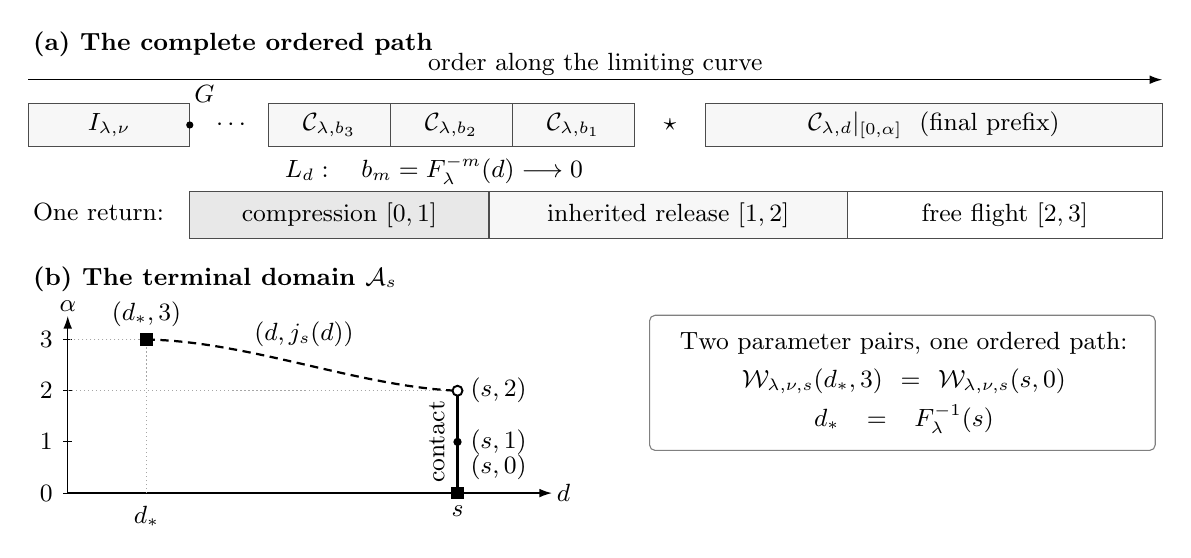
\begin{tikzpicture}[
 x=1cm,y=1cm,font=\small,
 every node/.style={inner sep=1.5pt},
 box/.style={draw=black!70,line width=.5pt,fill=black!3},
 arrow/.style={-{Latex[length=1.6mm,width=1.1mm]},line width=.5pt},
 guide/.style={draw=black!35,densely dotted,line width=.45pt}
]
 \node[anchor=west,font=\small\bfseries] at (0,5.75)
   {(a) The complete ordered path};
 \draw[arrow] (0,5.30) -- (14.4,5.30)
   node[midway,above] {order along the limiting curve};
 \draw[box] (0,4.45) rectangle (2.05,5.00);
 \node at (1.025,4.725) {$I_{\lambda,\nu}$};
 \fill (2.05,4.725) circle[radius=1.3pt];
 \node[above right] at (2.05,4.95) {$G$};
 \node at (2.60,4.725) {$\cdots$};
 \draw[box] (3.05,4.45) rectangle (4.60,5.00);
 \draw[box] (4.60,4.45) rectangle (6.15,5.00);
 \draw[box] (6.15,4.45) rectangle (7.70,5.00);
 \node at (3.825,4.725) {$\mathcal C_{\lambda,b_3}$};
 \node at (5.375,4.725) {$\mathcal C_{\lambda,b_2}$};
 \node at (6.925,4.725) {$\mathcal C_{\lambda,b_1}$};
 \node at (8.15,4.725) {$\star$};
 \draw[box] (8.60,4.45) rectangle (14.40,5.00);
 \node at (11.50,4.725)
   {$\mathcal C_{\lambda,d}|_{[0,\alpha]}$ \ (final prefix)};
 \node at (5.15,4.15) {$L_d:\quad b_m=F_\lambda^{-m}(d)\longrightarrow0$};
 \node[anchor=west] at (0,3.62) {One return:};
 \draw[box,fill=black!9] (2.05,3.28) rectangle (5.85,3.88);
 \draw[box] (5.85,3.28) rectangle (10.40,3.88);
 \draw[box,fill=white] (10.40,3.28) rectangle (14.40,3.88);
 \node at (3.95,3.58) {compression $[0,1]$};
 \node at (8.125,3.58) {inherited release $[1,2]$};
 \node at (12.40,3.58) {free flight $[2,3]$};

 \node[anchor=west,font=\small\bfseries] at (0,2.77)
   {(b) The terminal domain $\mathcal A_s$};
 \draw[arrow] (.50,.05) -- (6.65,.05) node[right] {$d$};
 \draw[arrow] (.50,.05) -- (.50,2.30) node[above] {$\alpha$};
 \foreach \yy/\ll in {.05/0,.70/1,1.35/2,2.00/3}{
   \draw (.44,\yy) -- (.56,\yy);
   \node[left=2pt] at (.44,\yy) {$\ll$};
 }
 \draw[guide] (1.50,.05) -- (1.50,2.00) -- (.50,2.00);
 \draw[guide] (.50,1.35) -- (5.45,1.35);
 \node[below=3pt] at (1.50,.05) {$d_*$};
 \node[below=3pt] at (5.45,.05) {$s$};
 % Only the continuous graph and its endpoint values are asserted.
 \draw[densely dashed,line width=.8pt]
   (1.50,2.00) .. controls (2.80,1.98) and (4.20,1.40) .. (5.45,1.35);
 \node[above] at (3.50,1.85) {$(d,j_s(d))$};
 \draw[line width=.8pt] (5.45,.05) -- (5.45,1.35);
 \node[rotate=90,above=3pt] at (5.45,.70) {contact};
 \fill (1.42,1.92) rectangle (1.58,2.08);
 \fill (5.37,-.03) rectangle (5.53,.13);
 \draw[fill=white,line width=.7pt] (5.45,1.35) circle[radius=1.8pt];
 \fill (5.45,.70) circle[radius=1.5pt];
 \node[above=3pt] at (1.50,2.00) {$(d_*,3)$};
 \node[right=3pt] at (5.45,1.35) {$(s,2)$};
 \node[right=3pt] at (5.45,.70) {$(s,1)$};
 \node[above right=3pt] at (5.45,.05) {$(s,0)$};
 \node[draw=black!50,rounded corners=2pt,align=center,
       text width=6.0cm,inner sep=6pt] at (11.10,1.45)
   {Two parameter pairs, one ordered path:\\[3pt]
    $\mathcal W_{\lambda,\nu,s}(d_*,3)
       =\mathcal W_{\lambda,\nu,s}(s,0)$\\[3pt]
    $d_*=F_\lambda^{-1}(s)$};
\end{tikzpicture}
\caption{Complete stopped paths and their terminal data.
(a) The incoming arc is followed by returns accumulating at $G$
and a final prefix; the displayed $b_3,b_2,b_1$ are the last three
full-return bases. Strip widths encode order, not duration.
(b) The free graph and contact segment form $\mathcal A_s$; the
graph shape is schematic. Arrest is $(s,1)$. Matching squares
represent the single endpoint identification of complete ordered
paths, while the parameter pairs remain distinct. Identifying the
two interval endpoints gives the quotient circle of
Corollary~\ref{cor:accumulation-circle}.}
\label{fig:ordered-stopped-path}
\label{fig:terminal-parameter-domain}
\end{figure}



\subsection{Classification, common selection and contact sensitivity}
Let $t_n$ be the successive actual touchdowns after the critical
release and put $\delta_n=-p(t_n)/a$ whenever $p(t_n)<0$. The second
and subsequent touchdowns have this sign. Let $t_s$ denote the
actual first crossing of $p=-as$. Existence of the required events
is part of the following theorem. For sufficiently small compliance,
put
\begin{equation}
 \begin{gathered}
 N_s=\min\{n\ge3:\delta_n\ge s\},\qquad
 d_\eps=\delta_{N_s-1},\qquad
 \alpha_\eps=h_\eps^{-1}(t_s),\\
 f_\eps(q)=\cX_\eps(t_s q),\qquad H_\eps=f_\eps([0,1]).
 \end{gathered}
 \label{eq:ps5-stop}
\end{equation}
The increasing pairing $h_\eps:[0,3]\to[t_{N_s-1},t_{N_s}]$
is constructed in Lemma~\ref{path:ordered-return}. Its compression
parameter is the fraction of actual normal impulse up to the first
$u_r=M_{\rm sl}\eps$ event; the release parameter is the elapsed fraction
from that event to the first force zero. The last interval uses
elapsed free time. Thus $\alpha_\eps$ is read from the actual return
containing the first section time.

\begingroup
\renewcommand{\thetheorem}{A}
\begin{theorem}[Classification and actual realization]
\label{thm:whole}
Under the hypotheses of Section~\ref{sec:model}, there is a common
$s_0>0$ such that, for every fixed $0<s\le s_0$ and all sufficiently
small $\eps$, the original solution reaches its first section time
$t_s$ transversely, and $N_s\to\infty$ as $\eps\downarrow0$.
For each fixed
complete label $\mathfrak l=(\lambda,k,\theta,\nu,\mathbf n)$, the
family $f_\eps$ is relatively compact for \eqref{eq:ps5-frechet},
and
\[
 \Clust_{\eps\downarrow0}(d_\eps,\alpha_\eps)=\mathcal A_s.
\]
Its ordered-path accumulation set is exactly
\[
 \{\cW_{\lambda,\nu,s}(d,\alpha):(d,\alpha)\in\mathcal A_s\}.
\]
Every listed curve is attained by an actual sequence of compliances
with this label fixed. More precisely, for every sequence $\eps_i\downarrow0$ with
$(d_{\eps_i},\alpha_{\eps_i})\to(d,\alpha)$, one has
$(d,\alpha)\in\mathcal A_s$ and
\begin{equation}
 \dF(f_{\eps_i},\cW_{\lambda,\nu,s}(d,\alpha))\to0,\qquad
 \dH(H_{\eps_i},W_{\lambda,\nu,s}(d,\alpha))\to0.
 \label{eq:ps5-whole-limit}
\end{equation}
The Hausdorff accumulation set is exactly the corresponding image
family in \eqref{eq:ps5-whole-image}.
\end{theorem}
\endgroup

For fixed $\lambda,\nu,s$, this accumulation family is independent
of the profile, belt coefficient and fast preparation within the
prescribed classes. Its contact segment records every possible
stopping point of the terminal contact. A specified free
target has the stronger selection property below.

\begingroup
\renewcommand{\thetheorem}{B}
\begin{theorem}[Common selection of a free target]
\label{thm:common-free}
With the compact classes and $s_0$ of Theorem~\ref{thm:whole}, fix
$\lambda$, $0<s\le s_0$ and $d\in(d_*,s)$. The normalized graph phase
$\mathcal S_\lambda$ gives the explicit sequence
\begin{equation}
 \eps_m(d)=\exp\{-\tfrac{32}{9}(3/4)^{-m}
                                      \mathcal S_\lambda(d)\}.
 \label{eq:ps5-common}
\end{equation}
Along it,
\begin{equation}
 \sup_{(k,\theta,\nu,\mathbf n)}
 \left\{|(d_{\eps_m},\alpha_{\eps_m})-(d,j_s(d))|
 +\dF(f_{\eps_m},\cW_{\lambda,\nu,s}(d,j_s(d)))\right\}\to0,
 \label{eq:common-target-limit}
\end{equation}
where the supremum is over the prescribed compact auxiliary class.
The corresponding Hausdorff image convergence is uniform as well.
The two free endpoints $(d_*,3)$ and $(s,2)$ have the same
uniform convergence along the explicit sequences in
Proposition~\ref{sel:threshold-selection} below.
\end{theorem}
\endgroup

The sequence fixes the target while the auxiliary labels vary;
each incoming datum retains its own arc $I_{\lambda,\nu}$.
The exact phase $\mathcal S_\lambda$ contains the finite-scale
return information needed at the fixed section $s$.
In particular, the explicit sequence uses this constructed phase;
replacing it by $\log(K_\lambda^4/d)$ at fixed $d$ need not select
the same target.

\begingroup
\renewcommand{\thetheorem}{C}
\begin{theorem}[Contact selection by the entrance constant]
\label{thm:contact-selection}
Under the hypotheses of Section~\ref{sec:model}, fix $\lambda$ and
$0<s\le s_0$ sufficiently small before taking the compliance limit.
The original physical preparation determines a continuous bounded
entrance constant $\chi_\lambda(\mathfrak a)$ for the prescribed
auxiliary labels $\mathfrak a=(k,\theta,\nu,\mathbf n)$; its
construction is given in Proposition~\ref{loc:entrance} and
\eqref{sel:chi}.
\begin{enumerate}[label=\textup{(\roman*)},leftmargin=*]
\item For every two fixed auxiliary labels
$\mathfrak a_1,\mathfrak a_2$ with unequal entrance constants, there
is $\eps_0>0$, depending on this pair and the fixed data, such that
for $0<\eps<\eps_0$ their first section times cannot both satisfy
\[
 t_{j_i}^{\mathfrak a_i}<t_s^{\mathfrak a_i}
       \le t_{L,j_i}^{\mathfrak a_i},\qquad i=1,2,
\]
where $t_{L,j_i}^{\mathfrak a_i}$ is the first release after
touchdown $j_i$. Consequently no common compliance sequence selects
contact-interior terminal pairs $(s,\alpha_i)$ for both labels,
where $0<\alpha_i<2$, or the corresponding ordered paths
$\cW_{\lambda,\nu_i,s}(s,\alpha_i)$, even when
$\alpha_1\ne\alpha_2$.
\item For one fixed auxiliary label $\mathfrak a_0$ and
$0<\alpha_0<2$, suppose that a sequence $\eps_m\downarrow0$ satisfies
\[
 f_{\eps_m}^{\mathfrak a_0}
   \longrightarrow\cW_{\lambda,\nu_0,s}(s,\alpha_0)
   \qquad\hbox{in }\dF.
\]
Along this same given sequence, every other fixed label
$\mathfrak a$ with $\chi_\lambda(\mathfrak a)
<\chi_\lambda(\mathfrak a_0)$ has terminal-pair limit $(d_*,3)$
and ordered-path limit $\cW_{\lambda,\nu,s}(s,0)$; if
$\chi_\lambda(\mathfrak a)>\chi_\lambda(\mathfrak a_0)$, the limits
are $(s,2)$ and $\cW_{\lambda,\nu,s}(s,2)$, respectively.
The corresponding Hausdorff image convergence holds, and each
incoming datum retains its own arc $I_{\lambda,\nu}$.
\end{enumerate}
Equality of entrance constants is necessary for common interior
contact selection; these estimates do not establish sufficiency.
\end{theorem}
\endgroup

\begin{corollary}[Belt-coefficient sensitivity]
\label{cor:belt-contact-selection}
Fix $\lambda,\theta,\nu,\mathbf n$ and a sufficiently small
$0<s\le s_0$ under the hypotheses of Theorem~\ref{thm:whole}.
The entrance constant $\chi_{\lambda,\theta}(k)$ is strictly increasing
in $k$. Thus any two distinct fixed belt coefficients satisfy the
exclusion in Theorem~\ref{thm:contact-selection}\textup{(i)}.
Fix $k_0\in I$ and $0<\alpha<2$. Along any sequence
$\eps_m\downarrow0$ for which
$f_{\eps_m}^{(k_0)}\to\cW_{\lambda,\nu,s}(s,\alpha)$ in $\dF$,
every other fixed $k\in I$ satisfies
\[
\begin{array}{c|c|c}
 &\text{terminal pair limit}&\text{ordered-path limit}\\ \hline
 k<k_0 &(d_*,3)&\cW(d_*,3)=\cW(s,0)\\
 k>k_0 &(s,2)&\cW(s,2).
\end{array}
\]
The corresponding Hausdorff image convergence also holds.
\end{corollary}

Proposition~\ref{sel:threshold-selection}\textup{(i)} gives the
explicit threshold sequences and their touchdown counts in
Section~\ref{sec:contact-selection}; its parts \textup{(ii)} and
\textup{(iii)} prove Theorem~\ref{thm:contact-selection}.
The belt corollary follows
from the strict order of its entrance constant; the same selection
law applies to the locally constructed profile curves in
Corollary~\ref{cor:friction-profile-selection}. Section~\ref{sec:observations}
explains how the observation rule changes common prefix selection.

The complete physical path does not determine every additionally
scaled observable: Corollary~\ref{cor:memory} realizes an interval of
limiting effective-gap velocities $v+z/\eps$ above the same release
endpoint path. Lemma~\ref{lem:terminal-separation} identifies the sole
nontrivial duplication of terminal parameters, and
Corollary~\ref{cor:accumulation-circle} obtains the corresponding
quotient-circle description for terminal states, ordered paths and
compact images, at fixed $\lambda,\nu,s$ in the full physical state.

The proof must start with the original physical preparation and end
with whole curves. We first state the entrance and return estimates,
then obtain one precise comparison from the actual third touchdown.
The realization and selection arguments use that same comparison.

\section{The original entrance and the complete local return}
\label{sec:local-results}

The local estimates have three distinct roles.
Proposition~\ref{loc:entrance} derives the third-touchdown state and
its entrance constant from the prescribed physical data.
Proposition~\ref{loc:return} separates the regularity of the exact
reference return, the compliant value error, and the conditions under
which its output can be used as a new input. The proofs of these
estimates occupy Appendices~\ref{sec:entry}--\ref{sec:detuned-return}.

Section~\ref{sec:graph} uses these inputs to compare the complete
return states through the required event indices.
Section~\ref{sec:physical-paths} then reconstructs the ordered paths
and realizes contact prefixes by varying compliance at a fixed
actual contact index. Finally,
Section~\ref{sec:contact-selection} compares the residual entrance
phase with the contact stopping window. This order keeps the local
estimates, the long return comparison and the selection argument
separate, while preserving their common physical trajectory.

% MIXED: actual event labels and proved asymptotic scales; schematic spacing.
% Arrows mean actual event passages (top) or discrete returns (bottom).
\begin{figure}[!htbp]
\centering
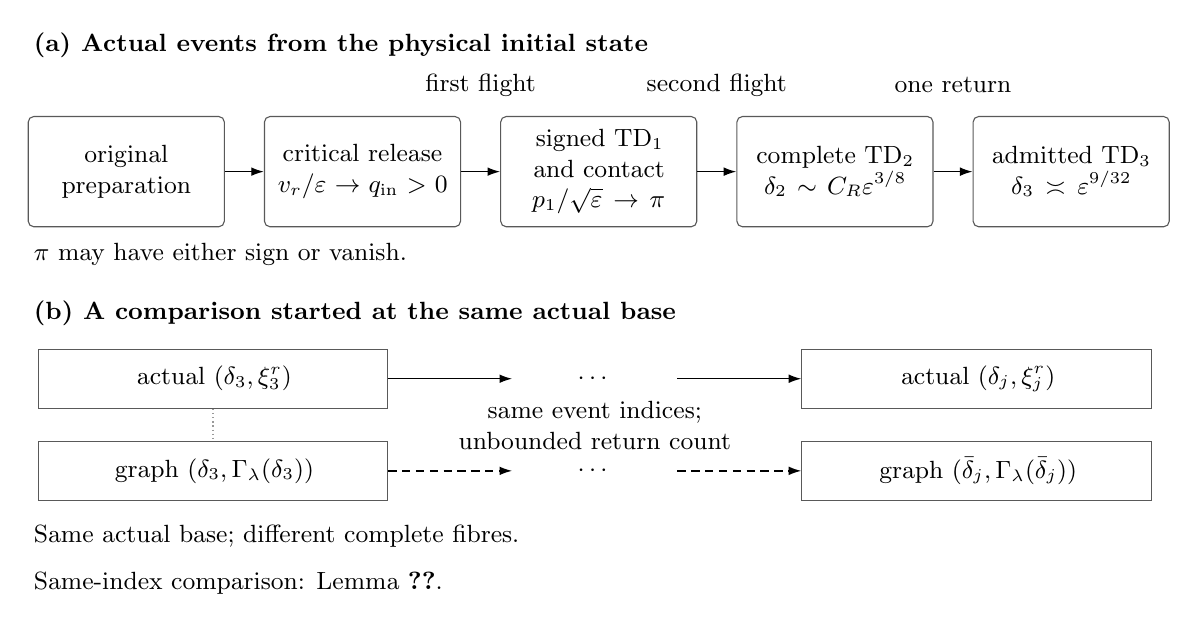
\begin{tikzpicture}[
 x=1cm,y=1cm,font=\small,
 every node/.style={inner sep=2pt},
 stage/.style={draw=black!65,rounded corners=2pt,align=center,
               text width=2.35cm,minimum height=1.40cm},
 arrow/.style={-{Latex[length=1.6mm,width=1.1mm]},line width=.5pt},
 chain/.style={draw=black!65,align=center,text width=4.3cm,
               minimum height=.75cm},
 guide/.style={draw=black!40,densely dotted,line width=.5pt}
]
 \node[anchor=west,font=\small\bfseries] at (0,7.05)
   {(a) Actual events from the physical initial state};
 \node[stage] (initial) at (1.25,5.45)
   {original\\preparation};
 \node[stage] (release) at (4.25,5.45)
   {critical release\\$v_r/\varepsilon\to q_{\rm in}>0$};
 \node[stage] (tdone) at (7.25,5.45)
   {signed $\mathrm{TD}_1$\\and contact\\$p_1/\sqrt\varepsilon\to\pi$};
 \node[stage] (tdtwo) at (10.25,5.45)
   {complete $\mathrm{TD}_2$\\$\delta_2\sim C_R\varepsilon^{3/8}$};
 \node[stage] (tdthree) at (13.25,5.45)
   {admitted $\mathrm{TD}_3$\\$\delta_3\asymp\varepsilon^{9/32}$};
 \draw[arrow] (initial.east) -- (release.west);
 \draw[arrow] (release.east) -- (tdone.west);
 \draw[arrow] (tdone.east) -- (tdtwo.west);
 \draw[arrow] (tdtwo.east) -- (tdthree.west);
 \node at (5.75,6.55) {first flight};
 \node at (8.75,6.55) {second flight};
 \node at (11.75,6.55) {one return};
 \node[anchor=west] at (0,4.40) {$\pi$ may have either sign or vanish.};

 \node[anchor=west,font=\small\bfseries] at (0,3.65)
   {(b) A comparison started at the same actual base};
 \node[chain] (actualstart) at (2.35,2.82)
   {actual $(\delta_3,\xi_3^r)$};
 \node[chain] (graphstart) at (2.35,1.65)
   {graph $(\delta_3,\Gamma_\lambda(\delta_3))$};
 \node[chain] (actualend) at (12.05,2.82)
   {actual $(\delta_j,\xi_j^r)$};
 \node[chain] (graphend) at (12.05,1.65)
   {graph $(\bar\delta_j,\Gamma_\lambda(\bar\delta_j))$};
 \draw[arrow] (actualstart.east) -- (6.15,2.82);
 \node at (7.20,2.82) {$\cdots$};
 \draw[arrow] (8.25,2.82) -- (actualend.west);
 \draw[arrow,densely dashed] (graphstart.east) -- (6.15,1.65);
 \node at (7.20,1.65) {$\cdots$};
 \draw[arrow,densely dashed] (8.25,1.65) -- (graphend.west);
 \draw[guide] (actualstart.south) -- (graphstart.north);
 \node[fill=white,align=center] at (7.20,2.23)
   {same event indices;\\unbounded return count};
 \node[anchor=west] at (0,.82)
   {Same actual base; different complete fibres.};
 \node[anchor=west] at (0,.22)
   {Same-index comparison: Lemma~\ref{sel:sharp-phase}.};
\end{tikzpicture}
\caption{From the physical preparation to the same-base return
comparison. (a) Both preparatory flights and the intervening signed
contact are generated by the original trajectory.
(b) The graph starts at the actual third-touchdown base, with a small
complete fibre discrepancy. The actual normal memory is retained;
the two starting states are not identical.
Arrows and spacing are schematic, not physical time.}
\label{fig:entry-comparison}
\end{figure}


\subsection{Normalized touchdown coordinates and the finite-scale reference}

The return sends an input scale $\delta$ to
$D\asymp\delta^{3/4}$. Under the bounds below, its tangential
correction has size $O(\delta)=O(D^{4/3})$. The normal correction
has size $O(\delta D)=O(D^{7/3})$ after the actual touchdown equation
eliminates the larger release-velocity terms. These cancellations,
proved in Appendix~\ref{sec:detuned-return}, motivate the powers
$4/3$ and $7/3$ in the normalized state.

Use the slips $u_r,u_0=u_r+r$ defined in Section~\ref{sec:model},
and put $r_0=c_\lambda/3$. At a touchdown with $p=-a\delta<0$, the independent coordinates are
\begin{equation}
 \begin{gathered}
 y=z=\eps\delta^2\zeta,\qquad
 u_r=d_\lambda\delta+d_\lambda\delta^{4/3}\eta_U^r,\qquad
 v=-r_0\delta^2-r_0\delta^{7/3}\eta_W,\\
 \xi^r=(\zeta,\eta_U^r,\eta_W),\qquad
 W=1+\delta^{1/3}\eta_W.
 \label{loc:tuple}
 \end{gathered}
\end{equation}
If $p(\phi_\delta)=-a\delta$ on the chosen positive-cosine branch,
the physical inverse is
\begin{equation}
 (\phi,y,\omega,v,z)
 =\left(\phi_\delta,\eps\delta^2\zeta,
       \frac{u_r+r-U_*}{\cos\phi_\delta},v,\eps\delta^2\zeta\right).
 \label{loc:inverse}
\end{equation}
Thus $b$ and $\eta_B=(-b-c_\lambda\delta)/(c_\lambda\delta^{4/3})$
are dependent coordinates. Fix a closed ball $\Kcal$ in the independent
coordinates with $0$ and all $\xi_{*,\lambda}$ in its interior.
Lemma~\ref{lem:td2-complete-preparation} bounds the original second-touchdown
independent tuples uniformly. Choose $M_{\rm in}$ once so that its ball
contains these tuples and $\Kcal$ strictly in its interior.
This choice does not change the fixed slip threshold $M_{\rm sl}$.
Fix $0<\gamma_{\rm cl}<\frac12\min_\lambda r_0$.
The physical input domain is
\begin{equation}
 |\xi^r|\le M_{\rm in},\quad r_0W-\zeta\ge\gamma_{\rm cl}>0,
 \quad 0<\eps\le C_0\delta^2,
 \quad 0\le r\le A\delta^{4/3},\qquad e=\eps\delta^{-3/2}.
 \label{loc:domain}
\end{equation}
The closing margin is $\dot z-v=\delta^2(r_0W-\zeta)$.
There is no positive lower bound on $e$ or $r$.
Taylor expansion in the chart $(p,y,u_0,v)$ gives
\begin{equation}
 \eta_B=\frac{g_b}{c_\lambda}
       \left(\eta_U^r+\frac{r}{d_\lambda\delta^{4/3}}\right)
       +O(\delta^{2/3}),\qquad g_b=-d_\lambda b_u(G),
 \label{loc:dependent}
\end{equation}
where $b_u$ is the derivative with respect to $u_0$.
The identity $-ab_p(G)+d_\lambda b_u(G)=-c_\lambda$ supplies the
leading cancellation; see Lemma~\ref{ret:inverse}.

The limiting return is defined at a fixed positive input scale
$\delta$, with $\eps,r\to0$. Physical displacement and memory then
vanish, but their normalized values still determine the release speed.
The later expansion $\delta\downarrow0$ is used to construct the graph
and its phase. To define this exact return $T_{0,\lambda}=(f_0,h_0)$,
set $r=0$ and use identical values of the independent coordinates $\xi$.
Put $\sigma=\sqrt\delta$ and
$h_\delta=\mu A(\phi_\delta)-B(\phi_\delta)$.
Use the compression clock $\tau_c=\sqrt\delta(t-t_{\rm in})/\eps$
and scalings $(y,z)=\eps\delta^{3/2}(Y,Z)$, $v=\delta^2V_c$
and $u_0=\delta\mathcal U$.
With primes denoting $\tau_c$ derivatives, the saturated compression
reference solves
\begin{equation}
 \begin{gathered}
 Y'=V_c,\quad \sigma Z'=Y-2Z,\quad
 V_c'=-a(Z-Y),\quad \mathcal U'=-h_\delta(Z-Y),\\
 (Y,Z,V_c,\mathcal U)(0)=
 (\sigma\zeta,\sigma\zeta,-r_0W,
            d_\lambda(1+\delta^{1/3}\eta_U)).
 \label{loc:compression}
 \end{gathered}
\end{equation}
At its first arrest $\mathcal U=0$, switch to the elapsed release
clock $\tau_r=(t-t_{\rm arrest})/\eps$ and velocity
$v=\delta^{3/2}V$. Thus $V=\sqrt\delta V_c$ at arrest, while
$Y$ and $Z$ keep their compression scalings. With primes now denoting
$\tau_r$ derivatives, the inherited normal motion $N=(Y,V,Z)$ solves
\begin{equation}
 N'=A_DN,\qquad
 A_D=\begin{pmatrix}0&1&0\\-1/2&0&1/2\\1&0&-2\end{pmatrix},
 \qquad N(0)=(Y,\sigma V_c,Z)_{\rm arrest}.
 \label{loc:normal-reference}
\end{equation}
If $R_0$ is its first force zero and $Q=V(R_0)$, reconstruct the
physical release as
$(p,y,u_0,v,z)=(-a\delta,0,0,\delta^{3/2}Q,0)$.
Its exact free mechanical flow to the first subsequent touchdown
defines $T_{0,\lambda}$. This retains the finite $\sqrt\delta$
compression and its inherited memory; the zero physical memory is
introduced only in the release reconstruction.

For the initial state $(-2,0,-1)$,
Lemma~\ref{con:normal-opening} gives $Y=Z=-\gamma_\#$ and
$V=\nu_\#$ at the first release, with
$\nu_\#>\gamma_\#>0$. Define
\begin{equation}
 \begin{gathered}
 q_\lambda=\nu_\#\sqrt{r_0d_\lambda/h+ad_\lambda^2/(2h^2)},
 \qquad K_\lambda=\sqrt{6q_\lambda/c_\lambda},\\
 \varkappa_W=\tfrac12+\frac{3g_b}{2c_\lambda},\qquad
 \xi_{*,\lambda}=K_\lambda^{-4/3}(0,-1,-\varkappa_W).
 \label{loc:constants}
 \end{gathered}
\end{equation}

\subsection{Preparation of the original trajectory}

Preparation serves two purposes. Its third-touchdown state must be
accurate enough for repeated return comparison and for the entrance
phase in Section~\ref{sec:graph}. The whole preceding trajectory
must also approach the prescribed incoming arc, so that later returns
can be attached to it. We first record the state estimates and then
the bounds on the intervening motion.

The capture and critical-passage estimates give a first release with
$v_r=\eps(q_{\rm in}+o(1))$, negative normal memory and a strict
opening margin. Here $q_{\rm in}>0$ depends only on $(\lambda,\theta)$,
while $p_r/\sqrt\eps\to H=ak/\gamma$ and
$b_r/\sqrt\eps\to-\ell H$
(Theorem~\ref{thm:detuned-release}). With $c=c_\lambda$, the
preparation constants are
\begin{equation}
 \begin{gathered}
 cT_f^2+3\ell HT_f=6q_{\rm in},\quad T_f>0,
 \qquad \pi=H-aT_f,\\
 S=d_\lambda T_f,\quad Q=T_f(\ell H/2+cT_f/3),\quad
 A_{\rm reb}^2=QS/h-\pi S^2/(2h^2),\\
 R=\nu_\#A_{\rm reb},\qquad C_R=\sqrt{6R/c}.
 \label{loc:preparation-constants}
 \end{gathered}
\end{equation}
The scale $r=k\sqrt\eps$ balances this first flight: with
$t=\sqrt\eps\,T$, the terms $v_rt$, $b_rt^2/2$ and $-ct^3/6$
in \eqref{prep:gap-expansion} all have order $\eps^{3/2}$.
The smaller memory value still determines opening on $t=O(\eps)$
through $q_{\rm in}+Y_r^0>0$. Thus the same original preparation
supplies the positive release coefficient and inherited memory for
both exceptional flights.
At the first touchdown, $p_1=p(t_1)$ satisfies
$p_1/\sqrt\eps\to\pi$. Here $\sqrt\eps$ is the preparation scale,
and $\pi$ may be positive, zero or negative. Its arrest margin is
\[
 2hQ-\pi S
 =T_f\{\gamma H+(2hc/3+ad_\lambda)T_f\}>0.
\]
The signed contact theorem applies with $r=k\sqrt\eps$ and yields
$v_L=\eps^{3/4}(R+o(1))$ and
$y_L=z_L=-\eps^{7/4}(\gamma_\#A_{\rm reb}+o(1))$.
In particular both $R$ and $R-\gamma_\#A_{\rm reb}$ have common
positive lower bounds.

The ensuing touchdown occurs after an elapsed time $T$ and has scale
$D=-p(T)/a=C_R\eps^{3/8}(1+o(1))$. To obtain its complete tuple,
one must eliminate the release velocity before dividing by the finer
normal scale. A separate release-velocity approximation would be
amplified by that division. At the actual root $y(T)=z(T)$, direct integration gives
\begin{equation}
 -v(T)-\frac c3D^2
 =\frac{y_L-z(T)}T-\frac12b_LT+\frac c3(T^2-D^2)
 -\frac1{2T}\int_0^T(T^2-t^2)(\dot b(t)+c)\,\dd t.
 \label{loc:touchdown-cancellation}
\end{equation}
The tangential and acceleration numerators are $O(\sqrt\eps)$,
and this normal numerator is $O(\eps^{7/8})$.
Their denominators $D^{4/3},D^{4/3},D^{7/3}$ have exactly these
orders. Thus the actual second touchdown has a bounded full tuple,
negative memory, a strict closing margin, and
$r/D^{4/3}=kC_R^{-4/3}(1+o(1))$; see
Lemma~\ref{lem:td2-complete-preparation}.

\begin{proposition}[The original prepared entrance]
\label{loc:entrance}
Under the standing model convention, all the following estimates are
uniform on the prescribed compact label classes.
The original trajectory has an admitted third touchdown with
\begin{equation}
 \begin{gathered}
 \delta_2=C_R\eps^{3/8}(1+o(1)),\qquad
 \delta_3\asymp\eps^{9/32},\quad
 r/\delta_3^{4/3}=O(\eps^{1/8}),\\
 \left|\log\frac{\delta_3}{K_\lambda\delta_2^{3/4}}\right|
 +|\xi_3^r-\xi_{*,\lambda}|+
 |\eta_{B,3}-(g_b/c)\eta_{U,*,\lambda}|
 \le C\eps^{3/32}.
 \label{loc:third-entry}
 \end{gathered}
\end{equation}
Here $\eta_{U,*,\lambda}$ is the slip component of $\xi_{*,\lambda}$.
The third touchdown retains the full cone, inverse branch, negative
normal memory, strict closing margin and all inequalities of
\eqref{loc:domain}, so it is a new admitted input. The preparation scale
$\sqrt\eps$ is followed by touchdown scales $\eps^{3/8}$ and
$\eps^{9/32}$; only at the last does the normalized state approach
$\xi_{*,\lambda}$.
All estimates are uniform on the fixed compact label classes and
are obtained from the original physical initial state.


The entrance constant
\begin{equation}
 \chi_\lambda(\mathfrak a)=\chi_{\lambda,\theta}(k)
   =3\log K_\lambda-\tfrac34\log C_R(\lambda,k,\theta),
 \qquad \mathfrak a=(k,\theta,\nu,\mathbf n),
 \label{sel:chi}
\end{equation}
is continuous, bounded and independent of $\nu,\mathbf n$. Moreover,
\begin{equation}
 \log(K_\lambda^4/\delta_3^{\mathfrak a})
 =\tfrac9{32}\log(1/\eps)+\chi_\lambda(\mathfrak a)
                      +r_{\mathfrak a}^{\log}(\eps),
 \qquad \sup_{\mathfrak a}|r_{\mathfrak a}^{\log}(\eps)|\to0.
 \label{loc:log-entry}
\end{equation}
On each fixed closed incoming rigid subarc the original motion
approaches that prescribed arc. For each fixed small $\eta>0$,
its remaining prefix from $p=\eta$ through $\TD_3$ is contained in
$G+B_{C\eta+o(1)}$ in the full physical state. The motion has positive
$p$ up to the descending-slip threshold, and its mechanical distance
from $G$ tends uniformly to zero from that threshold through $\TD_3$.
\end{proposition}
\begin{proof}
Lemma~\ref{lem:td2-complete-preparation} and
Corollary~\ref{cor:original-to-td2} give the complete second input
and its uniform scale asymptotic. Applying Theorems~\ref{thm:detuned-value-bridge}
and~\ref{thm:detuned-output-admission} to this input, as in
Corollary~\ref{cor:td3-admission}, gives \eqref{loc:third-entry}
and the stated admissibility of the returned state.
The normalized first-release data are continuous and have common
positive margins by Lemma~\ref{lem:critical-pullback} and
Theorem~\ref{thm:detuned-release}. The formulas
\eqref{loc:preparation-constants} therefore give common positive
bounds and continuity for $C_R$. Set
\[
 e_{\mathfrak a}(\eps)
 =\log\frac{\delta_2^{\mathfrak a}}
                 {C_R(\mathfrak a)\eps^{3/8}}.
\]
The second-touchdown root estimates are uniform, so
$\sup_{\mathfrak a}|e_{\mathfrak a}|\to0$.
Taking logarithms in \eqref{loc:third-entry} gives
$r_{\mathfrak a}^{\log}=-\tfrac34 e_{\mathfrak a}
+O(\eps^{3/32})$, proving \eqref{loc:log-entry}.
The second-touchdown remainder needs no specified rate.

On a closed incoming arc $p\ge\eta$, the unilateral capture estimate
in the proof of Lemma~\ref{lem:detuned-threshold} bounds the full scaled normal
state through any initial departures and recontacts. Capture takes
a common finite fast time, produces an $O(\eps)$ slow increment,
and is followed by an $O(\eps)$ integrated slow-field discrepancy
from the prescribed saturated rigid orbit; see
\eqref{ent:fixed-initialization}. Gronwall's inequality gives convergence
to that particular rigid subarc. Throughout it
$|y|+|z|=O_\eta(\eps^2)$ and $|v|=O_\eta(\eps)$, so the fast
excursion collapses to its original physical starting point.

For the remaining incoming segment, the entry estimates
\eqref{ent:safe-tracking} control the normal state and its effect
on the slow variables up to the descending-slip threshold.
They apply on every stopped interval before that threshold, including
the final $p\asymp\sqrt\eps$ annulus. The weak-coordinate bounds
and analytic chart put this segment in $G+B_{C\eta+o(1)}$; it remains
at positive $p$ until that threshold. The stopped comparison in
Theorem~\ref{thm:detuned-release} controls every prefix through its first
force zero, with mechanical distance
$O(\sqrt\eps+\eps(1+|\log\eps|))$ from $G$.
Proposition~\ref{prep:first-flight} gives duration and mechanical state
distance $O(\sqrt\eps)$ through the first exceptional touchdown.
The ensuing contact uses the first application of
Theorem~\ref{con:contact-release}, with scale $\sqrt\eps$ and
$r=O(\sqrt\eps)$; its complete prefix bound is $O(\sqrt\eps)$.
The second exceptional flight has duration and mechanical state
distance from $G$ both $O(\eps^{3/8})$. The full-prefix estimates
leading to Corollary~\ref{cor:original-to-td2} control these passages
and supply the actual complete $\TD_2$ cone.
Apply the contact prefix estimate \eqref{con:prefix} and
Lemma~\ref{lem:paired-free-normalization} to the
$\TD_2\to\TD_3$ return at $\delta_2\asymp\eps^{3/8}$.
Its mechanical distance from $G$ is $O(\eps^{9/32})$ and its memory
tends to zero. These bounds include both exceptional flights, their
contacts and the passage to $\TD_3$, and prove the stated original-prefix
localization.

\end{proof}

\subsection{The return estimate and its domains}

Let $\|\cdot\|_{1,*}$ include values and first derivatives with
respect to $\delta\partial_\delta$ and $\xi$.
The following conclusions collect
Proposition~\ref{prop:limiting-factorization} and
Theorems~\ref{thm:detuned-value-bridge}--\ref{thm:detuned-output-admission}.
Write the actual return as
\[
 T_{\eps,r}(\delta,\xi^r)=(D,\xi^{r,+})
   =\bigl(f_{\eps,r}(\delta,\xi^r),h_{\eps,r}^r(\delta,\xi^r)\bigr).
\]
The reference derivatives construct the invariant graph; the value
error controls the actual iterates; the output conditions allow the
next return. All constants are uniform on the fixed compact model
classes and the prescribed finite input bounds.

\begin{proposition}[The complete local return]
\label{loc:return}
For sufficiently small $\delta$, the following statements hold.
\begin{enumerate}[label=\textup{(\roman*)}]
\item \emph{Reference regularity.} On a bounded convex auxiliary fibre
domain $\Omega$ containing the fixed independent input ball and $\Kcal$,
the exact reference has a $C^1$ extension with
\begin{equation}
 \begin{aligned}
 \left\|\log\frac{f_0}{K_\lambda\delta^{3/4}}\right\|_{1,*}
       +\|h_0-\xi_{*,\lambda}\|_{1,*}&\le C\delta^{1/4},\\
 |D_\xi\log f_0|+|D_\xi h_0|&\le C\delta^{1/3}.
 \end{aligned}
 \label{loc:factorization}
\end{equation}
The reference map and its state derivatives are jointly continuous in
$\lambda$. The memory component of $h_0$ vanishes.
\item \emph{Compliant value approximation.} On the physical domain
\eqref{loc:domain},
the actual first contact--flight return exists, retains its negative
memory and transverse first-event margins, and satisfies
\begin{equation}
 \left|\log\frac{f_{\eps,r}(\delta,\xi^r)}{f_0(\delta,\xi^r)}\right|
 +|h_{\eps,r}^r(\delta,\xi^r)-h_0(\delta,\xi^r)|
 \le C(e+r/\delta).
 \label{loc:value}
\end{equation}
\item \emph{Admissibility of the returned state.} There are common radii
$0<\delta_{\rm reset}<\delta_{\rm g}<\delta_{\rm call}$ such that
a physical input satisfying \eqref{loc:domain} with
$\delta\le\delta_{\rm reset}$ has output $D$ satisfying
\begin{equation}
 \begin{gathered}
 \delta<D<\delta_{\rm g},\quad \xi^{r,+}\in\operatorname{int}\Kcal,
 \quad \eps<C_0D^2,\quad r\le AD^{4/3},\\
 \left|\log\frac D{K_\lambda\delta^{3/4}}\right|
       +|\xi^{r,+}-\xi_{*,\lambda}|
       \le C(\delta^{1/4}+e+r/\delta).
 \label{loc:admission}
 \end{gathered}
\end{equation}
It has $u_r^+>0$, $v^+<0$, $y^+=z^+<0$, the same inverse branch,
a bounded dependent coordinate and the strict closing margin.
Another return requires $D\le\delta_{\rm reset}$.
The outer radius may be reduced first, with the reset radius chosen
afterwards.
\end{enumerate}
\end{proposition}

The auxiliary extension in \eqref{loc:factorization} continues the
signed linear reference even when initial force is negative.
For physical inputs, the proof of \eqref{loc:value} first compares the
actual return with a reference $R^r$ reconstructed at slip
$u_{0,L}=r$. This costs $Ce$. The references $R^r$ and $T_0$ share
the entire finite-scale compression and inherited release, and their
free flights differ by $Cr/\delta$. Finally the actual output is
recoded by
\[
 h_{\eps,r}^r=h_{\eps,r}^0-
                  \frac{r}{d_\lambda D^{4/3}}(0,1,0).
\]
The paired free-flight estimate has already established
$D^{4/3}\asymp\delta$, so this last cost is also $Cr/\delta$.
The contact comparison retains both tail moments and the inherited
normal state. In the elapsed release time $\rho$ of
Appendix~\ref{sec:contact}, put $w=u_r/\eps$, $L=Z-Y$ and
$\vartheta=B/A$. The normal-velocity projection is
\[
 \begin{gathered}
 P=\widehat V-e\vartheta w,\qquad \widetilde N=(Y,P,Z),\\
 \widetilde N'=A_D\widetilde N+eF,\qquad
 F=(\vartheta w,b-\vartheta a_T-\vartheta'w,0).
 \end{gathered}
\]
where primes denote $\rho$ derivatives and
$\vartheta'=\eps\vartheta_\phi\dot\phi$.
The exact identity $C-B^2/A=1/2$ cancels the term containing $w'$
when the normal and slip equations are combined. Thus $F$ is bounded
on the stopped boxes without estimating the stiff slip derivative.
The full stopped-prefix estimates and first-release brackets are
proved in \eqref{con:projection}--\eqref{con:release-mechanics}.
Only the exact reference return is differentiated in
\eqref{loc:factorization}; \eqref{loc:value} compares values of the
actual compliant map.


\section{The exact graph and comparison of actual returns}
\label{sec:graph}
The logarithmic form of the exact limiting return contracts the
complete independent state. We use it to construct an invariant graph
and a normalized scalar coordinate that records progress along its
returns. This coordinate fixes the explicit compliance sequences in
Theorem~\ref{thm:common-free}. The corresponding finite-scale contact and
free curves retain the order of motion needed for path comparison.

\begin{proposition}[An exact graph and normalized phase]
\label{prop:canonical-graph-phase}
After decreasing the outer radius $\delta_{\rm g}$, there are a common
radius $0<\delta_0<\delta_{\rm g}$ and a jointly
continuous graph $\Gamma_\lambda:(0,\delta_{\rm g}]\to\Kcal$,
with zero memory component, such that
\begin{equation}
 \begin{aligned}
 |\Gamma_\lambda(d)-\xi_{*,\lambda}|&\le Cd^{1/3},\\
 |\Gamma_\lambda(d_2)-\Gamma_\lambda(d_1)|
 &\le C\max(d_1,d_2)^{1/3}|\log(d_2/d_1)|.
 \end{aligned}\label{gr:graph-bounds}
\end{equation}
Its base map $F_\lambda(d)=f_{0,\lambda}(d,\Gamma_\lambda(d))$
is strictly increasing, $F_\lambda(d)>d$, and
$\sup_\lambda F_\lambda(\delta_0)<\delta_{\rm g}$. For
$0<d\le\delta_0$,
\begin{equation}
 T_{0,\lambda}(d,\Gamma_\lambda(d))
      =(F_\lambda(d),\Gamma_\lambda(F_\lambda(d))).
 \label{gr:invariance}
\end{equation}
On the outer interval there is a jointly continuous phase
$\mathcal S_\lambda$, strictly decreasing and bi-Lipschitz in $\log d$,
such that, with $\rho_c=3/4$,
\begin{equation}
 \mathcal S_\lambda(F_\lambda(d))
       =\rho_c\mathcal S_\lambda(d),\qquad
 \mathcal S_\lambda(d)=\log(K_\lambda^4/d)+O(d^{1/3}).
 \label{eq:canonical-Schroeder}
\end{equation}
The equation holds on the inner interval. The normalization fixes its
germ at zero on this graph. All bounds are uniform in $\lambda$.
\end{proposition}
\begin{proof}
Put $x=\log(K_\lambda^4/\delta)$ and
$\eta=\xi-\xi_{*,\lambda}$. Proposition~\ref{prop:limiting-factorization} gives
\begin{equation}
 \widehat T_\lambda(x,\eta)
  =(\rho_c x+r_\lambda(x,\eta),H_\lambda(x,\eta)),\qquad
 |r|+|H|+|Dr|+|DH|\le Ce^{-x/4}.
 \label{gr:log-map}
\end{equation}
For each $\lambda$ the domain
$[X,\infty)\times(\Omega-\xi_{*,\lambda})$ is convex. In the norm
$\|(x,\eta)\|=\max\{|x|,\|\eta\|_\infty\}$ its derivative row
sums are at most $\rho_c+Ce^{-X/4}$. Increase $X$ to obtain
\begin{equation}
 \|\widehat T_\lambda(z)-\widehat T_\lambda(\widetilde z)\|
       \le q\|z-\widetilde z\|,\qquad q=7/8.
 \label{gr:contraction}
\end{equation}
The base segment here is logarithmic, hence geometric interpolation
of its endpoint scales. It lies in the auxiliary domain of the exact
reference; actual returns will be compared by
\eqref{loc:value} at their physical endpoints.

We seek a curve $V_\lambda(S)=(S+u_\lambda(S),v_\lambda(S))$,
$S\ge S_0$, whose parameter is multiplied by $\rho_c$ under the return:
\[
 V_\lambda(\rho_c S)=\widehat T_\lambda(V_\lambda(S))
 \qquad(S\ge S_0/\rho_c).
\]
Thus $S$ will be the phase coordinate. To solve for the value at $S$,
evaluate the right-hand side at $S/\rho_c$. The error
$e^{-x/4}$ in \eqref{gr:log-map} then has size
$e^{-S/(4\rho_c)}=e^{-S/3}$, which determines the weight below.
On continuous pairs for $S\ge S_0$ set
$\|Z\|_0=\sup_{S\ge S_0}e^{S/3}(|u(S)|+\|v(S)\|_\infty)$,
and, writing $t=S/\rho_c$, define
\[
 (\mathcal PZ)(S)=
 \bigl(\rho_c u(t)+r_\lambda(t+u(t),v(t)),
                 H_\lambda(t+u(t),v(t))\bigr).
\]
On any fixed norm ball, all arguments lie in the common auxiliary
domain for large $S_0$. Since
$e^{S/3-t/4}=1$ and $e^{S/3-t/3}=e^{-S/9}$,
\[
 \|\mathcal P0\|_0\le C,\qquad
 \|\mathcal PZ-\mathcal P\widetilde Z\|_0
 \le(\rho_c e^{-S_0/9}+C_Me^{-4S_0/9})
                       \|Z-\widetilde Z\|_0.
\]
Choose $M\ge\max(1,2C)$ and then $S_0$ so the last coefficient
is below $1/2$. The fixed point satisfies
\begin{equation}
 u,v=O(e^{-S/3}),\qquad
 V_\lambda(S)=\widehat T_\lambda(V_\lambda(S/\rho_c)).
 \label{gr:parametrized-graph}
\end{equation}

The Picard iterates from zero are $C^1$. Their weighted derivative
norms $A_n=\sup e^{S/3}(|u_n'|+\|v_n'\|_\infty)$ obey
\[
 A_{n+1}\le C+(e^{-S_0/9}+C_Me^{-4S_0/9})A_n
\]
by the chain rule and \eqref{gr:log-map}. They are uniformly bounded.
Passing to the uniform limit in the integral inequality gives
\begin{equation}
 |u(b)-u(a)|+\|v(b)-v(a)\|_\infty
       \le C\int_a^b e^{-t/3}\dd t\quad(S_0\le a<b).
 \label{gr:weighted-Lipschitz}
\end{equation}
Finite iterates are jointly continuous in $(\lambda,S)$ on compact
intervals, and their common contraction tail preserves this continuity.
This argument uses only first state derivatives of the limiting return.

For larger $S_0$, choose $\eta<1/2$ with $Ce^{-S_0/3}\le\eta$.
Writing $x=S+u_\lambda(S)$, \eqref{gr:weighted-Lipschitz} gives
\begin{equation}
 (1-\eta)|S_2-S_1|\le|x_2-x_1|
                  \le(1+\eta)|S_2-S_1|.
 \label{gr:phase-bilip}
\end{equation}
Thus $S\mapsto x$ is strictly increasing and bi-Lipschitz.
On each fixed positive base interval this also gives two-sided
Lipschitz control between the phase and the base itself. Define
\begin{equation}
 \delta_\lambda(S)=K_\lambda^4e^{-S-u_\lambda(S)},\quad
 \Gamma_\lambda(\delta_\lambda(S))=\xi_{*,\lambda}+v_\lambda(S),\quad
 \mathcal S_\lambda(\delta_\lambda(S))=S.
 \label{gr:phase-definition}
\end{equation}
Choose $\delta_{\rm g}<\min_\lambda \delta_\lambda(S_0)$ and
$\delta_0<\min_\lambda \delta_\lambda(S_0/\rho_c)$, within the
limiting-return radii. Reduce $\delta_0$ so that
$\sup_\lambda F_\lambda(\delta_0)<\delta_{\rm g}$.
Equation \eqref{gr:parametrized-graph} gives
$F_\lambda(\delta_\lambda(S))=\delta_\lambda(\rho_c S)>\delta_\lambda(S)$
on the inner interval. Both factors are strictly decreasing in their
arguments, so $F_\lambda$ is strictly increasing there. It remains
strictly increasing on the outer interval after reducing its radius:
\eqref{loc:factorization} and \eqref{gr:weighted-Lipschitz} give a
positive lower bound for its logarithmic difference quotient.
The same estimates give \eqref{gr:graph-bounds} and \eqref{eq:canonical-Schroeder}.
The memory component of the fibre map vanishes, hence so does
that of the graph.
For two coordinates with the stated normalization on this graph,
their difference satisfies
$E(d)=\rho_c^jE(F_\lambda^{-j}(d))\to0$, proving uniqueness
of the normalized germ. The unconstrained part of the outer interval
is only a representative of that germ.
\end{proof}

The graph's logarithmic Lipschitz constant on $(0,\delta_{\rm g}]$
is $L_\Gamma\le C\delta_{\rm g}^{1/3}$. Reduce this outer radius,
and then $\delta_0$, so that $q(1+L_\Gamma)<1$. With the common
graph domains fixed, choose $\delta_{\rm reset}$ last as in
Theorem~\ref{thm:detuned-output-admission}, and take $s_0>0$ with
$2s_0<\min(\delta_0,\delta_{\rm reset})$. All reference curves with
input in a fixed positive compact subset of $(0,2s]$ are then
available in the same construction.

\subsection{The ordered one-return curve}
\label{gr:ordered-reference}

We spell out the finite-scale curve used in the path comparison.
Let $p(\phi_d)=-ad$ on the selected branch and put
$h_d=\mu A(\phi_d)-B(\phi_d)>0$. Write
$\Gamma_\lambda(d)=(0,\Gamma_U(d),\Gamma_W(d))$ and define
\begin{equation}
 \begin{gathered}
 U_d=d_\lambda d\{1+d^{1/3}\Gamma_U(d)\},\qquad
 V_d^{\rm in}=-r_0d^2\{1+d^{1/3}\Gamma_W(d)\},\\
 V_d^{\rm a}=V_d^{\rm in}-(ad/h_d)U_d,\qquad
 \mathcal E_\lambda(d,u,v)
     =(\phi_d,0,(u-U_*)/\cos\phi_d,v,0).
 \end{gathered}\label{gr:embedding}
\end{equation}
Here $u$ denotes the tuned slip argument of the embedding. Run the exact
reference compression at $\sigma=\sqrt d$:
\begin{equation}
 Y'=V_c,\quad \sigma Z'=Y-2Z,\quad
 V_c'=-a(Z-Y),\quad \mathcal U'=-h_d(Z-Y),
 \label{gr:compression}
\end{equation}
from $(Y,Z,V_c,\mathcal U)=(0,0,V_d^{\rm in}/d^2,U_d/d)$.
At its first arrest, start the inherited reference
$N_d'=A_DN_d$, $N_d=(Y_d,V_d^{\rm n},Z_d)$, with
$N_d(0)=(Y,\sigma V_c,Z)$ at arrest. Let $R_d$ be its first
force zero. The first-event margins from Section~\ref{sec:contact} give
\begin{equation}
 Z_d(R_d)=Y_d(R_d)<0,\quad V_d^{\rm n}(R_d)>0,\quad
 V_d^{\rm n}(R_d)+Z_d(R_d)>0.
 \label{gr:release-signs}
\end{equation}
Put $V_d^{\rm rel}=d^{3/2}V_d^{\rm n}(R_d)$ and
$\mathcal R_d=\mathcal E_\lambda(d,0,V_d^{\rm rel})$.
Write $\Phi_{\rm f}(\ell;\mathcal R_d)$ for the analytic free
mechanical flow, with zero memory appended. Its first subsequent
touchdown has elapsed time $T_d$ and scale $F_\lambda(d)$.

The continuous ordered curve is
\begin{equation}
 \cC_{\lambda,d}(\alpha)=
 \begin{cases}
 \mathcal E_\lambda(d,(1-\alpha)U_d,
                  V_d^{\rm in}-(ad/h_d)\alpha U_d),&0\le\alpha\le1,\\
 \mathcal E_\lambda(d,0,d^{3/2}V_d^{\rm n}((\alpha-1)R_d)),&1\le\alpha\le2,\\
 \Phi_{\rm f}((\alpha-2)T_d;\mathcal R_d),&2\le\alpha\le3.
 \end{cases}\label{eq:ps2-reference-path}
\end{equation}
The compression invariant
$V_c-(a/h_d)\mathcal U=V_d^{\rm in}/d^2-(a/h_d)U_d/d$
gives $d^{3/2}V_d^{\rm n}(0)=V_d^{\rm a}$, so the first join agrees.
The second join is $\mathcal R_d$. For $0<d\le\delta_0$, graph invariance gives
\begin{equation}
 \cC_{\lambda,d}(3)=\cC_{\lambda,F_\lambda(d)}(0),\qquad
 \sup_\alpha|\cC_{\lambda,d}(\alpha)-G|\le Cd^{3/4}.
 \label{gr:curve-joins}
\end{equation}
The contact pieces have instantaneous physical duration in this
reference curve; their parameters preserve the order of compression
and release. They are not extra free solutions. At every fixed
positive compact input interval, including the enlarged intervals
used to scan $[s/2,2s]$, the event maps, free flow and graph bound
make \eqref{eq:ps2-reference-path} Lipschitz in its input, uniformly in $\lambda$.
The corresponding constants may depend on that interval.

The same radius choice makes $U_d>0$. Consequently the contact
curve is injective on $[0,2]$: the tuned slip $(1-\alpha)U_d$
strictly decreases on compression, while on release it is zero
and the normal velocity satisfies
\begin{equation}
 \frac{\dd V_d^{\rm n}}{\dd\tau}
       =\tfrac12(Z_d-Y_d)>0\qquad(0\le\tau<R_d).
 \label{gr:contact-injectivity}
\end{equation}
Positivity of the active force gives the strict inequality, and
the two pieces meet only at their common arrest point. We will use
this fact both to identify an interior stopping target and to
separate complete path images.

\subsection{The free-section parameter}
\label{gr:free-section}

Along the free part, $\dot p=-a+O(d+\ell)<-a/2$ after the common
radius is reduced. Thus $p$ strictly decreases from $-ad$ to
$-aF_\lambda(d)$. Fix $0<s\le s_0$ and put
$d_*=F_\lambda^{-1}(s)$; this inverse is defined since $F$ is
continuous and strictly increasing from zero and $F(s)>s$.
For $d_*\le d\le s$, the equation
\begin{equation}
 p(\Phi_{\rm f}(\ell_s(d);\mathcal R_d))=-as
 \label{gr:section-root}
\end{equation}
has exactly one root in $[0,T_d]$. Its derivative in $\ell$ is
bounded away from zero, so its continuous dependence, including
the endpoints, follows either from the inverse function theorem
or directly from strict monotonicity and compactness. Hence
\begin{equation}
 j_s(d)=2+\ell_s(d)/T_d,
 \qquad j_s(d_*)=3,\qquad j_s(s)=2
 \label{gr:free-section-definition}
\end{equation}
is the continuous parameter in \eqref{eq:path-free-section}.
On contact the section value is instead the constant $p=-ad$;
therefore its section points have $d=s$ and $0\le\alpha\le2$.
Together these observations give exactly the terminal domain
$\mathcal A_s$ of \eqref{eq:ps5-domain}.

\subsection{Growth, the error budget and the first section}

Fix all compact classes and the finite cones in
Theorem~\ref{thm:detuned-output-admission}.  Reduce the graph outer radius first, and
then take its compatible reset cutoff, so that
\[
 0<\delta_{\rm reset}<\delta_{\rm g}<\delta_{\rm call},\qquad
 q_{\rm g}:=(1+L_\Gamma)q<1,
\]
where $q<1$ is the full logarithmic contraction in
\eqref{gr:contraction} and $L_\Gamma$ is the logarithmic Lipschitz
constant of the graph on the outer interval.  Choose a fixed
$\Delta<\delta_{\rm reset}$ below every inner input cutoff.  It is
also chosen so small that
\begin{equation}
 c_D\Delta^{-1/4}>2,
 \qquad c_D\delta^{3/4}\le\delta^+\le C_D\delta^{3/4}
 \quad(0<\delta\le\Delta),
 \label{path:growth-bounds}
\end{equation}
and the full-prefix tubes below lie in a common neighborhood
$\mathcal U_G$ with $p_\phi\omega<-a/2$.  These choices precede the
choice of the observation section.

Write $\mathcal B_\lambda(d)$ for the value of the dependent
coordinate $\eta_B=(-b-c_\lambda d)/(c_\lambda d^{4/3})$
at the graph state $(d,\Gamma_\lambda(d))$. It is obtained by
substituting that state into the physical inverse \eqref{loc:inverse}
with $\eps=r=0$ and evaluating $b$. In the notation of
Appendix~\ref{sec:detuned-return}, this is
$\mathcal B_{0,0}(d,\Gamma_\lambda(d))$; the corresponding
Lipschitz estimate is \eqref{ret:dependent-Lipschitz}.

\begin{lemma}[Stopped cascade and its complete state budget]
\label{path:stopped-cascade}
For each fixed $0<h\le\Delta$, the actual returns from $\TD_3$ can
be generated, on the original trajectory, up to
\[
 N_h=\min\{n\ge3:\delta_n\ge h\}.
\]
This index is finite, tends to infinity as $\eps\downarrow0$, and
every input used before it is below the reset and inner cutoffs.
The terminal output remains in the graph outer domain.  The complete
cone, inverse branch, negative memory and strict first-event margins
are retained.  Put
\[
 e_n=\eps\delta_n^{-3/2},\quad
 \omega_n=e_n+r/\delta_n,\quad
 B_n=\|\xi_n^r-\Gamma_\lambda(\delta_n)\|_\infty.
\]
For $3\le m\le N_h$,
\begin{align}
 B_m&\le q_{\rm g}^{m-3}B_3+
       C\sum_{n=3}^{m-1}q_{\rm g}^{m-1-n}\omega_n,
       \label{path:graph-budget}\\
 \left|\log\frac{\delta_{n+1}}{F_\lambda(\delta_n)}\right|
       &\le qB_n+C\omega_n\quad(3\le n<N_h),
       \label{path:same-base-output}\\
 \Omega_\eps:=\sup_{3\le n<N_h}\omega_n
       &\le C(\eps^{37/64}+\eps^{7/32})\longrightarrow0.
       \label{path:uniform-defect}
\end{align}
If an actual and a limiting chain are compared in full logarithmic
state, their distance satisfies, through the first output at which
either input chain leaves the common inner domain,
\begin{equation}
 E_m\le q^{m-3}E_3+
          C\sum_{n=3}^{m-1}q^{m-1-n}\omega_n.
 \label{path:two-chain-budget}
\end{equation}
At any sequence of positive-scale inputs whose indices tend to
infinity, the dependent acceleration coordinate also tends to its
graph value.  Thus this convergence concerns the complete normalized
touchdown state, including memory.
\end{lemma}

\begin{proof}
Proposition~\ref{loc:entrance} gives the actual entrance
\begin{equation}
 \delta_3\asymp\eps^{9/32},\qquad
 \eps\le C_0\delta_3^2,\qquad
 r\le A\delta_3^{4/3},\qquad
 x_3=\tfrac9{32}\log(1/\eps)+O(1),
 \quad x=\log(K_\lambda^4/\delta).
 \label{path:entrance}
\end{equation}
The admissibility of the returned state in
Theorem~\ref{thm:detuned-output-admission} and
\eqref{path:growth-bounds} give strict scale growth.  Since $\eps$ and $r=k\sqrt\eps$ stay
fixed on each trajectory, both admissibility inequalities propagate
to the next input.  The return estimate is applied again when its new input
is below $h\le\Delta$.  All events are the
actual first release and subsequent first touchdown, with positive
gap between them.  If there were infinitely many inputs below $h$,
\eqref{path:growth-bounds} would give $\delta_n\ge2^{n-3}\delta_3$,
a contradiction.  Conversely every fixed finite index has
$\delta_n\to0$, by \eqref{path:entrance} and the growth upper bound.
Consequently $N_h\to\infty$ uniformly on the compact classes.

The direct value comparison in
Theorem~\ref{thm:detuned-value-bridge} is made at identical values of the
independent normalized touchdown coordinates and gives a logarithmic output defect at most
$C\omega_n$.  Integrating the derivative bound for the limiting
map along the logarithmic joining segment gives
$E_{n+1}\le qE_n+C\omega_n$, and hence
\eqref{path:two-chain-budget}.  Only the limiting map is
differentiated.  To compare with the graph, take its input at the
actual base $\delta_n$.  Graph invariance and the same argument give
\[
 \max\left\{
 \left|\log\frac{\delta_{n+1}}{F_\lambda(\delta_n)}\right|,
 \|\xi_{n+1}^r-\Gamma_\lambda(F_\lambda(\delta_n))\|_\infty
 \right\}\le qB_n+C\omega_n.
\]
Both output bases are in the outer graph interval.  Correcting the
graph base there costs $L_\Gamma(qB_n+C\omega_n)$, so
$B_{n+1}\le q_{\rm g} B_n+C\omega_n$.  Iteration proves
\eqref{path:graph-budget}.  The bounded entrance error and the two
geometric sums give bounds independent of the number of returns.
Scale growth also gives
\[
 \Omega_\eps\le\eps\delta_3^{-3/2}+r/\delta_3
           \le C(\eps^{37/64}+\eps^{7/32}),
\]
which proves \eqref{path:uniform-defect}.

To compare complete states, recover the acceleration row from the
same physical inverse.
At a common base $d$, the actual and graph arguments differ by
\begin{equation}
 \begin{split}
 \Delta p&=0,\qquad
 \Delta u_0=d_\lambda d^{4/3}
       (\eta_U^r-\Gamma_U(d))+r,\\
 \Delta v&=-r_0d^{7/3}(\eta_W-\Gamma_W(d)),\qquad
 \Delta y=\eps d^2\zeta.
 \end{split}
 \label{path:inverse-arguments}
\end{equation}
Smoothness of that inverse and division by $c_\lambda d^{4/3}$ give
\begin{equation}
 |\eta_B-\mathcal B_\lambda(d)|
 \le C\{B_n+r/d^{4/3}+\eps d^{2/3}|\zeta|\}.
 \label{path:dependent-row}
\end{equation}
On any fixed positive-scale compact interval this tends to zero
when $n\to\infty$ and $\eps\to0$.  The memory component of the graph vanishes,
while the actual values at touchdown remain exactly
$y=z=\eps d^2\zeta$.  No normal coordinate is reset.
\end{proof}

We record the prefix estimates needed to turn this state budget
into a first-crossing and path argument.  The contact estimates
\eqref{con:prefix}, followed by Lemma~\ref{lem:paired-free-normalization}, give,
for every admitted input $\delta\le\Delta$ and every actual prefix,
\begin{equation}
 \begin{gathered}
 \sup_{\rm contact}|X-G|\le C\delta,
 \qquad t_L-t_{\rm TD}\le C\eps/\sqrt\delta,\\
 \sup_{\rm contact}(|y|+|z|)\le C\eps\delta^{3/2}.
 \end{gathered}
 \label{path:contact-tube}
\end{equation}
\begin{equation}
 \begin{gathered}
 T:=t_+-t_L\le H\delta^{3/4},\qquad
 |X(t_L+\ell)-G|\le C(\delta+\ell),\\
 z(t_L+\ell)=z_Le^{-\ell/\eps}<0
 \qquad(0\le\ell\le T).
 \end{gathered}
 \label{path:free-tube}
\end{equation}
In particular, since $|b_L|\le C\delta$ and
$b(t_L+\ell)=O(\delta+\ell)$, integration of $\dot v=b$ and
$\dot y=v$ gives
\begin{equation}
 \begin{split}
 |z|/\eps&\le C\delta^{3/2},\qquad
 |v|\le C(\delta^{3/2}+\delta\ell+\ell^2),\\
 |y|&\le C(\eps\delta^{3/2}+\delta^{3/2}\ell
                       +\delta\ell^2+\ell^3)\le C\delta^{9/4}.
 \end{split}
 \label{path:free-normal-tube}
\end{equation}
The contact velocity estimate uses $e/\sqrt\delta\le C_0$ in
the weighted compression bounds.  Thus these estimates remain valid
without a positive lower bound on $e$.

\begin{lemma}[Original preparation and the first physical section]
\label{path:first-section}
The whole actual curve from time zero through $\TD_3$ tends to the
prescribed incoming arc $I_{\lambda,\nu}$ in the completed ordered
distance.

There is a common $s_0>0$ such that for fixed $0<s\le s_0$ the
first crossing $t_s$ of $p=-as$ from the original initial state
exists and is transverse.  With $N=N_s$,
\begin{equation}
 t_{N-1}<t_s\le t_N,
 \qquad c_s:=(s/C_D)^{4/3}\le d_\eps=\delta_{N-1}<s,
 \label{path:section-location}
\end{equation}
and the complete same-base defect
\begin{equation}
 \kappa_\eps=
 |\xi_{N-1}^r-\Gamma_\lambda(d_\eps)|+
 |\eta_{B,N-1}-\mathcal B_\lambda(d_\eps)|\longrightarrow0.
 \label{path:last-input}
\end{equation}
All statements here are uniform on the fixed compact label classes.
\end{lemma}

\begin{proof}
Fix a small incoming cutoff $\eta>0$. Proposition~\ref{loc:entrance}
gives convergence to the corresponding rigid prefix. Transverse
alignment on that closed subarc gives an increasing pairing.
The remaining rigid tail lies in $G+B_{C\eta}$, while the proposition
puts the remaining original prefix through $\TD_3$ in
$G+B_{C\eta+o(1)}$. Pair these tails in their order and then let
$\eta\downarrow0$; this proves the ordered incoming limit.

For the cascade up to $N_s$, take the supremum of the local bounds:
\begin{equation}
 \sup_{[t_3,t_N]}|X-G|\le Cs^{3/4},\qquad
 \sup_{[t_3,t_N]}|z|/\eps\le Cs^{3/2}.
 \label{path:common-tube}
\end{equation}
There is no sum over returns.  Choose $0<s_0<\Delta/2$ so this tube lies in
$\mathcal U_G$.  The exact identity
\begin{equation}
 \dot p=p_\phi(\phi)\omega<-a/2
 \label{path:strict-p}
\end{equation}
then holds on every contact and free prefix and at their joins.
The entrance has $\delta_3<s$, whereas $\delta_N\ge s$, giving a
unique crossing between the stated events.  On the original closed
incoming prefix $p$ is positive; the part from its small cutoff to
the threshold also has positive $p$.  From the threshold through
$\TD_3$, Proposition~\ref{loc:entrance} gives $\sup|p|=o(1)$.  For fixed
$s$, this excludes an earlier crossing of $-as$.  Hence the crossing
is the first one from the original initial data.  Only after the
tube has been established, integration of \eqref{path:strict-p}
also gives $t_s-t_3\le2(s-\delta_3)$.

The last growth upper bound gives $d_\eps\ge c_s$.  The last-input
index tends to infinity, so \eqref{path:graph-budget} and
\eqref{path:dependent-row} give \eqref{path:last-input} on
$[c_s,s]$.
\end{proof}

\begin{corollary}[Localization of an actual contact stop]
\label{cor:contact-location}
Fix $0<s\le s_0$. If an actual touchdown generated by the return estimates has
$\delta_j\in[s/2,2s]$ and the first section time satisfies
$t_j<t_s\le t_{L,j}$, then
\begin{equation}
 0<s-\delta_j\le C_s\eps,\qquad
 0<t_s-t_j\le C_s\eps.
 \label{eq:contact-stop-location}
\end{equation}
The constant is uniform on the prescribed compact label classes.
\end{corollary}

\begin{proof}[Proof of Corollary~\ref{cor:contact-location}]
On the fixed band $[s/2,2s]$, \eqref{path:contact-tube} gives
$t_{L,j}-t_j\le C_s\eps$. Since $\dot p$ is bounded and satisfies
\eqref{path:strict-p} throughout this contact,
\[
 0<s-\delta_j=-\frac1a\int_{t_j}^{t_s}\dot p\,\dd t
       \le C_s(t_s-t_j)\le C_s\eps.
\]
The same contact bound gives the asserted time estimate.
\end{proof}


For a first section time during contact $j$, Lemma~\ref{path:first-section}
gives $j=N_s-1$ and $\delta_j\in[c_s,s)$. The same contact-time
argument on this fixed positive band gives $s-\delta_j=O_s(\eps)$,
so the input eventually lies in $[s/2,2s]$.
Thus \eqref{eq:contact-stop-location} applies to every actual contact stop,
without assuming the band in advance.

\subsection{Sharp comparison from the actual third touchdown}

Fix $\lambda$ and a compact auxiliary class $\mathfrak K$ within
the standing ranges. Put $A_0=9/32$, $\rho_c=3/4$ and
$L=\log(1/\eps)$. The scalar phase contracts by $\rho_c$;
the complete-state contraction is $q=7/8$.
The entrance state is already $O(\eps^{3/32})$ from the graph at
its own base, so its complete-state budget resolves the residual
entrance constant through all required returns.

\begin{lemma}[Same-index phase accuracy]
\label{sel:sharp-phase}
Uniformly for $\mathfrak a\in\mathfrak K$ and
$3\le n\le N_s^{\mathfrak a}$,
\begin{equation}
 \mathcal S_\lambda(\delta_n^{\mathfrak a})
 =\rho_c^{n-3}\{A_0L+\chi_\lambda(\mathfrak a)+r_{\mathfrak a}(\eps)\}
       +O(\eps^{3/32}),
 \qquad L=\log(1/\eps),
 \label{sel:sharp-phase-formula}
\end{equation}
where the entrance remainder satisfies
$\sup_{\mathfrak a\in\mathfrak K}|r_{\mathfrak a}(\eps)|\to0$.
The same comparison holds through any prescribed index $j=j(\eps)$
whose graph chain started at the actual base $\delta_3^{\mathfrak a}$ has
its $j$th base below $3s/2$, even if the observation time precedes $j$.
\end{lemma}
\begin{proof}
The uniform logarithmic entrance in \eqref{loc:log-entry} and
the exact-phase expansion give
\begin{equation}
 \mathcal S_\lambda(\delta_3^{\mathfrak a})
 =A_0L+\chi_\lambda(\mathfrak a)+r_{\mathfrak a}(\eps),
 \qquad
 r_{\mathfrak a}=r_{\mathfrak a}^{\log}+O(\eps^{3/32}),
 \label{sel:uniform-entry-phase}
\end{equation}
where the remainder tends to zero uniformly. We preserve its
parameter dependence by starting at the actual base.

Start the exact graph chain at the actual $\delta_3$, with fibre
$\Gamma_\lambda(\delta_3)$. The sharp third-entry estimate
\eqref{loc:third-entry} and the graph bound give
\begin{equation}
 E_3=B_3\le
 |\xi_3^r-\xi_{*,\lambda}|+
 |\Gamma_\lambda(\delta_3)-\xi_{*,\lambda}|
 =O(\eps^{3/32}).
 \label{sel:sharp-start}
\end{equation}
The equality $E_3=B_3$ uses the identical starting base. The
two-chain budget \eqref{path:two-chain-budget} gives
\[
 E_n\le q^{n-3}B_3+
 C\sum_{i=3}^{n-1}q^{n-1-i}\omega_i,
 \qquad
 \sup_i\omega_i\le C(\eps^{37/64}+\eps^{7/32}).
\]
The geometric sum is bounded by $8$. Thus
\begin{equation}
 E_n=O(\eps^{3/32})
 \label{sel:sharp-shadow}
\end{equation}
through every comparison within those domains, without a factor counting the returns.
All constants are common on $\mathfrak K$, since the entrance,
return and graph bounds are common. In particular the bound persists
at fixed positive scales.

Let $\bar N_{2s}$ be the first graph index whose base is at least
$2s$. Compare until $M=\min(N_s,\bar N_{2s})$. Before $M$ both
inputs lie below $2s<\Delta$ and the inner cutoffs; the estimate
also applies to their first output $M$ in the outer domain.
If $\bar N_{2s}<N_s$, the graph base at $M$ is at least $2s$ while
the actual base is less than $s$. Their logarithmic distance is then
at least $\log2$, contradicting \eqref{sel:sharp-shadow}. Thus the
comparison covers all $n\le N_s$. No further iteration at an output
outside the input domain has been used.

For the last assertion, generate the original trajectory until
$N_{2s}$, as permitted by Lemma~\ref{path:stopped-cascade}.
The graph bases through $j$ are below $3s/2$, since $F(d)>d$.
If the actual chain reached $2s$ at or before $j$, its first such
output would have logarithmic distance at least $\log(4/3)$ from
the graph base. This again contradicts \eqref{sel:sharp-shadow}.
The actual events through $j$ therefore exist and admit the stated
comparison on the underlying trajectory.

The graph phase at $n$ is exactly
$\rho_c^{n-3}\mathcal S_\lambda(\delta_3)$.
The two-sided bound \eqref{gr:phase-bilip} transfers the logarithmic
base error \eqref{sel:sharp-shadow} to phase. Substitution of
\eqref{sel:uniform-entry-phase} proves \eqref{sel:sharp-phase-formula}.
\end{proof}

\section{Actual realization and complete stopped paths}
\label{sec:growth-realization}
\label{sec:physical-paths}

The comparison in Section~\ref{sec:graph} controls actual touchdown
states and the first physical section. We now recover the whole
motion between those events. On fixed positive input bands we pair
all contact and flight prefixes. A continuous scan of one unchanged
contact index realizes its stopping phase; matching finitely many
last returns and controlling the entire earlier tail then gives the
complete path.

\subsection{Ordered comparison on every positive-scale compact set}

The realization argument scans $[s/2,2s]$, including inputs above
the observation scale. We therefore compare whole returns on any
positive-scale compact interval where the return estimates apply.

\begin{lemma}[A whole return and all its prefixes]
\label{path:ordered-return}
Let $K\Subset(0,\delta_{\rm reset})$ lie below the inner return
cutoffs. Consider actual inputs with scales $d\in K$, generated within
the return domains, and with
complete same-base defect
$\kappa=|\xi^r-\Gamma_\lambda(d)|+
|\eta_B-\mathcal B_\lambda(d)|\to0$.  There is an increasing
homeomorphism $h:[0,3]\to[t_0,t_1]$ for their actual return, with
\begin{equation}
 \begin{gathered}
 h(0)=t_0,\quad h(1)=t_{\rm sl},\quad h(2)=t_L,\quad h(3)=t_1,
 \\
 \sup_{\alpha\in[0,3]}
 |\cX_\eps(h(\alpha))-\cC_{\lambda,d}(\alpha)|
                  \le C_K(\eps+r+\kappa).
 \end{gathered}
 \label{path:ordered-estimate}
\end{equation}
Here $t_{\rm sl}$ is the actual first descending $u_r/\eps=M_{\rm sl}$ event,
$t_L$ the actual first release and $t_1$ the next first touchdown.
On compression $h$ is fixed by
\begin{equation}
 J(h(\alpha))=\alpha J_{\rm sl},
 \quad J(t)=\int_{t_0}^t\lambda_N\,\dd t,
 \quad J_{\rm sl}=J(t_{\rm sl}),\qquad 0\le\alpha\le1;
 \label{path:impulse-clock}
\end{equation}
on release and flight it is
\begin{equation}
 h(1+q)=t_{\rm sl}+q(t_L-t_{\rm sl}),\qquad
 h(2+q)=t_L+q(t_1-t_L),\quad 0\le q\le1.
 \label{path:event-fractions}
\end{equation}
The same estimate pairs every stopped prefix in both directions.
Moreover, in the normal coordinates $y,z=\eps d^{3/2}(Y,Z)$,
$v=d^{3/2}V$, at the actual first release,
\begin{equation}
 \left|v_L-d^{3/2}V_d^{\rm n}(R_d)\right|
 +\left|z_L/\eps-d^{3/2}Z_d(R_d)\right|
                         \le C_K(\eps+r+\kappa).
 \label{path:normalized-release}
\end{equation}
The flight durations have a common positive lower bound on $K$.
\end{lemma}

\begin{proof}
Write $\chi=\eps+r+\kappa$.  On the fixed positive compact set,
$e=\eps/d^{3/2}=O_K(\eps)$ and all weighted normal estimates
give unweighted estimates with constants depending on $K$.
By \eqref{path:contact-tube}, the contact lasts $O_K(\eps)$,
and its coefficients have bounded drift.  For $t\le t_{\rm sl}$, put
$f_\theta(w)=1-\Phi_\theta(w)$ and
$\mathcal H_\theta(w)=\int_{M_{\rm sl}}^w f_\theta(q)\,\dd q$.
The profile tail gives $0\le\mathcal H_\theta\le C$.
The fixed slip threshold of Appendix~\ref{sec:contact} gives
$H_\theta(u_r/\eps,X)\ge\kappa_H>0$ on this interval, and
$\dot u_r=a_T-H_\theta(u_r/\eps,X)\lambda_N$.
Since $J(t)\le C_K$,
the identity for $\eps\mathcal H_\theta(u_r/\eps)$ implies on
every prefix
\begin{equation}
 0\le\int_{t_0}^t f_\theta(u_r/\eps)\lambda_N\,\dd t
 \le\kappa_H^{-1}\left\{\int_{t_0}^t f_\theta(u_r/\eps)a_T\,\dd t
             -\eps[\mathcal H_\theta(u_r/\eps)]_{t_0}^t\right\}
 \le C_K\eps.
 \label{path:tail-impulse}
\end{equation}
The two exact velocity rows consequently give, simultaneously on
all compression prefixes,
\begin{equation}
 u_r(t)=u_r(t_0)-h_dJ(t)+O_K(\eps),\qquad
 v(t)=v(t_0)-adJ(t)+O_K(\eps).
 \label{path:impulse-lines}
\end{equation}
Coefficient drifts multiply a bounded impulse, while the free-field
integrals and the unsaturated terms are controlled as above.  At
$t_{\rm sl}$, $u_r=\eps M_{\rm sl}$, so
$J_{\rm sl}=u_r(t_0)/h_d+O_K(\eps)\ge j_K>0$.
The force is positive on $(t_0,t_L)$; hence $J/J_{\rm sl}$ is continuous
and strictly increasing through compression.  This proves that
\eqref{path:impulse-clock} is a homeomorphism and, by
\eqref{path:impulse-lines}, gives precisely the linear impulse
parameter of $\cC_{\lambda,d}|_{[0,1]}$.  Reconstructing
$\omega=(u_r+r-U_*)/\cos\phi$ and using
$|y|+|z|\le C_K\eps$ proves \eqref{path:ordered-estimate} there.

From the actual $M_{\rm sl}$ event use elapsed normal time
$\tau=(t-t_{\rm sl})/\eps$.  The full inherited-state estimate
\eqref{con:M-admission} first compares to the inherited reference
for that actual normalized touchdown input.  Move this reference to the graph
input afterwards.  On $K$, its input sensitivity and
\eqref{con:release-comparison} give
\begin{equation}
 |(Y,V,Z)(\tau)-N_d(\tau)|+
 |L_\eps(\tau)-L_d(\tau)|+
 |L_\eps'(\tau)-L_d'(\tau)|\le C_K\chi
 \label{path:normal-prefix}
\end{equation}
on every stopped release prefix.  The positive-force interval and
strict first-root bracket yield
\[
 R_\eps=(t_L-t_{\rm sl})/\eps,
 \qquad |R_\eps-R_d|\le C_K\chi.
\]
For $1\le\alpha\le2$, compare at actual time
$(\alpha-1)R_\eps$ and then move only the linear reference to
$(\alpha-1)R_d$.  The strip bound gives $u_0=r+O_K(\eps)$,
and the remaining physical coordinates follow from the chart and
\eqref{path:normal-prefix}.  This proves the release portion of
\eqref{path:ordered-estimate}, including its moving endpoint,
and also \eqref{path:normalized-release}.  In particular
$|z_L|\le C_K\eps$.  The opening margins give
$\min(v_L,v_L+z_L/\eps)\ge v_K>0$.

On the analytic free extensions the mechanical field is smooth and
independent of belt translation.  Gronwall, on their common compact
time interval, compares the actual-release and graph-release flows
with error $C_K\chi$.  Their exact effective gap is
\begin{equation}
 g(\ell)=z_L(1-e^{-\ell/\eps})+
                  \int_0^\ell v(q)\,\dd q.
 \label{path:exact-free-gap}
\end{equation}
To exclude an additional root next to release, use $|b|\le B_K$:
\[
 g'(\ell)\ge\min(v_L,v_L+z_L/\eps)-B_K\ell>0
\]
on a fixed short opening interval.  Thereafter the reference gap
has a positive minimum away from its terminal root.  In a common
terminal bracket its velocity has a negative margin, and the memory
derivative is uniformly negligible because that bracket is bounded
away from release.  The actual gap has opposite endpoint signs
and negative derivative there.  Its first subsequent zero therefore
is the actual touchdown, with
$|T_\eps-T_d|\le C_K\chi$.  This also gives a positive common
lower bound for $T_\eps$.  Moving the reference time from
$qT_\eps$ to $qT_d$ proves the flight portion of
\eqref{path:ordered-estimate}.  The three clocks agree at their
joins and are strictly increasing.  Restricting the same pairing
to any prefix proves both image inclusions as well as its ordered
comparison.
\end{proof}

Apply this lemma to the last input in \eqref{path:last-input} and
write $\alpha_\eps=h_\eps^{-1}(t_s)$.  Compactness gives
subsequences $(d_\eps,\alpha_\eps)\to(d,\alpha)$, and the actual
section equation gives
\begin{equation}
 p(\cC_{\lambda,d}(\alpha))=-as.
 \label{path:actual-stop-equation}
\end{equation}
The contact has $p=-ad$, and the free part decreases strictly from
$-ad$ to $-aF_\lambda(d)$.  Its complete solution set is therefore
\begin{equation}
 \mathcal A_s=
 \{(d,j_s(d)):F_\lambda^{-1}(s)\le d\le s\}
                   \cup(\{s\}\times[0,2]).
 \label{path:terminal-domain}
\end{equation}
This includes a crossing at the next touchdown even if the varying
reference curve has not itself crossed before its own endpoint.
Every terminal prefix converges in order, since
\begin{equation}
 \sup_{q\in[0,1]}
 |\cX_\eps(h_\eps(q\alpha_\eps))
                       -\cC_{\lambda,d}(q\alpha)|\longrightarrow0.
 \label{path:terminal-prefix}
\end{equation}
For $\alpha=0$ the limiting piece is constant, as allowed by the
completed ordered topology.

\subsection{Actual realization of the terminal domain}

Reduce $s_0$ once more so that $2s_0$ lies below all inner input
cutoffs and, for $0<s\le s_0$,
\begin{equation}
 2s<\Delta,\qquad (2s/c_D)^{4/3}<s/3,\qquad
 c_D(s/2)^{3/4}>s.
 \label{path:scan-margins}
\end{equation}

\begin{lemma}[A continuous sweep of one actual contact]
\label{path:continuous-sweep}
For each fixed complete label and every sufficiently large $j$
there is an interval $J_j=[a_j,c_j]$, $c_j\to0$, on which the same
indexed actual touchdown, contact and next return exist continuously,
and
\begin{equation}
 \delta_j(a_j)=s/2,\qquad\delta_j(c_j)=2s,
 \qquad s/2\le\delta_j(\eps)\le2s\quad(\eps\in J_j).
 \label{path:scan-band}
\end{equation}
Every earlier controlled touchdown is below $s/3$, and the next
touchdown is above $s$.  The ordered comparison
\eqref{path:ordered-estimate} holds uniformly on $J_j$ with error
tending to zero as $j\to\infty$.
\end{lemma}

\begin{proof}
At positive compliance the positive-part vector field is locally
Lipschitz and depends continuously on compliance.  The prescribed
initial data are continuous.  The strict opening, closing, first
$M_{\rm sl}$ and first-release brackets consequently give continuous
dependence of any fixed finite sequence of the actual events.
The needed local constants are only on sets bounded away from zero
in compliance and input scale.  Positive gap between successive
first events prevents a change of the indexed passage.

Fix a common $\eps_*>0$ so that the original entrance and its
admission hold for $0<\eps<\eps_*$. For fixed $j$, the entrance
and growth upper bound imply $\delta_j(\eps)\to0$; all preceding
inputs eventually satisfy the return hypotheses. Let $O_j\subset(0,\eps_*)$ be the
open set on which the events through $\TD_j$ are generated with
$\delta_n<\Delta$ for $3\le n<j$. Its component adjacent to zero
is $(0,b_j)$. These components are nested. For every fixed
$\eps_0\in(0,\eps_*)$, finite exit at that compliance excludes
$\eps_0$ from $O_j$ for sufficiently large $j$; hence $b_j\to0$.
In particular $b_j<\eps_*$ for all sufficiently large $j$, so its
right endpoint is not the artificial end of the total compliance
interval. At such a positive endpoint $b_j$, the finitely many scales
have a positive lower bound and their full states and strict margins
stay in compact sets.  Extend the finite events to that endpoint
successively.  Inputs equal to $\Delta$ are allowed because
$\Delta<\delta_{\rm reset}$.  No earlier input
$\delta_n(b_j)$, $n\le j-2$, can equal $\Delta$: its next output
would be larger than $\Delta$, contradicting the left limiting
inequality for that next input.  If also
$\delta_{j-1}(b_j)<\Delta$, all finite events and strict input
inequalities would continue past $b_j$.  Hence
\[
 \delta_{j-1}(b_j)=\Delta,
 \qquad \delta_j(b_j)>\Delta>2s.
\]
Only this endpoint call uses $\Delta$; its outer output is not
used as a new input.

Take the first compliance $c_j<b_j$ at which $\delta_j=2s$ and
the last preceding compliance $a_j$ at which $\delta_j=s/2$.
These first and last choices give \eqref{path:scan-band} on the
whole interval by continuity. Its scanned input is
itself below $\Delta$, so the return estimates apply to the next return throughout.
The growth lower bound and \eqref{path:scan-margins} give
\[
 \delta_{j-1}\le(2s/c_D)^{4/3}<s/3,
 \qquad\delta_{j+1}\ge c_D(s/2)^{3/4}>s.
\]
Earlier scales are smaller by strict growth.  Finally the budget
gives $B_j\le q_{\rm g}^{j-3}B_3+C\Omega_\eps\to0$ uniformly on
$J_j$; \eqref{path:dependent-row} recovers the full defect on
$[s/2,2s]$.  Lemma~\ref{path:ordered-return} applies on this entire
positive compact set, proving the last assertion.
\end{proof}

\begin{proposition}[Every terminal pair is realized]
\label{path:realization}
For every fixed complete label,
\[
 \Clust_{\eps\downarrow0}(d_\eps,\alpha_\eps)=\mathcal A_s.
\]
For fixed $\lambda,s$ and $d\in(d_*,s)$, $d_*=F_\lambda^{-1}(s)$,
the explicit sequence
\begin{equation}
 \eps_m(d)=\exp\{-\tfrac{32}{9}(3/4)^{-m}
                                  \mathcal S_\lambda(d)\}
 \label{path:common-free-sequence}
\end{equation}
realizes $(d,j_s(d))$ uniformly on the fixed compact
$(k,\theta,\nu,\mathbf n)$ class. Contact and endpoint
realization is asserted for each fixed complete label and target;
Proposition~\ref{sel:threshold-selection} supplies explicit common
sequences for the two free endpoints.
\end{proposition}

\begin{proof}
Fix first $\alpha\in(0,2]$.  On $J_j$ define $t_{j,\alpha}$
by \eqref{path:impulse-clock} if $0<\alpha\le1$, and by the
first formula of \eqref{path:event-fractions} if $1\le\alpha\le2$.
These actual event times are continuous in compliance.  In the
first case this follows from continuity of the flow and integral,
and the strictly increasing inverse of $J/J_{\rm sl}$ with $J_{\rm sl}\ge j_s>0$.
The two definitions agree at $\alpha=1$.  The continuous function
\[
 G_j(\eps)=p(\cX_\eps(t_{j,\alpha}(\eps)))+as
\]
has signs
\begin{equation}
 G_j(a_j)=as/2+O_s(a_j)>0,\qquad
 G_j(c_j)=-as+O_s(c_j)<0
 \label{path:phase-scan-signs}
\end{equation}
for large $j$.  Indeed contact takes $O_s(\eps)$ and $\dot p$ is
bounded throughout its actual tube.  Take a root $\eps_j\in J_j$.
Since $\alpha>0$, $t_{j,\alpha}>t_j$; strict decrease of $p$ gives
$\delta_j<s$.  The predecessor and successor bounds in the sweep
exclude both neighboring last-input indices: $N_s=j+1$, and the
root is the first physical section time.  Moreover
$\delta_j=s+O_s(\eps_j)\to s$ and the stopping phase equals
$\alpha$ exactly.  The comparison lemma proves its whole terminal
prefix limit.  By passing to later indices the compliances can be
made strictly decreasing.

For $\alpha_i\downarrow0$, choose sufficiently late terms from
these positive-target sequences with decreasing compliance and
all base and comparison errors below $1/i$.  This realizes $(s,0)$.
Solving the equation directly at $\alpha=0$ would instead give
$\delta_j=s$ and $N_s=j$, with the predecessor as last input;
the positive-target diagonal avoids that change of index.

For the free targets set $j=m+3$ at
\eqref{path:common-free-sequence}. The exact graph chain started at
the actual $\delta_3$ has phase at $j$ tending uniformly to
$\mathcal S_\lambda(d)$, by \eqref{sel:uniform-entry-phase}.
Its bases through $j$ are eventually below $3s/2$.
Lemma~\ref{sel:sharp-phase} therefore gives the actual events through
this index and
\begin{equation}
 \begin{gathered}
 \mathcal S_\lambda(\delta_j)
 =\mathcal S_\lambda(d)+\rho_c^m
       \{\chi_\lambda(\mathfrak a)+r_{\mathfrak a}(\eps_m)\}
             +O(\eps_m^{3/32})\longrightarrow\mathcal S_\lambda(d),\\
 E_j=O(\eps_m^{3/32}).
 \end{gathered}
 \label{path:common-free-budget}
\end{equation}
Thus $\delta_j\to d$ and its complete independent state tends to
the graph, uniformly. Equation~\eqref{path:dependent-row} recovers
the dependent acceleration row. The preceding graph base tends to
$F_\lambda^{-1}(d)<d_*$, so the preceding actual inputs stay a
fixed distance below $s$.

This output is separately checked as a new input: it is close to
$d<s$, below the reset cutoff, retains the full cone and closing
margins, and satisfies the propagated compliance and detuning
inequalities.  Its actual next return has output tending to
$F(d)>s$.  The preceding scales are below $d_*<s$, so
$N_s=m+4$ and $d_\eps\to d$.  Every limit of its stopping phase
satisfies \eqref{path:actual-stop-equation}.  Since $d<s$, the
unique solution is the free parameter $j_s(d)$.  This proves
uniform convergence: a failure of uniformity would give a varying
compact-label subsequence and a different phase limit, contrary to
the same equation and unique free root.  The complete tuple and
ordered prefix comparisons are uniform for the same reason.
For either free endpoint, a diagonal of interior targets and
successively late terms realizes that endpoint with the complete
label fixed.

We have realized the entire vertical contact segment and
free branch in \eqref{path:terminal-domain}.  The reverse inclusion
was already proved by \eqref{path:actual-stop-equation}; this proves
the stated equality of cluster sets.
\end{proof}

\subsection{Backward matching and the whole stopped path}

\begin{lemma}[Every fixed number of last returns]
\label{path:backward-match}
If $(d_\eps,\alpha_\eps)\to(d,\alpha)$, then for every fixed
$M$ and $0\le m\le M$,
\begin{equation}
 \delta_{N_s-1-m}\longrightarrow b_m=F_\lambda^{-m}(d).
 \label{path:backward-bases}
\end{equation}
The complete normalized touchdown state tends to the graph at each $b_m$.
The $M$ corresponding full actual returns converge in order to
$\cC_{\lambda,b_m}$, and the last prefix converges to
$\cC_{\lambda,d}|_{[0,\alpha]}$.
\end{lemma}

\begin{proof}
The last scale is bounded below by $c_s$.  Repeated use of the
growth upper bound gives a positive lower bound for each fixed
finite number of predecessors, depending on $M,s$.  Their indices
tend to infinity.  The graph budget and the dependent-row recovery
therefore give complete graph attraction at each such input.
Given the limit $b_{m-1}$, every limit $b$ of its predecessor
satisfies $F_\lambda(b)=b_{m-1}$ by
\eqref{path:same-base-output}.  Strict increase of $F_\lambda$
makes this limit unique, equal to $F_\lambda^{-1}(b_{m-1})$.
Compactness removes further extraction and proves
\eqref{path:backward-bases}.  Lemma~\ref{path:ordered-return}
applies to these finitely many positive-scale compact intervals;
continuity in their bases gives the fixed reference returns.
Equation~\eqref{path:terminal-prefix} treats the last prefix.
\end{proof}

\begin{proof}[Proof of Theorems~\ref{thm:whole} and~\ref{thm:common-free}]
Lemma~\ref{path:first-section} gives the first transverse section,
and Lemma~\ref{path:stopped-cascade} gives $N_s\to\infty$.
Take a sequence with terminal pair tending to $(d,\alpha)$.
The pair lies in $\mathcal A_s$ by
\eqref{path:actual-stop-equation}.  Fix a depth $M$, and put
$b_M=F^{-M}(d)$.  For sufficiently small compliance all actual
inputs earlier than $\TD_{N_s-1-M}$ are at most $2b_M$.
Their whole return segments are therefore in the same ball
$G+B_{C(2b_M)^{3/4}}$, by
\eqref{path:contact-tube}--\eqref{path:free-normal-tube}.
This is a supremum over all early returns.  The analogous infinite
reference tail in $L_d$ is in $G+B_{Cb_M^{3/4}}$.

For a fixed incoming cutoff $\eta>0$,
Lemma~\ref{path:first-section} aligns the incoming prefixes and puts
the remaining original-to-$\TD_3$ curve in
$G+B_{C\eta+o(1)}$.  Match in their order the entire intervening
actual curve and the remaining incoming reference tail followed
by the small infinite reference cascade.  Their common ball gives
an error at most $C\eta+Cb_M^{3/4}+o(1)$, regardless of how many
actual returns it contains.  Match the remaining $M$ full returns
and final prefix by Lemma~\ref{path:backward-match}, and join
their increasing pairings at the event endpoints.  Their finite
maximum error tends to zero.  Constant limit pieces are handled by
nondecreasing continuous surjections, approximated by increasing
homeomorphisms as in the definition of the completed distance.
Consequently
\begin{equation}
 \limsup_{\eps\to0}\dF(f_\eps,
                  \cW_{\lambda,\nu,s}(d,\alpha))
                         \le C\eta+Cb_M^{3/4}.
 \label{path:whole-error}
\end{equation}
First let $\eps\to0$ at fixed $M,\eta$, and then let
$\eta\downarrow0$, $M\to\infty$.  Inverse contraction gives
$b_M\to0$, uniformly for $d\in[d_*,s]$ and the mechanical compact
class.  This proves the whole ordered convergence.  Since
$d_H\le\dF$, it also proves the two-sided Hausdorff convergence.

The map $(d,\alpha)\mapsto\cW_{\lambda,\nu,s}(d,\alpha)$ is
continuous on $\mathcal A_s$: for fixed $M$ use continuity of the
finitely many last reference pieces and their terminal prefix,
then bound both omitted tails uniformly by
$C\sup_{d\in[d_*,s]}(F^{-M}(d))^{3/4}$.  Its image is compact.
Every sequence tending to zero has a convergent terminal-pair
subsequence, giving the upper cluster inclusion.  At a positive
compliance limit, continuous dependence and the transverse section
give continuity of the stopped curve.  These two cases prove
relative compactness of the sufficiently small compliance family.
Proposition~\ref{path:realization} gives the reverse inclusion from
actual compliances with the same complete label.  This proves
the exact cluster classification for paths and for their images.

For the common free sequence, the entrance estimate, the budgets,
the incoming comparison, the fixed-depth comparison and both small
tail bounds are uniform on $(k,\theta,\nu,\mathbf n)$ in the fixed
compact class.  The incoming prefix is always compared with its
own $I_{\lambda,\nu}$.  Thus \eqref{path:whole-error} gives the
asserted uniform whole-path convergence. The same finite-depth
comparison and small-tail bounds apply whenever the terminal pairs
converge uniformly on the compact auxiliary class. We use this
observation for the explicit endpoint sequences in
Proposition~\ref{sel:threshold-selection}. The free sequence fixes
$\lambda,s,d$; the contact roots above are taken for each fixed
complete label and target.
\end{proof}



\begin{corollary}[Different limits from the same full initial state]
\label{cor:fixed-initial-paths}
Fix $\lambda,k,\theta,\nu$ and take $\mathbf n=0$. The common full
initial state is $(\phi_\nu,0,\omega_\nu,0,0)$. There are two
compliance sequences along which the stopped paths tend respectively
to $\cW_{\lambda,\nu,s}(s,0)$ and
$\cW_{\lambda,\nu,s}(s,1)$. Their terminal velocities and compact
path images differ.
\end{corollary}

Here the belt still follows $U_b=U_*-k\sqrt\eps$.

\begin{proof}[Proof of Corollary~\ref{cor:fixed-initial-paths}]
With $\mathbf n=0$, \eqref{eq:bd-physical-initial-data} is the stated
fixed full initial point. Theorem~\ref{thm:whole} realizes the two
targets with the remaining label fixed. Put
$U_s=d_\lambda s(1+s^{1/3}\Gamma_U(s))>0$ and
$h_s=\mu A(\phi_s)-B(\phi_s)>0$, where $p(\phi_s)=-as$.
The compression curve in \eqref{gr:compression} gives
\[
 \omega_{(s,0)}-\omega_{(s,1)}=\frac{U_s}{\cos\phi_s}>0,
 \qquad
 v_{(s,0)}-v_{(s,1)}=\frac{as}{h_s}U_s>0.
\]
The first image meets $p=-as$ only at its admission point; the second
contains the different arrest point on that section. Hence their
compact path images differ.
\end{proof}

\section{Selection by the residual entrance phase}
\label{sec:contact-selection}

Section~\ref{sec:graph} derives the entrance phase and its actual
same-index accuracy; Section~\ref{sec:physical-paths} proves convergence
and realization of the complete ordered paths. We now compare the
surviving entrance difference with the actual fixed-angle stopping
window. This gives one selection law, followed by its belt and profile
applications.

Fix $\lambda$, a sufficiently small $0<s\le s_0$, and put
\[
 A_0=9/32,\qquad \rho_c=3/4,\qquad
 S_s=\mathcal S_\lambda(s)>0,\qquad d_*=F_\lambda^{-1}(s).
\]
The entrance constant $\chi_\lambda(\mathfrak a)$ is defined in
\eqref{sel:chi}; it is continuous and bounded on the prescribed compact
auxiliary classes.

\subsection{Selection by the entrance constant}

\begin{proposition}[Selection by the entrance constant]
\label{sel:threshold-selection}
\label{sel:auxiliary-chi}
Under the standing hypotheses the following assertions hold.
\begin{enumerate}[label=\textup{(\roman*)},leftmargin=*]
\item Let $\mathfrak K$ be any nonempty compact auxiliary class within
the prescribed classes. For any $\chi_*\in\R$, define
\begin{equation}
 \eps_m(\chi_*)
 =\exp\{-A_0^{-1}\rho_c^{-m}S_s+A_0^{-1}\chi_*\},
 \qquad j=m+3.
 \label{sel:threshold-sequence}
\end{equation}
This sequence strictly decreases to zero. For every fixed
$\mathfrak a\in\mathfrak K$ with
$\chi_\lambda(\mathfrak a)\ne\chi_*$, its eventual touchdown
count and its terminal-pair and ordered-path limits are
\[
\begin{array}{c|c|c|c}
 &N_s&\text{terminal pair}&\text{ordered path}\\ \hline
 \chi_\lambda(\mathfrak a)<\chi_* &j&(d_*,3)
   &\cW_{\lambda,\nu,s}(s,0)\\
 \chi_\lambda(\mathfrak a)>\chi_* &j+1&(s,2)
   &\cW_{\lambda,\nu,s}(s,2).
\end{array}
\]
For every fixed $\Delta_\chi>0$, the index conclusions hold
simultaneously for all sufficiently large $m$, and the parameter,
ordered-path and Hausdorff limits are uniform, on each of the
compact subclasses
\[
 \{\mathfrak a\in\mathfrak K:
           \chi_\lambda(\mathfrak a)\le\chi_*-\Delta_\chi\},
 \qquad
 \{\mathfrak a\in\mathfrak K:
           \chi_\lambda(\mathfrak a)\ge\chi_*+\Delta_\chi\}.
\]
Each incoming datum is compared with its own arc $I_{\lambda,\nu}$.
No conclusion at equality is asserted.
\item For any two fixed auxiliary labels
$\mathfrak a_1,\mathfrak a_2$ in the prescribed classes with
$\chi_\lambda(\mathfrak a_1)\ne\chi_\lambda(\mathfrak a_2)$,
there is a positive compliance threshold, depending on this fixed
pair, below which their two first section times cannot both occur
after touchdown and at or before its following release.
In particular there is no common compliance sequence selecting
contact interiors for both labels, either in terminal parameters or
in ordered paths, even at different phases.

\item Suppose that, for a fixed label $\mathfrak a_0$ and
$0<\alpha_0<2$, a sequence $\eps_m\downarrow0$ satisfies
\[
 f_{\eps_m}^{\mathfrak a_0}
 \longrightarrow\cW_{\lambda,\nu_0,s}(s,\alpha_0)
 \qquad\hbox{in }\dF.
\]
Along this same given sequence, every fixed label $\mathfrak a$ with
unequal entrance constant has the following limits:
\[
\begin{array}{c|c}
 &\text{terminal pair; ordered path}\\ \hline
 \chi_\lambda(\mathfrak a)<\chi_\lambda(\mathfrak a_0)
   &(d_*,3);\quad\cW_{\lambda,\nu,s}(s,0)\\
 \chi_\lambda(\mathfrak a)>\chi_\lambda(\mathfrak a_0)
   &(s,2);\quad\cW_{\lambda,\nu,s}(s,2).
\end{array}
\]
This assertion uses the given reference sequence; it makes no
claim about its touchdown count. The corresponding Hausdorff image
convergence holds, and each path retains its own incoming arc
$I_{\lambda,\nu}$.
Equality of the entrance constants is necessary for common interior
contact selection; its sufficiency is not determined by these estimates.
\end{enumerate}
\end{proposition}

Taking $\chi_*>\max_{\mathfrak K}\chi_\lambda$ or
$\chi_*<\min_{\mathfrak K}\chi_\lambda$ gives explicit common
sequences for the admission or release endpoint, respectively.
The threshold need not be attained by a label. These sequences use
the exact phase at $s$, as the free-target sequence in
Theorem~\ref{thm:common-free} uses the exact phase at its target.
The scale comparison is
\[
 \eps\ll1/\log(1/\eps)\ll1:
\]
the retained entrance separation vanishes, but exceeds the actual
contact stopping window. Figure~\ref{fig:selection-mechanism} shows
the retained phase gap and the actual stopping window.
% MIXED: schematic base positions with exact threshold and window relations.
% The horizontal coordinate is the actual base at one common event index.
\begin{figure}[tbp]
\centering
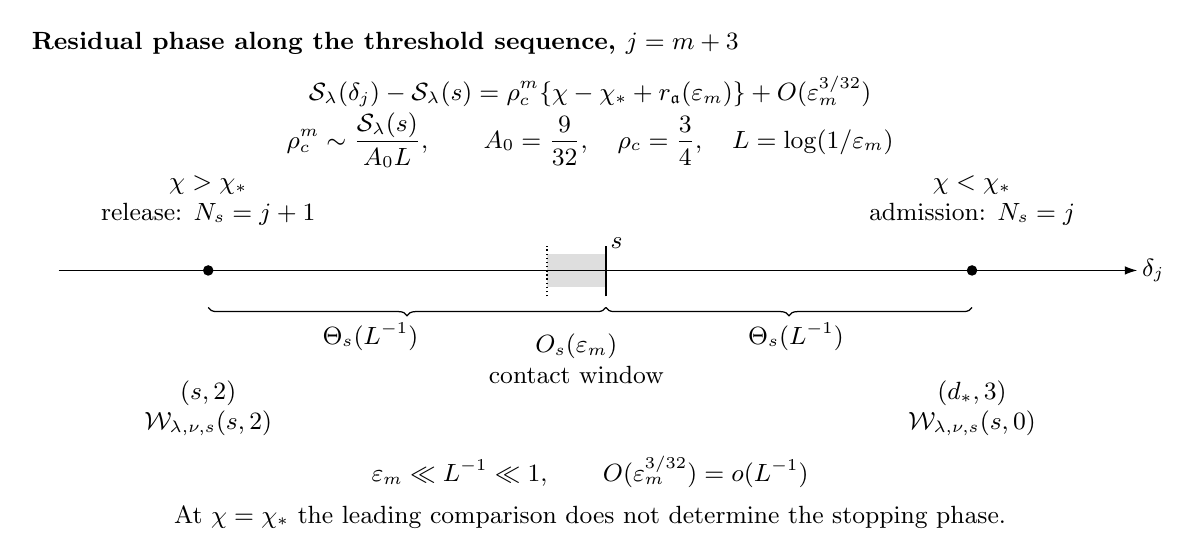
\begin{tikzpicture}[
 x=1cm,y=1cm,font=\small,
 every node/.style={inner sep=1.5pt},
 arrow/.style={-{Latex[length=1.6mm,width=1.1mm]},line width=.5pt},
 brace/.style={decorate,decoration={brace,mirror,amplitude=3pt},
                line width=.45pt}
]
 \node[anchor=west,font=\small\bfseries] at (0,4.80)
   {Residual phase along the threshold sequence, $j=m+3$};
 \node at (7.15,4.18)
   {$\displaystyle \mathcal S_\lambda(\delta_j)-\mathcal S_\lambda(s)
    =\rho_c^m\{\chi-\chi_*+r_{\mathfrak a}(\varepsilon_m)\}
       +O(\varepsilon_m^{3/32})$};
 \node at (7.15,3.56)
   {$\displaystyle \rho_c^m\sim
       \frac{\mathcal S_\lambda(s)}{A_0L},\qquad
       A_0=\frac9{32},\quad\rho_c=\frac34,\quad
       L=\log(1/\varepsilon_m)$};
 \node[align=center] at (2.30,2.80)
   {$\chi>\chi_*$\\release: $N_s=j+1$};
 \node[align=center] at (12.00,2.80)
   {$\chi<\chi_*$\\admission: $N_s=j$};
 \fill[black!13] (6.60,1.70) rectangle (7.35,2.12);
 \draw[arrow] (.40,1.91) -- (14.10,1.91)
   node[right] {$\delta_j$};
 \draw[densely dotted,line width=.5pt] (6.60,1.58) -- (6.60,2.22);
 \draw[line width=.6pt] (7.35,1.58) -- (7.35,2.22);
 \node[above right] at (7.35,2.13) {$s$};
 \fill (2.30,1.91) circle[radius=1.9pt];
 \fill (12.00,1.91) circle[radius=1.9pt];
 \draw[brace] (2.30,1.44) -- (7.35,1.44);
 \draw[brace] (7.35,1.44) -- (12.00,1.44);
 \node at (4.36,1.07) {$\Theta_s(L^{-1})$};
 \node at (9.765,1.07) {$\Theta_s(L^{-1})$};
 \node[align=center] at (6.975,.79)
   {$O_s(\varepsilon_m)$\\contact window};
 \node[align=center] at (2.30,.16)
   {$(s,2)$\\$\mathcal W_{\lambda,\nu,s}(s,2)$};
 \node[align=center] at (12.00,.16)
   {$(d_*,3)$\\$\mathcal W_{\lambda,\nu,s}(s,0)$};
 \node at (7.15,-.65)
   {$\varepsilon_m\ll L^{-1}\ll1,
       \qquad O(\varepsilon_m^{3/32})=o(L^{-1})$};
 \node[align=center] at (7.15,-1.22)
   {At $\chi=\chi_*$ the leading comparison does not determine the stopping phase.};
\end{tikzpicture}
\caption{Residual phase versus contact resolution, with $\lambda,s$
fixed, and $\chi=\chi_\lambda(\mathfrak a)$.
The exact phase decreases with the base, giving opposite signs
for the phase and base gaps. On compact label subclasses separated
from $\chi_*$ by a fixed margin, the base gaps have order $L^{-1}$,
larger than both the comparison error and the necessary contact-stop
window $0<s-\delta_j\le C_s\varepsilon_m$.
The displayed pairs are the actual terminal-pair limits.
The admission-side touchdown is read on the original trajectory
continued past observation. Positions and widths are schematic;
no label attaining $\chi_*$ is assumed.}
\label{fig:selection-mechanism}
\end{figure}


The following two lemmas connect this phase comparison to actual
stopping events and complete path limits.

\begin{lemma}[Identification of an interior contact target]
\label{sel:path-identification}
For fixed labels, if $f_{\eps_m}\to\cW(s,\alpha)$ in $\dF$, with
$0<\alpha<2$, then
$(d_{\eps_m},\alpha_{\eps_m})\to(s,\alpha)$.
\end{lemma}
\begin{proof}
Every subsequence has a further convergent terminal-pair subsequence,
by Theorem~\ref{thm:whole}. If its limit is $(d,\beta)\in\mathcal A_s$,
that theorem gives the path limit $\cW(d,\beta)$.
Ordered convergence preserves endpoints, hence
$\cC_d(\beta)=\cC_s(\alpha)$.
An interior free endpoint has positive normal gap; on contact
$y=z=0$. The two free endpoints are contact admission and release.
The contact endpoint map is injective on $[0,2]$ by
\eqref{gr:contact-injectivity}, including the arrest point $\beta=1$.
An interior contact point is neither admission nor release, so neither
free endpoint nor the repeated admission representation can give this
endpoint. The only possible pair is $(s,\alpha)$, proving convergence
of the full parameter sequence.
\end{proof}

\begin{lemma}[Endpoint test at a fixed touchdown index]
\label{sel:endpoint-test}
Suppose that along a compliance sequence the actual $j$th touchdown
is defined within the common input domain, $j\to\infty$, and
$\delta_j\to s$. If $(\delta_j-s)/\eps\to+\infty$, then
$N_s=j$, the terminal pair tends to $(d_*,3)$ and the ordered path
tends to $\cW_{\lambda,\nu,s}(s,0)$. If
$(\delta_j-s)/\eps\to-\infty$, then $N_s=j+1$, the pair tends
to $(s,2)$ and the path tends to $\cW_{\lambda,\nu,s}(s,2)$.
The index assertions are eventual. All limits, including the
Hausdorff image limits, are uniform on a compact auxiliary class
whenever the hypotheses are uniform there.
\end{lemma}
\begin{proof}
The growth bounds give a positive lower bound for the predecessor
base. Its complete state tends to the graph by
Lemma~\ref{path:stopped-cascade}; the actual return and strict
increase of $F_\lambda$ then give
$\delta_{j-1}\to F_\lambda^{-1}(s)=d_*<s$.
For a positive gap at index $j$, the predecessor contact stays below
the section: its base remains a fixed distance below $s$ and its
contact drift is $O_s(\eps)$. Since $\delta_j>s$, the first
crossing is in its following free flight, before touchdown $j$.
Thus $N_s=j$ and $d_\eps\to d_*$. The unique solution of the
reference section equation at $d_*$ is the free endpoint $3$.

For a negative gap, contact $j$ changes the base coordinate by
$O_s(\eps)$, less than $s-\delta_j$, so it cannot reach the
section. Its input is below the inner cutoffs and has all the
admission margins. Apply the actual return estimate at this input;
its next output tends to $F_\lambda(s)>s$. The first crossing is
in that free flight, with $N_s=j+1$, $d_\eps\to s$ and
$\alpha_\eps>2$. The reference section equation at $s$ has the
unique solution $2$ on $[2,3]$. This use of the next return requires
no iteration at its output.

Strict decrease \eqref{path:strict-p} and the original-prefix
control in Lemma~\ref{path:first-section} exclude earlier crossings.
Theorem~\ref{thm:whole} gives the path limits, using
$\cW(d_*,3)=\cW(s,0)$ at admission. For uniform limits, all base
bounds, contact drifts and complete-state budgets above are uniform.
A varying-label subsequence can have only the stated unique free
root. Match any fixed finite number of last returns uniformly and
put the entire preceding cascade in its common small ball, as in
\eqref{path:whole-error}. The incoming prefix is compared with its
own $I_{\lambda,\nu}$. This gives uniform ordered convergence, and
\eqref{eq:ps5-hausdorff} gives the uniform image convergence.
\end{proof}

\begin{proof}[Proof of Proposition~\ref{sel:threshold-selection}]
Write $L=\log(1/\eps)$. For \textup{(i)}, the exponent in
\eqref{sel:threshold-sequence} strictly decreases to $-\infty$, and
$A_0L=\rho_c^{-m}S_s-\chi_*$. The graph chain started at the actual
$\delta_3^{\mathfrak a}$ has phase at $j=m+3$ equal to
\[
 S_s+\rho_c^m\{\chi_\lambda(\mathfrak a)-\chi_*
                         +r_{\mathfrak a}(\eps_m)\}.
\]
The bounded entrance constants and uniform remainder in
\eqref{sel:uniform-entry-phase} put these graph bases uniformly
near $s$; all bases through $j$ are eventually below $3s/2$.
Lemma~\ref{sel:sharp-phase} therefore continues the actual events
through this same index for every label and gives
\begin{equation}
 \mathcal S_\lambda(\delta_j^{\mathfrak a})-S_s
 =\rho_c^m\{\chi_\lambda(\mathfrak a)-\chi_*
                        +r_{\mathfrak a}(\eps_m)\}
                       +O(\eps_m^{3/32}).
 \label{sel:threshold-phase}
\end{equation}
Here $\rho_c^m\sim S_s/(A_0L)$ and the last error is
$o(\rho_c^m)$. On either compact subclass separated from $\chi_*$
by $\Delta_\chi>0$, the phase difference has the sign of
$\chi_\lambda(\mathfrak a)-\chi_*$ and absolute value between
$c\Delta_\chi\rho_c^m$ and $C\rho_c^m$, uniformly.
Strict decrease and the two-sided Lipschitz bound
\eqref{gr:phase-bilip} give the opposite signed base gap of the
same order. Since $\eps_m=o(\rho_c^m)$,
Lemma~\ref{sel:endpoint-test} proves all index, terminal-pair and
path assertions, including uniformity and image convergence.
Every fixed unequal label belongs to such a separated subclass.
At equality the sign is not determined.

For the event exclusion in \textup{(ii)}, suppose instead that
two fixed unequal labels both stop during contact along a common
sequence tending to zero, at touchdown indices $j_1,j_2$.
The contact window \eqref{eq:contact-stop-location} and the sharp phase
give, for $i=1,2$,
\[
 \rho_c^{j_i-3}
       \{A_0L+\chi_\lambda(\mathfrak a_i)+o(1)\}
                =S_s+O_s(\eps^{3/32}).
\]
Thus $\rho_c^{j_i-3}A_0L\to S_s$. Division gives
$\rho_c^{j_1-j_2}\to1$; because the index difference is an integer,
eventually $j_1=j_2=j$. Subtracting the two equations gives
\[
 \rho_c^{j-3}
 \{\chi_\lambda(\mathfrak a_1)-\chi_\lambda(\mathfrak a_2)+o(1)\}
                   =O_s(\eps^{3/32}).
\]
Multiplication by $L$ contradicts
$\rho_c^{j-3}L\to S_s/A_0>0$ and the unequal constants.
Consequently the exclusion holds below a positive threshold for
this fixed pair. Interior terminal-pair limits eventually give
actual contact stops; Lemma~\ref{sel:path-identification} gives
the same implication for interior ordered-path limits.

For \textup{(iii)}, the identification lemma
puts the $\mathfrak a_0$ stops in contact. Set
$j=N_s^{\mathfrak a_0}-1$. Then
\[
 \delta_j^{\mathfrak a_0}=s+O_s(\eps),\qquad
 \rho_c^{j-3}\sim\frac{S_s}{A_0L}.
\]
For any other fixed $\mathfrak a$, the graph chain started at its
own actual $\delta_3^{\mathfrak a}$ has phase at this index tending
to $S_s$. Its bases through $j$ are eventually below $3s/2$.
The continuation in Lemma~\ref{sel:sharp-phase} therefore compares
the actual events through the same index, even after that
trajectory's observation time. Subtracting the reference relation
gives
\begin{equation}
 \mathcal S_\lambda(\delta_j^{\mathfrak a})-S_s
 =\frac{S_s}{A_0L}
   \{\chi_\lambda(\mathfrak a)
       -\chi_\lambda(\mathfrak a_0)+o(1)\}
       +O_{\mathfrak a,\mathfrak a_0,s}(\eps^{3/32}).
 \label{sel:separation}
\end{equation}
The signed base gap is opposite to the fixed entrance difference
and has size $\Theta(L^{-1})$. Lemma~\ref{sel:endpoint-test} gives
the terminal-pair and ordered-path limits in \textup{(iii)}, with
the stated incoming arcs and image convergence. It is applied at the
index fixed by the reference label, not at the prescribed index of
\textup{(i)}, so no touchdown-count formula for the given sequence is
asserted.
\end{proof}

\begin{proof}[Proof of Theorem~\ref{thm:contact-selection}]
Proposition~\ref{loc:entrance} constructs the entrance constant from
the physical preparation and proves its continuity and boundedness.
The same-index comparison and actual stopping-window estimates lead
to Proposition~\ref{sel:threshold-selection}. Its part
\textup{(ii)} gives assertion \textup{(i)} of the theorem, and
part \textup{(iii)} gives assertion \textup{(ii)}. The common compact classes
and each label's incoming arc are exactly those of
Section~\ref{sec:model}.
\end{proof}

\begin{remark}[Phase and stopping resolution]
\label{sel:criterion}
The integer-index argument uses the following general hypotheses.
Let $L=\log(1/\eps)$, $A>0$, $S_*>0$ and $0<\rho<1$.
Suppose that at the relevant integer event indices
$n\in\mathbb N_0$, for each fixed label $\eta$,
\[
 P_n(\eps,\eta)
   =\rho^n\{AL+\chi(\eta)+r_\eta(\eps)\}+R_n(\eps,\eta),
 \qquad r_\eta\to0,\quad R_n=o(L^{-1}),
\]
where the estimate for $R_n$ is uniform over all relevant event
indices for that fixed label. If the event requires
$|P_n-S_*|\le w_\eta(\eps)=o(L^{-1})$, two fixed labels with
unequal $\chi$ cannot both meet it for arbitrarily small common
$\eps$. The ratio and subtraction argument in the proof of
Proposition~\ref{sel:threshold-selection}\textup{(ii)} applies with
$n_i$ in place of $j_i-3$.
The actual preparation, same-index accuracy and stopping window
needed here were established in Sections~\ref{sec:local-results}
and~\ref{sec:graph}.
\end{remark}

\subsection{Belt ordering of the entrance constant}
\label{sec:entrance-phase}

Theorem~\ref{thm:contact-selection} reduces belt dependence to the
order of the prepared coefficient $C_R$. The following strict order
gives Corollary~\ref{cor:belt-contact-selection}.
Throughout this subsection $\lambda,\theta$ are fixed; the mechanical
coefficient is denoted by $d_\lambda$ as in Section~\ref{sec:model}.

\begin{proposition}[Belt order of the entrance constant]
\label{sel:entrance-phase}
Let $C_R(k)$ be the second-touchdown coefficient in
\eqref{loc:preparation-constants}, and let $K_\lambda$ be the
return coefficient in \eqref{loc:constants}. Then $C_R(k)$ strictly decreases on $I$. Hence
$\chi_{\lambda,\theta}(k)$ in \eqref{sel:chi} strictly increases.
\end{proposition}
\begin{proof}
The normalized critical passage determines $q=q_{\rm in}>0$ from
$(\lambda,\theta)$ alone; see Lemma~\ref{lem:critical-pullback}
and Theorem~\ref{thm:detuned-release}. The normal-release constant
$\nu_\#$ is determined by the fixed linear problem
\eqref{con:canonical-release}, independently of the original labels.
Put $H=ak/\gamma$ and $t=T_f(k)$ in
\eqref{loc:preparation-constants}, where $A_{\rm reb}$ is the
amplitude $A_s$ of \eqref{prep:amplitude}.
Implicit differentiation of the flight equation gives
\[
 t'(k)=-\frac{3\ell(a/\gamma)t}{2ct+3\ell H}<0.
\]
Substitution in the amplitude first yields
\[
 A_{\rm reb}^2=\frac{d_\lambda}{2h^2}
 \left[\gamma Ht^2+(2hc/3+ad_\lambda)t^3\right].
\]
Eliminating $H=(6q-ct^2)/(3\ell t)$ and using
$\gamma=h\ell-d_\lambda$, we obtain
\begin{equation}
 A_{\rm reb}^2=\frac{d_\lambda}{2h^2}
 \left[\frac{2\gamma q}{\ell}t+
 \left(\frac{hc}{3}+\frac{d_\lambda c}{3\ell}+ad_\lambda\right)t^3\right].
 \label{sel:positive-amplitude}
\end{equation}
Every coefficient is positive. Hence the amplitude, $R$ and $C_R$
strictly decrease with $k$, which proves the order of $\chi$.

\end{proof}

The profile dependence requires a different argument, because a
slip level can be visited more than once. We next construct a
single-visit perturbation with nonzero release-speed response.


\begin{proof}[Proof of Corollary~\ref{cor:belt-contact-selection}]
For the exclusion, take $\mathfrak a_i=(k_i,\theta,\nu,\mathbf n)$.
Proposition~\ref{sel:entrance-phase} gives unequal entrance constants
for distinct fixed $k_i$; Proposition~\ref{sel:auxiliary-chi}\textup{(ii)}
therefore gives the event, terminal-pair and ordered-path exclusions.
For a given reference sequence, apply Proposition~\ref{sel:auxiliary-chi}\textup{(iii)} with
$\mathfrak a_0=(k_0,\theta,\nu,\mathbf n)$ and
$\mathfrak a=(k,\theta,\nu,\mathbf n)$. The strict increase of
$\chi_{\lambda,\theta}(k)$ gives admission for $k<k_0$ and release
for $k>k_0$, with the same incoming arc and the corresponding
Hausdorff image convergence.
\end{proof}

\subsection{Friction-profile response}
\label{sec:profile-response}

The belt order does not by itself establish sensitivity to the friction
profile. That question is decided by the normalized critical passage.
A slip level can be visited several times, so a change of the profile
does not provide an independently chosen forcing at each visit.
We use an incoming slip interval visited only once before first release
and prove that its release-speed response cannot vanish in every
admissible direction.

\begin{proposition}[Profile response and entrance order]
\label{sel:profile-response}
Fix a mechanical parameter satisfying the critical-rate and sign
conditions of Section~\ref{sec:model}, and an admissible $C^4$
profile $\Phi^{\rm b}$. Write $q_{\rm in,\lambda}[\Phi]=q_{\rm in}$ for the
normalized first-release velocity in Lemma~\ref{lem:critical-pullback}.
There is $H>Q_\Phi$
such that, for every nonempty open interval $J\subset(H,\infty)$,
there are a nonzero $\psi\in C_c^\infty(J)$ and
$\vartheta_{\max}>0$ for which
\[
 \{\Phi^{\rm b}+\vartheta\psi:
                        |\vartheta|\le\vartheta_{\max}\}
\]
is an admissible compact profile class and
$D_\Phi q_{\rm in,\lambda}[\Phi^{\rm b}](\psi)\ne0$.
Constructing the curve at $\lambda_c=(7/3,0)$, we may orient it
and choose a sufficiently small relative closed mechanical box
$\Lambda_{\rm fr}$ about $\lambda_c$ and a closed parameter interval so that
\begin{equation}
 \partial_\vartheta q_{\rm in,\lambda}[\Phi_\vartheta]\ge c_{\rm fr}>0
 \quad\text{on }\Lambda_{\rm fr}\times
                   [-\vartheta_{\max},\vartheta_{\max}],
 \qquad \Phi_\vartheta=\Phi^{\rm b}+\vartheta\psi.
 \label{sel:profile-local-order}
\end{equation}
For each fixed $\lambda\in\Lambda_{\rm fr}$ and $k\in I$,
$\chi_{\lambda,\vartheta}(k)$ strictly decreases with $\vartheta$.
\end{proposition}
\begin{proof}
On the baseline critical contact write $L=Z-Y$, let $\tau_r$
be its first release, and abbreviate $C=C_G$, $m=\mu A_G$ and
$f=1-\Phi^{\rm b}$. The normalization gives $U\to+\infty$ and
$U'\to-\gamma<0$ as $\tau\to-\infty$. Choose $\tau_0<\tau_r$
with $U'<-\gamma/2$ on $(-\infty,\tau_0]$, and take
\[
 H>\max\{Q_\Phi,\max_{[\tau_0,\tau_r]}U\}.
\]
Every level $u>H$ is visited exactly once before first release;
denote its inverse time by $\tau(u)$.

Let $F_{\Phi^{\rm b}}$ be the contact extension of
\eqref{ent:critical-field}, obtained by replacing $L_+$ by $L$.
In state order $(Y,V,Z,U)$ put
$A(\tau)=D_WF_{\Phi^{\rm b}}(\overline W(\tau))$ and solve
\[
 \zeta'=-A^T\zeta,\qquad
 \zeta(\tau_r)=e_V=(0,1,0,0)^T,\qquad Q=C\zeta_V+m\zeta_U.
\]
For an admissible compactly supported variation,
Lemma~\ref{lem:profile-variation} gives the exact response
\begin{equation}
 D_\Phi q_{\rm in,\lambda}[\Phi^{\rm b}](\psi)
   =-\int_{-\infty}^{\tau_r}LQ\psi(U)\,d\tau.
 \label{sel:profile-adjoint}
\end{equation}
A controllability calculation prevents $Q$ from vanishing on an
interval. Indeed,
\begin{equation}
 \begin{gathered}
 A=A_0+b_0r^T,\qquad
 A_0=\begin{pmatrix}
 0&1&0&0\\0&0&0&0\\1&0&-2&0\\h&0&-h&0
 \end{pmatrix},\\
 b_0=(0,C,0,m)^T,\qquad r=(-f,0,f,f'L)^T,\qquad Q=b_0^T\zeta,
 \\
 \det[b_0,A_0b_0,A_0^2b_0,A_0^3b_0]=-hC^4\ne0.
 \end{gathered}
 \label{sel:profile-controllability}
\end{equation}
If $Q$ vanished on an open contact interval, then
$\zeta'=-A_0^T\zeta$ there. Successive differentiation of
$b_0^T\zeta=0$ would give
$(A_0^jb_0)^T\zeta=0$ for $j=0,1,2,3$.
The determinant in \eqref{sel:profile-controllability} would force
$\zeta=0$, contradicting its nonzero terminal value by linear
uniqueness. Thus $Q$ is not identically zero on any open contact
interval; no analyticity is needed.

Take a nonempty open $J\subset(H,\infty)$. Strict monotonicity,
the mean-value theorem and continuity of the derivative give an open
subinterval where $(\Phi^{\rm b})'>0$. Its time preimage contains
a point with $Q\ne0$. We may therefore choose a closed $K\Subset J$
on which $(\Phi^{\rm b})'$ has a positive lower bound and
$Q(\tau(u))$ has a fixed nonzero sign. Changing variables in
\eqref{sel:profile-adjoint} gives
\[
 D_\Phi q_{\rm in,\lambda}[\Phi^{\rm b}](\psi)
   =-\int_K\frac{L(\tau(u))Q(\tau(u))}{|U'(\tau(u))|}
                   \psi(u)\,du.
\]
A nonzero nonnegative smooth bump supported inside $K$ has nonzero
response. Reverse its sign if needed to make the response positive.

For sufficiently small $|\vartheta|\le\vartheta_{\max}$, the
profile derivative stays positive on $K$, while the profile is
unchanged elsewhere. Its zero, range and saturation limits are
preserved. The core strip and (F3) are unchanged because
$K\subset(Q_\Phi,\infty)$; (F4) holds with a common enlarged
constant since the perturbation has fixed compact support. The
closed parameter curve is continuous in the weighted $C^4$ metric,
and hence compact.

For the common mechanical range choose this curve first at
$\lambda_c$. The model restrictions provide a common mechanical
box for the fixed compact class. Uniform incoming tails give a common
finite time before the support is reached. At each fixed $\lambda$,
all profiles have exactly their baseline's state at that time, so
their shape derivative starts at zero. The baseline state is
continuous in $\lambda$ by Lemma~\ref{lem:critical-pullback}.
Continuous dependence of the finite-time state and linear variation,
together with the transverse first-release event, makes
$\partial_\vartheta q_{\rm in,\lambda}[\Phi_\vartheta]$ jointly continuous
in $(\lambda,\vartheta)$. Its positive value at $(\lambda_c,0)$
gives \eqref{sel:profile-local-order} after restricting the box and
parameter interval. No derivative with respect to $\lambda$ is needed.

Finally keep $\lambda,k$ fixed, put $H_k=ak/\gamma$, and let
$t=t(q)>0$ solve
\[
 ct^2+3\ell H_kt=6q,\qquad t_q=\frac6{2ct+3\ell H_k}>0.
\]
The first amplitude identity in the proof of
Proposition~\ref{sel:entrance-phase} gives
$A_{\rm reb}^2=d_\lambda B(t)/(2h^2)$, where
\[
 B(t)=\gamma H_kt^2+(2hc/3+ad_\lambda)t^3.
\]
As $R=\nu_\#A_{\rm reb}$ and $C_R=\sqrt{6R/c}$,
\begin{equation}
 \partial_q\chi=-\frac3{16}\frac{B'(t)}{B(t)}t_q<0.
 \label{sel:profile-entrance-order}
\end{equation}
Here $\nu_\#$ and $K_\lambda$ are independent of the original
profile. Combining \eqref{sel:profile-local-order} and
\eqref{sel:profile-entrance-order} proves the strict entrance order.
\end{proof}

\begin{corollary}[Friction-profile sensitivity at a fixed belt coefficient]
\label{cor:friction-profile-selection}
Let $\Phi^{\rm b}$ be an admissible $C^4$ baseline profile, and fix
compact belt and physical-preparation classes as in
Section~\ref{sec:model}. There exist a nonzero
$\psi\in C_c^\infty((0,\infty))$, $\vartheta_{\max}>0$, a
sufficiently small relative closed mechanical box $\Lambda_{\rm fr}$
about $\lambda_c=(7/3,0)$, and $s_{\rm fr}>0$ such that
\[
 \Phi_\vartheta=\Phi^{\rm b}+\vartheta\psi,\qquad
 \vartheta\in\Theta_{\rm fr}
              =[-\vartheta_{\max},\vartheta_{\max}]
\]
is a compact class satisfying (F1)--(F4). With this curve as the
profile class, the common model restrictions and
Theorem~\ref{thm:whole} apply on $\Lambda_{\rm fr}$ for
$0<s\le s_{\rm fr}$. Orient the curve so that its normalized
first-release speed $q_{\rm in,\lambda}[\Phi_\vartheta]$ increases with
$\vartheta$ for every $\lambda\in\Lambda_{\rm fr}$.

Fix $\lambda\in\Lambda_{\rm fr}$, $k\in I$, $\nu$, $\mathbf n$
and $0<s\le s_{\rm fr}$. In every system retain
$U_b=U_*-k\sqrt\eps$ and vary only the fixed profile parameter.
\begin{enumerate}[label=\textup{(\roman*)},leftmargin=*]
\item For every two distinct fixed
$\vartheta_1,\vartheta_2\in\Theta_{\rm fr}$
there is $\eps_0>0$, depending on this pair and the fixed data,
such that for $0<\eps<\eps_0$ the two actual first section times
cannot both occur after touchdown and at or before its following
release. Consequently no common sequence $\eps_m\downarrow0$
has terminal-pair limits $(s,\alpha_i)$ for both profiles with
$0<\alpha_i<2$. There is likewise no common sequence with ordered
limits $\cW_{\lambda,\nu,s}(s,\alpha_i)$, even if
$\alpha_1\ne\alpha_2$.
\item Fix $\vartheta_0\in\Theta_{\rm fr}$ and $0<\alpha<2$.
Along any sequence $\eps_m\downarrow0$ for which
$f_{\eps_m}^{(\vartheta_0)}\to\cW_{\lambda,\nu,s}(s,\alpha)$
in $\dF$, every other fixed $\vartheta\in\Theta_{\rm fr}$ satisfies
\[
\begin{array}{c|c|c}
 &\text{terminal pair limit}&\text{ordered-path limit}\\ \hline
 \vartheta>\vartheta_0 &(d_*,3)&\cW(d_*,3)=\cW(s,0)\\
 \vartheta<\vartheta_0 &(s,2)&\cW(s,2).
\end{array}
\]
\end{enumerate}
\end{corollary}

This is the locally constructed profile application of
Theorem~\ref{thm:contact-selection}: the curve and its common
mechanical range are constructed together;
no nonconstancy along a prescribed profile family is assumed.
Each profile is fixed before the compliance limit. With
$\mathbf n=0$ the full physical initial state is the same for all
profiles and compliances, while the belt still follows the stated
joint scaling. Theorem~\ref{thm:whole} supplies the reference
sequences in part \textup{(ii)}; the ordered-path limits also give
the corresponding Hausdorff image convergence by
\eqref{eq:ps5-hausdorff}.



\begin{proof}[Proof of Corollary~\ref{cor:friction-profile-selection}]
Construct the curve at $\lambda_c$ by
Proposition~\ref{sel:profile-response}, choose the common model
range for this compact class, and restrict it as in
\eqref{sel:profile-local-order}. Fix the labels in the corollary.
Equation~\eqref{sel:profile-entrance-order} shows that their entrance
constant strictly decreases with $\vartheta$. Apply
Proposition~\ref{sel:auxiliary-chi}\textup{(ii)} with
$\mathfrak a_i=(k,\vartheta_i,\nu,\mathbf n)$.
Part \textup{(ii)} gives both the terminal-pair and ordered-path
exclusions. For the given reference sequence,
Proposition~\ref{sel:auxiliary-chi}\textup{(iii)} gives admission for
$\vartheta>\vartheta_0$ and release for $\vartheta<\vartheta_0$.
Theorem~\ref{thm:whole} supplies actual reference sequences, and
the same comparison gives Hausdorff image convergence.
\end{proof}

\subsection{Return count and contact-root asymptotics}

\begin{corollary}[Double-logarithmic return count]
\label{sel:return-count}
The actual touchdown count satisfies
\begin{equation}
 N_s(\eps)=\frac{\log\log(1/\eps)}{\log(4/3)}+O_s(1).
 \label{sel:count}
\end{equation}
\end{corollary}
\begin{proof}
The last input belongs to $[c_s,s)$, on which the positive phase
has fixed positive upper and lower bounds. Formula
\eqref{sel:sharp-phase-formula} at $n=N_s-1$ therefore gives
$\rho_c^{N_s-4}L\asymp_s1$. Taking logarithms proves the claim.
\end{proof}

For any actual contact-root family $\eps_j$ with the complete label
fixed, write $C_R=C_R(\lambda,k,\theta)$ and let
$j\to\infty$ be the contact number. The same formula and
\eqref{eq:contact-stop-location} give
\begin{align}
 \log(1/\eps_j)
 &=\tfrac{32}{9}\rho_c^{-(j-3)}\mathcal S_\lambda(s)
       -\tfrac{32}{9}\chi_\lambda(\mathfrak a)+o(1),\nonumber\\
 \eps_j
 &=K_\lambda^{32/3}C_R^{-8/3}
 \exp\{-\tfrac{32}{9}\rho_c^{-(j-3)}\mathcal S_\lambda(s)\}
 (1+o(1)).
 \label{sel:contact-roots}
\end{align}
Indeed $\rho_c^{-(j-3)}=O(L_j)$, so division of the shadow error
costs only $O(L_j\eps_j^{3/32})=o(1)$.
Different interior phases share this asymptotic formula; their
individual selection is supplied by the actual scan of
Lemma~\ref{path:continuous-sweep}.



\section{Observation rules for complete paths}
\label{sec:observations}

Three observation rules act differently on a complete ordered path.
A downstream angle retains a whole contact and a following free prefix;
first hitting the contact angle cuts at admission and is discontinuous
at that path; a fixed local patch crossed strictly by the contact selects
any prescribed interior prefix.

% SCHEMATIC projection of one reference contact to (x=-p/a,Psi).
% Other state coordinates are suppressed. No finite-epsilon contact is drawn.
\begin{figure}[!htbp]
\centering
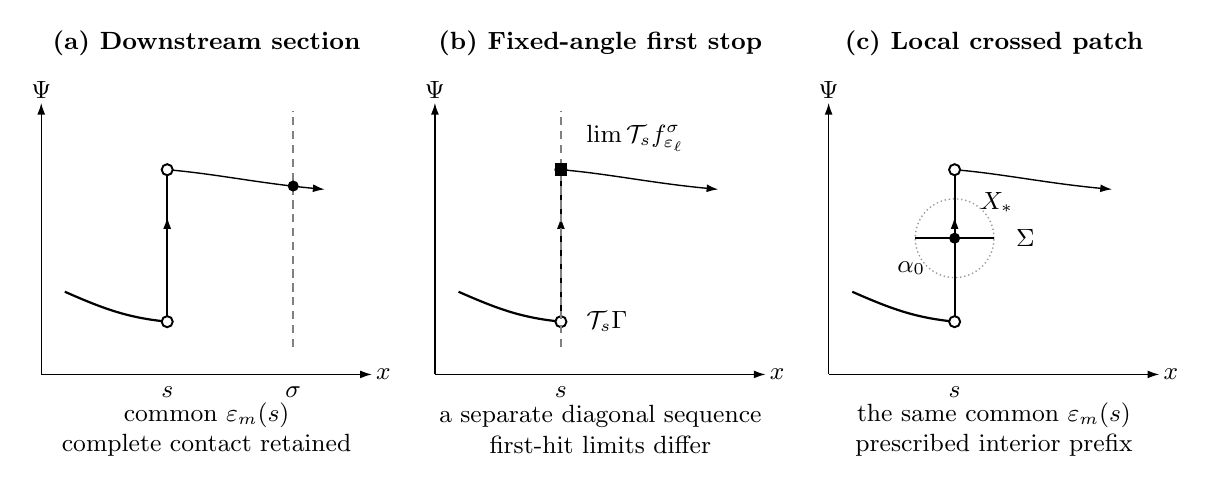
\begin{tikzpicture}[
 x=1cm,y=1cm,font=\small,
 every node/.style={inner sep=1.3pt},
 arrow/.style={-{Latex[length=1.5mm,width=1mm]},line width=.5pt},
 path/.style={draw=black,line width=.8pt},
 section/.style={draw=black!50,densely dashed,line width=.55pt}
]
 \foreach \shift in {0,5.0,10.0}{
  \begin{scope}[xshift=\shift cm]
   \draw[arrow] (.15,.35) -- (4.35,.35) node[right] {$x$};
   \draw[arrow] (.15,.35) -- (.15,3.80) node[above] {$\Psi$};
   \draw[path] (.45,1.40) .. controls (.95,1.18) and (1.25,1.07) .. (1.75,1.02);
   \draw[path] (1.75,1.02) -- (1.75,2.95);
   \draw[arrow] (1.75,1.55) -- (1.75,2.35);
   \draw[path,arrow] (1.75,2.95) .. controls (2.35,2.90) and (2.90,2.78) .. (3.75,2.70);
   \draw[fill=white,line width=.7pt] (1.75,1.02) circle[radius=2pt];
   \draw[fill=white,line width=.7pt] (1.75,2.95) circle[radius=2pt];
   \node[below=3pt] at (1.75,.35) {$s$};
  \end{scope}
 }
 \node[font=\small\bfseries] at (2.25,4.55) {(a) Downstream section};
 \node[font=\small\bfseries] at (7.25,4.55) {(b) Fixed-angle first stop};
 \node[font=\small\bfseries] at (12.25,4.55) {(c) Local crossed patch};
 \draw[section] (3.35,.70) -- (3.35,3.70);
 \node[below=3pt] at (3.35,.35) {$\sigma$};
 \fill (3.35,2.74263) circle[radius=2pt];
 \node[align=center] at (2.25,-.35)
   {common $\varepsilon_m(s)$\\complete contact retained};
 \draw[section] (6.75,.70) -- (6.75,3.70);
 \node[anchor=west] at (7.02,1.02) {$\mathcal T_s\Gamma$};
 \fill (6.67,2.87) rectangle (6.83,3.03);
 \node[anchor=west,align=left] at (7.02,3.35)
   {$\lim\mathcal T_s f_{\varepsilon_\ell}^{\sigma}$};
 \node[align=center] at (7.25,-.35)
   {a separate diagonal sequence\\first-hit limits differ};
 \draw[draw=black!40,densely dotted,line width=.5pt]
   (11.75,2.08) circle[radius=.50cm];
 \draw[line width=.8pt] (11.25,2.08) -- (12.25,2.08);
 \fill (11.75,2.08) circle[radius=2pt];
 \node[anchor=west] at (12.48,2.08) {$\Sigma$};
 \node[anchor=west] at (12.02,2.53) {$X_*$};
 \node[anchor=east] at (11.43,1.70) {$\alpha_0$};
 \node[align=center] at (12.25,-.35)
   {the same common $\varepsilon_m(s)$\\prescribed interior prefix};
\end{tikzpicture}
\caption{Three observations of one limiting contact, schematically
projected to $x=-p/a$ and $\Psi=v-c_\Sigma u_0$
(Corollary~\ref{cor:common-local-contact}), with $s<\sigma<F_\lambda(s)$.
Open circles mark admission and release; arrows indicate curve order.
(a) A downstream section retains the whole contact along the common
sequence $\varepsilon_m(s)$.
(b) The limit path $\Gamma$ first reaches $x=s$ at admission, while
actual first-stop paths from a separate diagonal sequence tend to
release (square).
(c) The fixed local patch crossed strictly at
$X_*=\mathcal C_{\lambda,s}(\alpha_0)$ selects that prefix along the
same sequence as (a). The dotted circle indicates localization only;
the physical patch and its separation from earlier prefixes are
established in full state space. Other coordinates and distinct
incoming arcs are suppressed, not identified.}
\label{fig:observation-rules}
\end{figure}


\subsection{Common paths beyond a complete contact}

Write $f_\eps^\tau$ for the actual path stopped at its first crossing
of $p=-a\tau$, with the same normalization of its parameter interval
as in \eqref{eq:ps5-stop}. The return curve and phase are unchanged. Since $F_\lambda(s)>s$,
there is $s<\sigma\le s_0$ with $\sigma<F_\lambda(s)$ for every
$0<s<s_0$. After a common restriction with $2s\le s_0$ and
$F_\lambda(s)>2s$, one may take $\sigma=2s$.

\begin{corollary}[Common paths beyond a complete contact]
\label{cor:common-downstream-contact}
Fix $\lambda$ and $0<s<\sigma\le s_0$ with
$\sigma<F_\lambda(s)$. The common sequence \eqref{eq:ps5-common}
with target $d=s$ satisfies
\[
 \sup_{(k,\theta,\nu,\mathbf n)}
 \dF\bigl(f_{\eps_m(s)}^\sigma,
  \cW_{\lambda,\nu,\sigma}(s,j_\sigma(s))\bigr)\longrightarrow0.
\]
The corresponding image convergence is uniform in $\dH$.
Here $2<j_\sigma(s)<3$, so the common limiting path includes
the entire contact $\cC_{\lambda,s}|_{[0,2]}$ and a positive-length
prefix of its following free flight.
\end{corollary}

\begin{proof}
The inequalities on $\sigma$ give
$F_\lambda^{-1}(\sigma)<s<\sigma$. Thus $d=s$ is an interior
free target for the $\sigma$ section. Apply
Theorem~\ref{thm:common-free} at that section. Its sequence depends
on $\lambda,d$, but not on the section, so it is precisely
\eqref{eq:ps5-common} with $d=s$. Strict decrease of $p$ along
the free flight and $s<\sigma<F_\lambda(s)$ give
$2<j_\sigma(s)<3$. The flight duration $T_s$ is positive, and
the retained free duration $(j_\sigma(s)-2)T_s$ is therefore positive.
\end{proof}

\subsection{First-angle truncation}

For an oriented path $g:[0,1]\to\R^5$ that starts above and reaches
the section $p=-as$, define its first-hit truncation by
\[
 \mathcal T_s g
   =g|_{[0,\tau_s(g)]},\qquad
 \tau_s(g)=\min\{q\in[0,1]:p(g(q))=-as\},
\]
reparameterized onto $[0,1]$. This operation is well defined in the
zero-distance quotient of \eqref{eq:ps5-frechet}. Indeed, two
zero-distance paths admit a common representation
$g\circ a=\widetilde g\circ b$, with $a,b$ continuous
nondecreasing surjections. Such a representation is obtained by
taking a limit of the increasing comparison graphs and
parameterizing the limiting monotone relation by the sum of its
coordinates. At the first section
point of the common representation, $a$ and $b$ reach the first
section parameters of $g$ and $\widetilde g$, respectively.
Restricting $a,b$ there gives a common representation of their
prefixes. Thus only inserted pauses can differ, and the prefixes
have zero ordered distance.

\begin{corollary}[Discontinuity of first-hit truncation]
\label{cor:first-hit-discontinuity}
Under the same restrictions on $\lambda,s,\sigma$, fix a complete
label $\mathfrak l=(\lambda,k,\theta,\nu,\mathbf n)$ and put
\[
 \Gamma=\cW_{\lambda,\nu,\sigma}(s,j_\sigma(s)).
\]
There is a sequence $\eps_\ell\downarrow0$ for this label such that
\[
 \begin{split}
 \dF(f_{\eps_\ell}^\sigma,\Gamma)&\longrightarrow0,\\
 \dF(\mathcal T_s f_{\eps_\ell}^\sigma,
       \cW_{\lambda,\nu,s}(s,2))&\longrightarrow0,
 \end{split}
\]
whereas
$\mathcal T_s\Gamma=\cW_{\lambda,\nu,s}(s,0)$ in the ordered
quotient. These two stopped limit paths have different endpoints.
Consequently $\mathcal T_s$ is discontinuous at $\Gamma$, even on
the subspace consisting of $\Gamma$ and actual paths stopped at
the $\sigma$ section.
\end{corollary}

\begin{proof}
Choose $d_\ell\uparrow s$ with
$F_\lambda^{-1}(\sigma)<d_\ell<s$. Each $d_\ell$ is an interior
free target for both the $s$ and $\sigma$ sections. The explicit
sequences supplied by Theorem~\ref{thm:common-free} at these two
sections are identical:
\[
 \eps_m(d_\ell)=
 \exp\{-\tfrac{32}{9}(3/4)^{-m}\mathcal S_\lambda(d_\ell)\}.
\]
For each $\ell$, take $m_\ell$ sufficiently large that both
ordered-path errors are below $1/\ell$, and also that
$\eps_{m_\ell}(d_\ell)<1/\ell$ and, when $\ell>1$,
$\eps_{m_\ell}(d_\ell)<\eps_{m_{\ell-1}}(d_{\ell-1})/2$.
Write $\eps_\ell=\eps_{m_\ell}(d_\ell)$.

Continuous dependence of the finite-scale return curves and their
free-section roots gives
\[
 j_\sigma(d_\ell)\longrightarrow j_\sigma(s),\qquad
 j_s(d_\ell)\longrightarrow j_s(s)=2.
\]
The complete-path continuity proved after
\eqref{path:whole-error}, applied separately at the fixed sections
$s$ and $\sigma$, therefore gives
\[
 \begin{split}
 \cW_{\lambda,\nu,\sigma}(d_\ell,j_\sigma(d_\ell))
      &\longrightarrow\Gamma,\\
 \cW_{\lambda,\nu,s}(d_\ell,j_s(d_\ell))
      &\longrightarrow\cW_{\lambda,\nu,s}(s,2).
 \end{split}
\]
The two diagonal error bounds prove the two asserted actual limits.
The actual $s$ section is reached before the $\sigma$ section,
and its prefix is exactly
$\mathcal T_s f_{\eps_\ell}^\sigma=f_{\eps_\ell}^s$ in the
ordered quotient.

The incoming arc has $p\ge0$. Every return preceding the base $s$
in $L_s$ has $p>-as$ except that the last reaches $-as$ at its
final touchdown, the admission point $\cC_{\lambda,s}(0)$.
Hence $\Gamma$ first reaches this section at that admission point,
and its first-hit prefix is $\cW_{\lambda,\nu,s}(s,0)$.
The admission slip is $U_s>0$ from \eqref{gr:embedding}, while
the release slip is zero. In particular,
\[
 |\cC_{\lambda,s}(2)-\cC_{\lambda,s}(0)|
   \ge \frac{U_s}{|\cos\phi_s|}>0.
\]
The ordered distance bounds the distance between terminal states,
so the limits of the truncated paths and of the long paths cannot
commute. This proves the claimed discontinuity.
\end{proof}

\subsection{Fixed local observation patches}

The angular section contains the whole limiting contact. A local patch
can cross it at any prescribed interior point: the next construction
uses slip on compression, normal velocity on release, and the two
one-sided crossings at arrest.

\begin{corollary}[Common contact prefixes at a local observation surface]
\label{cor:common-local-contact}
Fix $\lambda$, $0<s<\sigma\le s_0$ with
$\sigma<F_\lambda(s)$, and $\alpha_0\in(0,2)$. Put
\[
 X_*=\cC_{\lambda,s}(\alpha_0),\qquad
 h_s=\mu A(\phi_s)-B(\phi_s)>0,
\]
and choose $c_\Sigma>as/h_s$. Define on physical states
\[
 u_0(\cX)=\omega\cos\phi+U_*,\qquad
 \Psi(\cX)=v-c_\Sigma u_0(\cX).
\]
There is $r_\Sigma>0$ such that the closed observation patch
\[
 \Sigma=\{\cX:|\cX-X_*|\le r_\Sigma,\quad
                         \Psi(\cX)=\Psi(X_*)\}
\]
has the following property. For all sufficiently large $m$, every
actual trajectory at $\eps=\eps_m(s)$ in the prescribed compact auxiliary label class
first meets $\Sigma$ before reaching $p=-a\sigma$, and this first
meeting occurs during the actual contact whose base tends to $s$.
If $f_\eps^\Sigma$ is the path stopped at this first meeting and
reparameterized onto $[0,1]$, then
along the common sequence \eqref{eq:ps5-common} with $d=s$,
\[
 \sup_{(k,\theta,\nu,\mathbf n)}
 \dF\bigl(f_{\eps_m(s)}^\Sigma,
             \cW_{\lambda,\nu,s}(s,\alpha_0)\bigr)
       \longrightarrow0.
\]
The image convergence is also uniform in $\dH$. The patch is
independent of $\eps$ and the auxiliary labels; each incoming datum
retains its own arc $I_{\lambda,\nu}$.
\end{corollary}

\begin{proof}
The exact contact formulas \eqref{gr:embedding} and
\eqref{eq:ps2-reference-path} give, on compression,
\[
 \frac{\dd}{\dd\alpha}\Psi(\cC_{\lambda,s}(\alpha))
       =(c_\Sigma-as/h_s)U_s>0\qquad(0<\alpha<1).
\]
On release $u_0=0$, and \eqref{loc:normal-reference} gives
\[
 \frac{\dd}{\dd\alpha}\Psi(\cC_{\lambda,s}(\alpha))
   =\tfrac12s^{3/2}R_s
      (Z_s-Y_s)((\alpha-1)R_s)>0\qquad(1<\alpha<2).
\]
The active force is positive before its first zero. These two
formulas and the continuous join show that $\Psi$ is strictly
increasing along the entire reference contact. At $\alpha_0=1$
we use the two one-sided strict crossings.

The compact tail $L_s$ meets $p=-as$ only at
$\cC_{\lambda,s}(0)$, whose $\Psi$ value is smaller than
$\Psi(X_*)$. Hence $X_*\notin L_s$. Choose $r_\Sigma>0$ so that the
closed $2r_\Sigma$ ball about $X_*$ avoids $L_s$ and is contained in
$\{p<0\}$. Every incoming arc lies in $\{p\ge0\}$, so this
choice also separates the patch from all incoming arcs uniformly.

Choose $\eta>0$ with
$0<\alpha_-:=\alpha_0-\eta<\alpha_+:=\alpha_0+\eta<2$
so small that $\cC_{\lambda,s}([\alpha_-,\alpha_+])$
lies in the open $r_\Sigma$ ball. At the two ends $\Psi-\Psi(X_*)$
has opposite signs. The earlier contact segment
$\cC_{\lambda,s}([0,\alpha_-])$ has strictly smaller
$\Psi$ value and is a positive distance from the closed patch.
Together with the preceding tail and incoming-arc separation,
this gives a uniform positive distance between $\Sigma$ and
the entire preceding reference prefix.

Corollary~\ref{cor:common-downstream-contact} and its ordered
pairings give uniform convergence of the actual paths through
this contact. More specifically,
Lemma~\ref{path:ordered-return} pairs its compression and release
with $\cC_{\lambda,s}|_{[0,2]}$, after using the convergence of
the actual base to $s$. These pairings align the earlier prefixes
as in the proof of Theorem~\ref{thm:whole}. Thus, for large $m$,
the actual trajectory cannot meet $\Sigma$ before the paired
point $\alpha_-$, while the whole paired bracket stays in the
open $r_\Sigma$ ball and its end values of $\Psi-\Psi(X_*)$ have opposite
signs. The intermediate value theorem supplies a meeting inside
this bracket. Since $\Sigma$ is closed, the nonempty set of
meeting times up to the end of the bracket is compact and has a
first element. It lies between the paired points $\alpha_-$
and $\alpha_+$, within this actual contact.

Restrict the ordered pairings at that first meeting. Their
errors tend to zero uniformly in the auxiliary labels, and the
reference stopping parameter lies in
$[\alpha_0-\eta,\alpha_0+\eta]$. Uniform continuity of
$\cC_{\lambda,s}$, followed by $\eta\downarrow0$, proves the
asserted prefix convergence. The image assertion follows from
$\dH\le\dF$.
\end{proof}

Appendix~\ref{sec:accumulation-geometry} identifies the single
terminal-parameter duplication and proves that the full-state accumulation
families are circles. Appendix~\ref{sec:memory} records the interval of
scaled effective-gap velocities above the release endpoint path.

\section{Discussion}
\label{sec:discussion}

The selection comparison uses three inputs: an entrance phase with
a bounded correction and a uniform vanishing remainder, a same-index
return error smaller
than $1/\log(1/\eps)$, and localization of the actual stopping
event to a narrower window. Together they explain why parameter
dependence disappears for a free target but determines on which
side of a contact the first crossing occurs. The abstract criterion
in Remark~\ref{sel:criterion} records this last comparison;
the original preparation, admissible return domains and sharp
full-state budget establish its hypotheses here. For complete
paths one also needs convergence of the incoming motion, ordered
comparison of any fixed number of final returns, and a common
shrinking neighborhood for the whole earlier tail.

The normal filter, the $3/4$ return exponent, the $9/32$ entrance
exponent and the signs ordering $\chi$ come from the specified
mechanical and constitutive laws. Compactly supported profile
variations share an exact incoming tail, so their critical-passage
response reduces to a finite-time variational problem
(Lemma~\ref{lem:profile-variation}). Controllability and the
single-visit high-slip interval then supply a direction with nonzero
response, with a common mechanical box and section chosen for the
constructed compact curve. The profile tails and mechanical rate
margins also enter the preparation estimates. The prescribed compact $\beta$ range makes the preparation
estimates uniform; it is the range treated by the present proof.
The signed first contact permits $r=O(\delta)$, whereas the
preparatory flights put later inputs in $r\le A\delta^{4/3}$.
A different detuning scale or normal law would require its own
entrance and return estimates before the selection comparison
could be applied.

The observation results distinguish a longer path from the first
fixed-angle prefix that it contains. A strict local crossing gives
continuous prefix selection, while the angle section contains the
whole limiting contact and has a discontinuous first-hit operation.
The additional scaled-memory and path-identification results retain
information that can be lost by projecting the state or discarding
the contact order.

The selection results compare fixed labels. Whether belt or profile
parameter differences of order $\eps\log(1/\eps)$ yield a transition
law remains open. The absolute shadowing estimate used here does
not control such parameter increments.

\appendix
\section{From physical preparation to the first release}
\label{sec:entry}
The incoming normal equilibrium loses uniform attraction as $p$ tends
to zero. Negative detuning moves the relevant slip transition to
$p\asymp\sqrt\eps$, where normal dissipation and variation of its
energy metric have comparable sizes. We follow the prescribed rigid
trace by coupling a normal energy with its exact weak coefficient.
A first graph correction has identically zero force defect. The
resulting energy estimate controls the outer range by dissipation and
the critical annulus by a bounded Gronwall factor. Although the weak
coefficient loses accuracy there, conversion back to the physical
state multiplies its error by $p^\beta$. This gives the complete
normal state needed for the first release.

The compact classes are those of Section~\ref{sec:model}. In particular,
$r=-\eta=k\sqrt\eps$, $k\in I=[k_-,k_+]\Subset(0,\infty)$,
and all labels, including the original fast triple, are fixed before
$\eps\downarrow0$. Constants below are common on these classes.
Write $\gamma=-g_*>0$ and $\rho=b/p$.

\subsection{The weak coordinate and a finite normal energy}

\paragraph{The rigid first integral.}
Let $\alpha_1=F_{\rm free}p$, $\alpha_2=F_{\rm free}b$ and
$\alpha_3=-Q_{\rm sat}b$, restricted to $y=v=0$ when written as
functions of $(p,b)$. The rigid saturated field is
\begin{equation}
 \begin{gathered}
 \dot p=\alpha_1,\qquad \dot b=\alpha_2+\alpha_3b/p,\\
 F(p,\rho)=\frac{\alpha_2+(\alpha_3-\alpha_1)\rho}{p},\qquad
 \mathscr D=\alpha_1\partial_p+F\partial_\rho.
 \end{gathered}
 \label{ent:rigid-field}
\end{equation}
Here $\alpha_1(G)=-a$, $\alpha_2(G)=-c$,
$\alpha_3(G)=-a\beta$ and $c=a(\beta-1)\ell$.
The scalar equation for $\rho$ has the regular-singular form
\[
 p\rho_p=H(p,\rho),\qquad
 H=\frac{\alpha_2(p,p\rho)+(\alpha_3-\alpha_1)(p,p\rho)\rho}
              {\alpha_1(p,p\rho)},\qquad
 H(0,\rho)=(\beta-1)(\rho+\ell).
\]
To construct its analytic weak curve, put $s=\bar\rho+\ell$.
Its equation is $(p\partial_p-(\beta-1))s=pJ(p,s)$, with $J$
analytic. In absolutely convergent power series the inverse diagonal
operator divides coefficient $n$ by $n-(\beta-1)$, $n\ge1$.
These divisors stay away from zero uniformly for
$2<\beta_-\le\beta\le\beta_+<5/2$. On a sufficiently small common
disk multiplication by $p$ therefore makes the fixed-point equation
for $s$ a contraction. This gives $\bar b=p\bar\rho=-\ell p+O(p^2)$.

For $d_b=\rho-\bar\rho$, subtraction gives exactly
$d_b'=((\beta-1)/p+A_0(p,d_b))d_b$, where $A_0$ is analytic
and bounded: $\partial_\rho H-(\beta-1)$ is divisible by $p$.
Thus $d_b=p^{\beta-1}\zeta$ satisfies
$\zeta'=A_0(p,p^{\beta-1}\zeta)\zeta$, a regular equation down
to $p=0$ on each bounded $\zeta$ set. Define $\mathcal C(p,b)$
as its limiting value there. Its integral equation and variational
equation give
\begin{gather}
 b(p,C)=\bar b(p)+p^\beta\{C+O(p)\},\qquad
 |\nabla_{p,b}\mathcal C|\le Cp^{-\beta},\notag\\
 |b(p,C)-b(p,\widetilde C)|\le Cp^\beta|C-\widetilde C|,
 \label{ent:weak-coordinate}\\
 \rho=-\ell+O(p)+O(p^{\beta-1}),\qquad
 \mathscr D\rho=O(1),\qquad
 \mathscr D^2\rho=O(p^{\beta-3}).
 \label{ent:weak-derivatives}
\end{gather}
For the first line, the variation in $\zeta$ and its inverse are
bounded by $e^{Cp}$; conversion from
$\zeta=(b-\bar b)/p^\beta$ gives the displayed derivatives.
For the second, differentiate the regular equation along the rigid
field. These are values of rigid derivatives at points of a bounded
coefficient wedge, not derivatives of an actual fast transient.
In particular $|F_p|+|F_\rho|\le C/p$ there. The exact first
integral equals the prescribed $C_1$ on the prescribed rigid trace.

\paragraph{A degenerating normal energy.}
The normal decay rate tends to zero with $p$. We therefore seek a
Lyapunov norm whose square decays at a rate proportional to $p$ for
the frozen normal equation in fast time. Converting this norm to
displacement and memory will cost
$p^{-1/2}$, whereas the velocity estimate remains uniform. These
component weights determine how the normal error enters the weak
coordinate estimate below.

Set $N=(Y,V,Z)=(y/\eps^2,v/\eps,z/\eps^2)$ and define
\begin{equation}
 M_o(p)=\begin{pmatrix}0&1&0\\-p&0&p\\1&0&-2\end{pmatrix},\quad
 e_{\rm eq}=(2,0,1)^T,\quad q_N=(-1,0,1)^T,\quad a_1=(-1,2,-1)^T.
 \label{ent:normal-matrix}
\end{equation}
The polynomial of $M_o$ is $z^3+2z^2+pz+p$.
Its simple root $f=-2+p/4+O(p^2)$ is analytic; write the remaining
factor as $z^2-a_cz+d_c$, where
$a_c=-p/4+O(p^2)$ and $d_c=p/2+O(p^2)$. The polynomial projector
\[
 \begin{gathered}
 P_f=\frac{M_o^2-a_cM_o+d_cI}{f^2-a_cf+d_c},\qquad P_c=I-P_f,\\
 c_2=P_c(0,2,-1/2)^T,\quad c_1=(M_o-a_cI)c_2,\quad
 e_f=P_f(0,0,1)^T.
 \end{gathered}
\]
defines an analytic invertible matrix $T_o=(c_1,c_2,e_f)$.
At zero its columns are $e_{\rm eq}$, $(0,2,-1/2)^T$ and $(0,0,1)^T$;
their determinant is $4$, and
\[
 T_o^{-1}M_oT_o=\operatorname{diag}(A_c,f),\qquad
 A_c=\begin{pmatrix}0&1\\-d_c&-h_c\end{pmatrix},\qquad h_c=-a_c.
\]
Put $S_c=\left(\begin{smallmatrix}d_c&h_c/2\\h_c/2&1\end{smallmatrix}\right)$
and $\mathbb S=T_o^{-T}\operatorname{diag}(S_c,1)T_o^{-1}$.
The exact identity $A_c^TS_c+S_cA_c=-h_cS_c$ and $f<-1$ give
\begin{equation}
 \begin{gathered}
 M_o^T\mathbb S+\mathbb SM_o\le-c_0p\mathbb S,\\
 |w_1|+|w_3|+|q_N^Tw|\le Cp^{-1/2}W,\qquad |w_2|\le CW,
 \end{gathered}
 \label{ent:energy-weights}
\end{equation}
where $W=\|w\|_{\mathbb S}$; also
$\|e_{\rm eq}\|_{\mathbb S}\le C\sqrt p$ and
$\|a_1\|_{\mathbb S}+\|(0,1,0)^T\|_{\mathbb S}\le C$.
Indeed $S_c\asymp\operatorname{diag}(p,1)$; the first and third
columns of $T_o$ have second component $O(p)$, giving the stronger
$w_2$ bound. To differentiate the metric, write
$D_o=\operatorname{diag}(S_c,1)$, $\zeta_o=T_o^{-1}w$ and
$B_o=T_o^{-1}T_o'$. Then
\[
 w^T\mathbb S'w=\zeta_o^TD_o'\zeta_o
 -\zeta_o^T(B_o^TD_o+D_oB_o)\zeta_o,
 \qquad |w^T\dot{\mathbb S}w|\le C|\dot p|p^{-1}W^2.
\]
This estimate uses the actual $\dot p$.

\paragraph{Coupled tracking of the normal and weak coordinates.}
The first graph correction is
\begin{equation}
 G_1=\eps a_1F,\qquad N=e_{\rm eq}\rho+G_1+w.
 \label{ent:first-graph}
\end{equation}
It satisfies $M_oG_1=\eps e_{\rm eq}F$ and $q_N^TG_1=0$ exactly.
To keep the finite-profile feedback, evaluate $A_j=\alpha_j$
at the actual mechanical state
$\Xi(p,p\rho,\eps^2(2\rho+G_{1,1}+w_1),\eps(G_{1,2}+w_2))$,
and set
\[
 \begin{gathered}
 d_\eps=\{A_2+(A_3-A_1)\rho\}/p,\qquad
 \mathcal T_v=\mu B(1-\Phi_\theta(u/\eps))\lambda_N,\\
 \mathcal T_b=\mu(1-\Phi_\theta(u/\eps))\lambda_N
                      (\partial_{\dot q}b)M^{-1}Q_T.
 \end{gathered}
\]
With $E=G_1+w$ the exact equations are
\begin{align*}
 \dot p&=A_1,&
 \dot\rho&=d_\eps-(A_3/p)q_N^TE+\mathcal T_b/p,\\
 \eps\dot E&=M_oE-\eps e_{\rm eq}d_\eps+
       \eps(A_3/p)e_{\rm eq}q_N^TE+\mathcal T_ve_V-\eps e_{\rm eq}\mathcal T_b/p,
 &&e_V=(0,1,0)^T.
\end{align*}
Subtracting the derivative of $G_1$ gives, without truncation,
\begin{equation}
 \begin{split}
 \eps\dot w={}&M_ow+\eps\frac{A_3}{p}(e_{\rm eq}+G_{1,\rho})q_N^Tw\\
 &-\eps(e_{\rm eq}+G_{1,\rho})(d_\eps-F)-\eps G_{1,p}(A_1-\alpha_1)
 -\eps^2a_1\mathscr D^2\rho\\
 &\phantom{{}={}}
 +\mathcal T_ve_V-\frac\eps p(e_{\rm eq}+G_{1,\rho})\mathcal T_b.
 \end{split}
 \label{ent:exact-remainder}
\end{equation}
In particular both profile terms remain in the normal equation.

Here are the estimates needed to use this identity. They hold for
$p\ge h\sqrt\eps$, with any fixed $h>0$, on partial intervals with
bounded weak coefficient, strict normal-force bounds,
$W\le\rho_0\sqrt p$, and $a/2\le-\dot p\le2a$.
From \eqref{ent:weak-derivatives},
$G_1=O(\eps)$,
$\|G_{1,p}\|_{\mathbb S}+\|G_{1,\rho}\|_{\mathbb S}\le C\eps/p$,
and $\|e_{\rm eq}+G_{1,\rho}\|_{\mathbb S}\le C_h\sqrt p$.
The last bound uses $\eps/p^{3/2}\le h^{-3/2}\eps^{1/4}$.
Superscript $G$ denotes $w=0$. Since its physical $y,v$ are
$O(\eps^2)$, $|A_j^G-\alpha_j|\le C\eps^2$ and
$|d_\eps^G-F|\le C\eps^2/p$.
The four saturated inhomogeneous terms in
\eqref{ent:exact-remainder} have energy bounds, respectively,
\begin{equation}
 C\eps^2p^{\beta-3},\qquad C\eps^3p^{-1/2},\qquad
 C\eps^4p^{-2},\qquad C\eps^4p^{-1},
 \label{ent:forcing-domination}
\end{equation}
when ordered as $-\eps^2a_1\mathscr D^2\rho$,
$-\eps e_{\rm eq}(d_\eps^G-F)$,
$-\eps G_{1,\rho}(d_\eps^G-F)$ and
$-\eps G_{1,p}(A_1^G-\alpha_1)$.
Relative to $\eps^2p^{\beta-3}$, the last three bounds have ratios
$\eps p^{5/2-\beta}$, $\eps^2p^{1-\beta}$ and
$\eps^2p^{2-\beta}$. For $h\sqrt\eps\le p\le p_i<1$ and the
prescribed compact range $\beta<5/2$, these are uniformly small.
Thus each term is bounded by $C_h\eps^2p^{\beta-3}$.
At $\beta=5/2$ these three ratios are, respectively,
$O(\eps)$, $O_h(\eps^{5/4})$ and $O_h(\eps^{7/4})$ on the same
interval. These bounds describe the endpoint of this forcing
calculation; the proof below uses the prescribed compact range.
The physical differences from this graph are
$(\eps^2w_1,\eps w_2)$, so
$|A_j-A_j^G|\le C\eps W$ and
$|d_\eps-d_\eps^G|\le C\eps W/p$.
The three homogeneous terms have bounds
$C_h\eps W/p$, $C_h\eps^2p^{-1/2}W$ and
$C\eps^3W/p$. A value bound $1-\Phi_\theta(u/\eps)\le CR_\Phi$
gives for the complete profile forcing
$C_hR_\Phi(1+\eps p^{-1/2}+\eps^2p^{-2})\le C_hR_\Phi$.
The metric derivative and \eqref{ent:energy-weights} consequently give
\begin{equation}
 \eps D^+W\le(-c_0p+C_h\eps/p)W
                +C_h\eps^2p^{\beta-3}+C_hR_\Phi.
 \label{ent:signed-energy}
\end{equation}
We retain the positive metric term when crossing the critical annulus.
Finally the rigid field annihilates $\mathcal C$. At equal $(p,b)$,
its difference from the actual field is
\[
 \delta\dot p=A_1-\alpha_1,\quad
 \delta\dot b=(A_2-\alpha_2)+(A_3-\alpha_3)\rho
                         -A_3q_N^Tw+\mathcal T_b,
 \quad |A_j-\alpha_j|\le C(\eps^2+\eps p^{-1/2}W).
\]
Thus \eqref{ent:weak-coordinate} yields the coupled transport bound
\begin{equation}
 \left|\frac{d\mathcal C_\eps}{dp}\right|
 \le C\{\eps^2p^{-\beta}+p^{-\beta-1/2}W+R_\Phi p^{-\beta}\}.
 \label{ent:weak-transport}
\end{equation}

\subsection{Capture and the actual descending threshold}

\begin{lemma}[The actual incoming threshold]\label{lem:detuned-threshold}
The physical initial states reach a common fixed section $p=p_i>0$
in positive-slip contact. On its continuous contact passage there is a
unique first descending crossing $t_e$ of $u(t_e)=\gamma\eps T$,
where $T=m|\log\eps|$ and $m$ is a sufficiently large fixed constant.
If $p_{\rm stop}$ is the zero of the prescribed detuned rigid slip,
then
\begin{gather}
 p_{\rm stop}=ak\sqrt\eps/\gamma+O(\eps),\qquad
 p_e=p_{\rm stop}+a\eps T+R_e,\qquad R_e=o(\eps),
 \label{ent:threshold-slow}\\
 b_e=-\ell p_{\rm stop}+o(\sqrt\eps),\quad
 |X_e-G|=O(\sqrt\eps),\quad
 \lambda_N(t_e)=\ell+O(\sqrt\eps),\quad V_e=O(\eps),\\
 E_{N,e}:=|Y_e+2\ell|+|V_e|+|Z_e+\ell|=O(\sqrt\eps).
 \label{ent:threshold-normal}
\end{gather}
All assertions are uniform on the fixed compact classes.
\end{lemma}
\begin{proof}
For capture, freeze $p>0$, $b<0$ on a closed incoming rigid arc and
put $\ell_f=-b/p$. The frozen fast equations and proper energy are
\[
 \begin{gathered}
 Y'=V,\quad V'=b+pL,\quad Z'=-Z-L,\quad L=(Z-Y)_+,
 \\
 \mathcal E_f=\frac{V^2}{2p}+\frac{Z^2+L^2}{2}+\ell_fY,
 \qquad \mathcal E_f'=-(Z')^2.
 \end{gathered}
\]
Minimization over $Z$ gives potential $\ell_fY$ for $Y\ge0$ and
$Y^2/4+\ell_fY$ for $Y<0$, so sublevels are uniformly compact
on the fixed positive ranges of $p,\ell_f$. In an invariant
zero-dissipation set, $L=-Z$. If $L>0$, then $Y=2Z$, $V=0$,
and $V'=0$ gives $L=\ell_f$; if $L=0$, then $Z=0$, $Y\ge0$,
but $Y''=b<0$ cannot remain there. The invariance principle therefore
gives attraction to $(-2\ell_f,0,-\ell_f)$, including initially
free states. The Hurwitz matrix \eqref{ent:normal-matrix} gives a
common local exponential estimate on this fixed arc. Continuous
dependence and a finite cover of the parameter and initial-state
compact sets give a common finite fast capture time. Over it the
actual slow drift is $O(\eps)$ and the closed-arc slip margin makes
the profile error $O(e^{-c/\eps})$, so the actual trajectory enters
the strict-contact neighborhood too.

Subtract the moving equilibrium there. Its physical-time derivative
is bounded on the fixed arc; the local Lyapunov inequality gives
$|N-N_*(p,b)|\le Ce^{-c(t-t_c)/\eps}+C\eps$.
The time integral of the slow-field discrepancy is $O(\eps)$.
Gronwall and alignment at a transverse section, leaving a fixed
positive time after capture, give
\begin{equation}
 \mathcal C_\eps(p_i)=C_1+O(\eps),\quad W(p_i)=O(\eps),\quad
 t_\eps(p_i)-t_{{\rm rig},\nu}(p_i)=O(\eps).
 \label{ent:fixed-initialization}
\end{equation}
The graph correction is $O(\eps)$ at this section. Capture before it
may contain departures and recontacts.

We now stop on partial intervals by
$|\mathcal C_\eps-C_1|\le1$, $W\le\rho_0\sqrt p$, strict force
bounds, the regular chart and $a/2\le-\dot p\le2a$, adding the
slip bounds below. Choose $p_i,\rho_0$ small, then $K_L$ large,
and finally $\eps$ small. On $p\ge K_L\sqrt\eps$ the positive
term in \eqref{ent:signed-energy} is absorbed, and the rigid slip
slope is $\gamma/a$. Requiring $u\ge c_{\rm sl}p$ gives a profile
tail smaller than every fixed power of $\eps$. Integration in the
actual decreasing $p$ direction gives
\begin{equation}
 W(p)\le H_\eps(p)+C\eps^2p^{\beta-4}+CR_\Phi/p,\qquad
 H_\eps=CW(p_i)e^{-c(p_i^2-p^2)/\eps}.
 \label{ent:safe-tracking}
\end{equation}
Indeed the forcing integral is
$C\eps\int_p^{p_i}e^{-c(s^2-p^2)/\eps}s^{\beta-3}\,ds$;
$s^2-p^2\ge2p(s-p)$ bounds it by $C\eps^2p^{\beta-4}$.
Substitution into \eqref{ent:weak-transport} gives
\begin{equation}
 |\mathcal C_\eps(p)-C_1|\le
 C\{\eps+\eps^2p^{1-\beta}+\eps^2p^{-7/2}
                           +R_\Phi p^{-\beta-1/2}\}.
 \label{ent:coefficient-bound}
\end{equation}
The principal transport integral is
$\eps^2\int_p^{p_i}s^{-9/2}\,ds=O(\eps^2p^{-7/2})$.
The weighted integral of $H_\eps$ is $O(\eps W(p_i))=O(\eps^2)$:
above $p_i/2$ its width is $O(\eps)$, and below $p_i/2$ the fixed
exponential absorbs every endpoint power. Thus the safe endpoint has
$W=O(\eps^{\beta/2})$ and $\mathcal C_\eps-C_1=O(\eps^{1/4})$.
These bounds improve the coefficient and relative-energy stops.
The rigid slip on the bounded weak wedge is at least
$3\gamma p/(4a)$ after reducing $p_i$; its physical normal
correction is $o(p)$ and $k\sqrt\eps/p\le k_+/K_L$.
The large choice of $K_L$ improves the slip stop. The force, chart
and orientation bounds improve too, so the endpoint is reached.

On $h_I\sqrt\eps\le p\le K_L\sqrt\eps$, where
$h_I=ak_-/(2\sup\gamma)>0$, stop additionally at the actual
threshold $u=\gamma\eps T$. Choose
\begin{equation}
 \kappa_{\rm tail}=\alpha\inf\gamma/2,\qquad
 N_{\rm tail}=\kappa_{\rm tail}m>\beta_+/2+3/4.
 \label{ent:tail-choice}
\end{equation}
The coarse energy radius makes the actual and graph slips differ by
$O(\eps)$, so both are at least $(\inf\gamma)\eps T/2$ before
this stop. Hence $R_\Phi\le C\eps^{N_{\rm tail}}$.
Retain the positive $C_h/p$ in the equation for $W$.
Since $\int C_h\,dt/p\le C_h\log(K_L/h_I)$ and
$\Delta t\le C\sqrt\eps$, its bounded Gronwall factor gives
\[
 W\le C\{\eps^{\beta/2}+\eps^{N_{\rm tail}-1/2}\}
       =O(\eps^{\beta/2}).
\]
The three contributions to weak transport on the annulus are
$O(\eps^{(5-\beta)/2})$,
$O(\eps^{1/4})+O(\eps^{N_{\rm tail}-\beta/2-1/4})$, and
$O(\eps^{N_{\rm tail}+(1-\beta)/2})$.
They give $\mathcal C_\eps-C_1=O(\eps^{1/4})$ throughout;
\eqref{ent:coefficient-bound} also holds there up to a fixed factor.
The component weights now yield
$w_1,w_3,q_N^Tw=O(\eps^{\beta/2-1/4})=o(\sqrt\eps)$,
$w_2=O(\eps^{\beta/2})=o(\eps)$.
Together with $G_{1,V}=2\eps F$, these prove the normal bounds
in \eqref{ent:threshold-normal} on every partial annulus.
In particular all energy, coefficient, force, chart and orientation
stops are strictly improved.

Along a rigid trace, division of
$\dot u_0=g_*+O(p)+O(p^{\beta-1})$ by
$\dot p=-a+O(p)$ gives
$u_{0,{\rm rig},\nu}=\gamma p/a+O(p^2)+O(p^\beta)$.
Detuning subtracts $k\sqrt\eps$ without changing that trace.
This proves the formula for $p_{\rm stop}$. At equal $p$, the
inverse weak-coordinate estimate gives on the annulus
\begin{equation}
 u-u_{\eta,{\rm rig},\nu}(p)
 =O(\eps^2+p^\beta\eps^{1/4})=o(\eps).
 \label{ent:physical-slip-match}
\end{equation}
Also $\dot u=g_*+O(\sqrt\eps)+O(\eps^{N_{\rm tail}})
<-\inf\gamma/2$. At the lower annular boundary the rigid slip
is at most $-k_-\sqrt\eps/2+O(\eps)$, contradicting the positive
slip stop and \eqref{ent:physical-slip-match}. The threshold is
therefore reached first and is crossed strictly once. Earlier slip
margins exclude a preceding crossing on this continuous passage.
Expansion at the same rigid zero gives more explicitly
\begin{equation}
 |R_e|\le C\{\eps^2+\eps^{\beta/2+1/4}
                  +\eps^{3/2}T+\eps^2T^2\}=o(\eps).
 \label{ent:threshold-remainder}
\end{equation}
If the profile tail is kept separately it adds
$C\eps^{N_{\rm tail}-1/4}=o(\eps)$. This proves the lemma.
\end{proof}

\subsection{The critical passage and its first force zero}

The threshold sets $\tau=(t-t_e)/\eps-T$ and $U=u/\eps$, so
$U(-T)=\gamma T$ exactly. Its normal error is
$E_{N,e}=O(\sqrt\eps)$, including $Z$, and
$(1+T)^2E_{N,e}\to0$. The power two matters because the saturated
critical propagator has a quadratic neutral part.

The limiting normal--slip equations are
\begin{equation}
 \begin{gathered}
 Y'=V,\qquad Z'=-Z-L_+,\qquad L=Z-Y,\\
 V'=C_G(1-\Phi_\theta(U))L_+,\\
 U'=d_\lambda+[-h+\mu A_G(1-\Phi_\theta(U))]L_+.
 \end{gathered}
 \label{ent:critical-field}
\end{equation}
with normalization
$(Y,V,Z,U-g_*\tau)\to(-2\ell,0,-\ell,0)$ as $\tau\to-\infty$.

\begin{lemma}[The normalized critical passage]
\label{lem:critical-pullback}
This normalization determines a unique solution $\overline W$ on
$\mathbb R$, with error $O(e^{\omega_c\tau})$ as $\tau\to-\infty$,
for common $\omega_c>0$. Its finite first force zero $\tau_r$ satisfies
\begin{equation}
 Y_r^0=Z_r^0<0,\qquad q_{\rm in}=V_r^0>0,\qquad U_r^0>0,
 \qquad q_{\rm in}+Y_r^0>0.
 \label{ent:critical-release-data}
\end{equation}
The solution, first-zero time and release data depend continuously
on $(\lambda,\theta)$; the four strict quantities have common
positive lower bounds on the fixed compact classes.
\end{lemma}
\begin{proof}
On a far left interval use positive contact. Define
$If(\tau)=\int_{-\infty}^{\tau}f(s)\,ds$ and
$Kf(\tau)=\int_{-\infty}^{\tau}e^{-2(\tau-s)}f(s)\,ds$.
The equations with their incoming limits are equivalent to
\[
 \begin{gathered}
 Y+2\ell=IV,\quad Z+\ell=KIV,\quad L=\ell+(K-\operatorname{Id})IV,
 \\
 U=g_*\tau-hI(L-\ell)+(\mu A_G/C_G)V,\\
 V=I[C_G(1-\Phi_\theta(U))L].
 \end{gathered}
\]
In $\|f\|_\omega=\sup_{\tau\le-T_0}e^{-\omega\tau}|f(\tau)|$,
where $0<\omega<\min(2,\alpha\inf\gamma/2)$, the operators
$I,K$ have norms $1/\omega,1/(2+\omega)$.
The first four formulas reconstruct the state boundedly from $V$.
On a fixed ball, sufficiently large common $T_0$ makes $L>0$ and
$U$ lie in the positive tail. Both $1-\Phi_\theta(U)$ and its
$U$ derivative are then bounded by $Ce^{\alpha\inf\gamma\tau}$.
The last formula is a self-map contraction, with constant
$Ce^{-\alpha\inf\gamma T_0}<1$. It gives the exponential tail.
Any solution with the stated incoming limits first has exponentially
small $V'$; integration from its zero incoming velocity gives these
same formulas and places it in the contraction ball. This proves
uniqueness. The locally Lipschitz positive-part field has at most
linear growth, so continuation is global.

The filter formula
$Z(\tau)=e^{-(\tau-s)}Z(s)-\int_s^\tau e^{-(\tau-\xi)}L_+(\xi)\,d\xi$
keeps $Z<0$. At $U=0$ its derivative is $d_\lambda+B_GL_+>0$, so $U$
stays positive. Until a first force zero, $V'>0$, hence $V>0$.
If force remained positive forever, $Y'=V$ would eventually make
$Y>0$, contrary to $Y<Z<0$. A finite first zero exists.
There $L'=-Z-L_+-V\le0$. If $L'=0$, differentiation from the
contact side gives $L''(\tau_r^-)=Z_r<0$, forcing $L<0$ just
before its first zero. Thus $L'=-(q_{\rm in}+Y_r^0)<0$.
Uniform contraction, continuous dependence on compact intervals,
and this transverse first zero prove continuous dependence of all
the data. Compactness gives the common strict margins.
\end{proof}

\begin{lemma}[Compactly supported variations of the critical passage]
\label{lem:profile-variation}
Fix $\lambda$ and an admissible $C^4$ baseline $\Phi^{\rm b}$.
Let $K\Subset(Q_\Phi,\infty)$ be a closed interval on which
$(\Phi^{\rm b})'$ has a positive lower bound, and put
\[
 E_K=\{\eta\in C^4(\R):\operatorname{supp}\eta\subset K\}.
\]
On a sufficiently small open ball about zero in $E_K$, equipped
with its $C^4$ norm, the normalized first-release time and state
for $\Phi^{\rm b}+\eta$ are Fr\'echet $C^1$.
For a direction $\psi\in E_K$, let $z$ be the fixed-time variation
of the contact extension, in state order $(Y,V,Z,U)$, and write
$q=q_{\rm in,\lambda}[\Phi^{\rm b}]=V(\tau_r)$ and
$y=Y(\tau_r)=Z(\tau_r)$. Then
\begin{equation}
 D\tau_r[\psi]=\frac{z_Z(\tau_r)-z_Y(\tau_r)}{q+y},
 \qquad Dq[\psi]=z_V(\tau_r).
 \label{ent:profile-event-derivative}
\end{equation}
Let $F_{\Phi^{\rm b}}$ be the contact extension of
\eqref{ent:critical-field}, obtained by replacing $L_+$ by $L$.
With $b=(0,C_G,0,\mu A_G)^T$,
$A=D_WF_{\Phi^{\rm b}}(\overline W)$ and
$\zeta'=-A^T\zeta$, $\zeta(\tau_r)=e_V$, one has
\begin{equation}
 Dq[\psi]=-\int_{-\infty}^{\tau_r}
           L(\tau)b^T\zeta(\tau)\psi(U(\tau))\,d\tau.
 \label{ent:profile-response}
\end{equation}
\end{lemma}
\begin{proof}
Choose a finite $\tau_a<\tau_r$ so negative that
$U(\tau)>\sup K+1$ and $L(\tau)>\ell/2$ for
$\tau\le\tau_a$. Every perturbation supported in $K$ vanishes
on this entire baseline tail. Attach the same value
$\overline W(\tau_a)$ to the perturbed forward initial-value
problem. The attached orbit has the prescribed normalization;
the tail uniqueness in Lemma~\ref{lem:critical-pullback} identifies
it with the perturbed pullback. Conversely, any normalized perturbed
orbit lies above $K$ sufficiently far in the past, where that same
uniqueness applies. Thus the incoming state at $\tau_a$ is exactly
independent of the shape.

Use the contact extension through the baseline first release.
Evaluation $(\eta,U)\mapsto\eta(U)$ is jointly $C^1$ on
$E_K\times\R$, so finite-time ODE dependence from the common
initial state is Fr\'echet $C^1$. At the event
$L'=-(q+y)<0$, and the implicit-function theorem gives a nearby
$C^1$ zero. The exact positive incoming tail, the positive minimum
of $L$ on the preceding compact interval, and strict decrease in
a small sign-changing event bracket exclude all earlier zeros.
The extension therefore agrees with the true positive-part solution
up to its first release.

The fixed-time variation satisfies
\[
 z'=Az-L\psi(U)b,\qquad z(\tau_a)=0.
\]
Differentiating $Z-Y=0$ gives the event-time formula. Since
$V'(\tau_r)=C_G[1-\Phi^{\rm b}(U(\tau_r))]L(\tau_r)=0$,
the moving-event contribution to $Dq$ vanishes.
For the fixed state event $H=Z-Y$ and output $J=V$, with no direct
time or profile dependence, the terminal covector is therefore
\[
 \nabla J-\frac{\nabla J\cdot F}{\nabla H\cdot F}\nabla H
 =e_V\ne0,
 \qquad \nabla H\cdot F=-(q+y)\ne0.
\]
Pairing with the terminal adjoint gives
$(\zeta^Tz)'=-L\psi(U)b^T\zeta$, hence
\eqref{ent:profile-response}. Its integrand vanishes before
$\tau_a$, so no integrability condition for the adjoint at negative
infinity is needed. Small perturbations in $E_K$ remain admissible
by the derivative margin on $K$, unchanged core and zero, and the
finite compact-support contribution to (F4). The weighted and
unweighted $C^4$ norms on $E_K$ are equivalent.
\end{proof}

\begin{theorem}[First release of the captured passage]
\label{thm:detuned-release}
Let $\sigma=\sqrt\eps$ and
\begin{equation}
 \mathcal D_\eps=(1+T)^2(E_{N,e}+e^{-\omega_c T})
                      +\sigma(1+T)^3+\eps(1+T)^4\longrightarrow0.
 \label{ent:critical-error}
\end{equation}
The contact passage from $p_i$ has a first release $t_r>t_e$.
Slip remains positive, and its complete release state satisfies
\begin{gather}
 t_r=t_e+\eps\{T+\tau_r+O(\mathcal D_\eps)\},\quad
 y_r=z_r=\eps^2\{Y_r^0+O(\mathcal D_\eps)\},
 \label{ent:release-time-memory}\\
 v_r=\eps\{q_{\rm in}+O(\mathcal D_\eps)\},\quad
 u_r=\eps\{U_r^0+O(\mathcal D_\eps)\},\quad
 \dot g_r=\eps\{q_{\rm in}+Y_r^0+O(\mathcal D_\eps)\}>c_0\eps,
 \label{ent:actual-release}\\
 |X_r-G|=O(\sigma),\qquad
 p_r/\sigma\to H:=ak/\gamma,\qquad b_r/\sigma\to-\ell H.
 \label{ent:release-slow}
\end{gather}
The leading normal--slip data depend only on $(\lambda,\theta)$.
\end{theorem}
\begin{proof}
The exact scaled equations have $Y',Z'$ as in
\eqref{ent:critical-field} and
\[
 V'=b+[p+\mu B(1-\Phi_\theta(U))]L_+,\qquad
 U'=a_T+[B-\mu A+\mu A(1-\Phi_\theta(U))]L_+.
\]
Stop while $(Y,V,Z)$ stays in a fixed enlarged bounded neighborhood
of the reference normal range, $|U-\overline U(\tau)|\le1$,
and the mechanical state stays in a common chart. On $[-T,-T_0]$,
also stop at the boundary of the convex positive-contact tail
neighborhood used below. On the tail,
$\overline U(\tau)=g_*\tau+O(e^{\rho\tau})$, so this tube and
every joining segment satisfy $U\ge-\gamma\tau-C$.
On every partial interval of length $T+C$, the mechanical field is bounded and
$|X-G|\le CM_\eps$, $M_\eps=\sigma+\eps(1+T)$.
Subtracting \eqref{ent:critical-field} gives zero residual in $Y,Z$
and residuals
\[
 b+pL_++(\mu B-C_G)(1-\Phi_\theta(U))L_+,\qquad
 (a_T-d_\lambda)+(B-\mu A+h)L_++\mu(A-A_G)(1-\Phi_\theta(U))L_+,
\]
of size $CM_\eps$. The term $b+pL_+$ is included.

On $[-T,-T_0]$, the saturated linear part is
\[
 M_\infty=\begin{pmatrix}0&1&0&0\\0&0&0&0\\1&0&-2&0\\h&0&-h&0\end{pmatrix}.
\]
Its homogeneous solutions have constant $V$, affine $Y$, a decaying
$Z-Y/2+V/4$, and at most quadratic $U$; hence
$\|e^{M_\infty s}\|\le C(1+s)^2$ for $s\ge0$.
In a convex positive-contact tail neighborhood the remaining
nonlinearity is
$(1-\Phi_\theta(U))L(0,C_G,0,\mu A_G)^T$ and its derivative is
$Ce^{\omega_c\tau}$. Decrease $\omega_c$ if needed so the same
exponent applies here and to the pullback tail. This follows from
(F4) on every joining segment.
Thus the profile tail has all needed moments through degree two;
no slow-time derivative of its composition is used.
For $D=|W_\eps-\overline W|$, Duhamel gives on each partial interval
\[
 \begin{aligned}
 D(\tau)&\le C(1+\tau+T)^2a_\eps
 +C\int_{-T}^{\tau}(1+\tau-s)^2e^{\omega_cs}D(s)\,ds,\\
 a_\eps&\le C\{E_{N,e}+e^{-\omega_c T}
                      +\sigma(1+T)+\eps(1+T)^2\}.
 \end{aligned}
\]
Divide by $(1+\tau+T)^2$ and take the supremum. The integral
coefficient is at most
$Ce^{-\omega_c T_0}\int_0^\infty(1+s)^2e^{-\omega_cs}\,ds<1/2$
after increasing $T_0$. Therefore
$\sup_{[-T,-T_0]}D\le C\mathcal D_\eps$.
This improves the scaled-state, positive-force and chart stops.
On a common fixed interval from $-T_0$ past all reference releases,
the positive-part field is uniformly Lipschitz. Stopped Gronwall
gives the same bound and improves the remaining state stop.

The reference signed quantity $L=Z-Y$ is positive before a common small bracket of
$\tau_r$, has opposite endpoint signs there, and has a strictly
negative derivative in the bracket. The exact identity
$L'=-Z-L_+-V$ transfers this derivative margin and the signs to
the actual trajectory. It therefore has exactly one zero there,
at $\tau_r+O(\mathcal D_\eps)$, and no preceding zero.
The threshold lemma supplies contact from $p_i$ to $t_e$.
At physical $u=0$, $\dot u=a_T+B\lambda_N>0$ on the chart,
so the initial positive slip persists. At the zero,
$\dot g=\eps(V+Z)$; the data and strict opening follow.
Finally the physical duration is $O(\eps(1+T))=o(\sigma)$.
Integration of $\dot p=-a+O(M_\eps)$ gives
\[
 p_r=p_e-a\eps(T+\tau_r)
       +O(\eps\mathcal D_\eps+\eps(1+T)M_\eps).
\]
The $a\eps T$ term cancels before using
\eqref{ent:threshold-remainder}; the $b$ change is
$O(\eps(1+T))$. This proves \eqref{ent:release-slow}.
Uniqueness of the normalized critical solution proves the asserted
dependence of the leading data.
\end{proof}

\section{Compression and release with inherited memory}
\label{sec:contact}
The first touchdown may have positive, zero or negative $p$; subsequent
touchdowns have $p<0$.  Their contact passages have the same two time
scales.  Compression reduces the incoming $O(\delta)$ slip to
$O(\eps)$ on the time scale $\eps/\sqrt\delta$; the normal motion
then releases on the time scale $\eps$.  The friction tail contributes
different errors to velocity and displacement, so we estimate its
first two time moments.  A projection of the normal velocity removes
the stiff slip derivative during release and carries the displacement
and memory inherited from compression.  The comparison retains the
finite incoming scale, including the case $p_{\rm in}=0$.

\subsection{Incoming data and the finite-scale reference}

Write $u_r=u_0-r$, where the belt offset $r$ is constant during the
passage.  The determinant of $(p,u_0)$ with respect to $(\phi,\omega)$
at $G$ is $a\cos\phi^*=35/136$.  Thus $(p,u_0,y,v)$ is another regular
mechanical chart, on the same local branch as the chart in
Section~\ref{sec:model}.  In particular, $b$ is a dependent function of
these four coordinates.

Fix $C_0,C_{\rm in},Z_*,\gamma_0>0$ and a compact set
\begin{equation}
 \mathcal K\Subset\{(\pi,Q,S):Q>0,\ S>0,\ \pi S<2hQ\}.
 \label{con:input-compact}
\end{equation}
All constants below are uniform on these sets and on the mechanical
and profile classes of Section~\ref{sec:model}.  We consider actual
physical inputs at time $t_{\rm in}$ satisfying
\begin{equation}
 \begin{gathered}
 p_{\rm in}=\pi\delta,\quad v_{\rm in}=-\delta^2Q,\quad
 u_{r,\rm in}=\delta S,\quad
 y_{\rm in}=z_{\rm in}=\eps\delta^2\zeta,\\
 (\pi,Q,S)\in\mathcal K,\qquad 0<\eps\le C_0\delta^2,\\
 |\zeta|\le Z_*,\quad Q-\zeta\ge\gamma_0,\quad
 |X_{\rm in}-G|\le C_{\rm in}\delta.
 \end{gathered}
 \label{con:input}
\end{equation}
The inverse uses $u_0=u_r+r$; $b_{\rm in}$ is evaluated at this same
state.  The mechanical localization in \eqref{con:input} implies
$b_{\rm in}=O(\delta)$.  It allows $r=O(\delta)$, as needed at the
first touchdown.  The smaller offset range used for subsequent returns
will be imposed only in that application.

Put
\begin{equation}
 \sigma=\sqrt\delta,\qquad e=\eps\delta^{-3/2},\qquad
 \tau=e\sigma=\eps/\delta,\qquad
 h_{\rm in}=\mu A(\phi_{\rm in})-B(\phi_{\rm in}).
 \label{con:scales}
\end{equation}
Then $e\le C_0\sigma$, with no positive lower bound on $e$.
Use compression time $s=\sigma(t-t_{\rm in})/\eps$ and variables
\begin{equation}
 (y,z)=\eps\delta^{3/2}(Y,Z),\qquad v=\delta^2V_c,
 \qquad u_r=\delta U,\qquad L=Z-Y.
 \label{con:compression-chart}
\end{equation}
The saturated reference is the signed linear system
\begin{equation}
 \begin{gathered}
 \bar Y'=\bar V_c,\qquad \sigma\bar Z'=\bar Y-2\bar Z,
 \qquad \bar L=\bar Z-\bar Y,\\
 \bar V_c'=\pi\bar L,\qquad \bar U'=-h_{\rm in}\bar L,\\
 (\bar Y,\bar Z,\bar V_c,\bar U)(0)
       =(\sigma\zeta,\sigma\zeta,-Q,S).
 \end{gathered}
 \label{con:reference}
\end{equation}
We shall prove that its first arrest $T_\sigma$, defined by $\bar U=0$,
occurs in positive force.  From that event the inherited normal
reference is
\begin{equation}
 N_0'=A_DN_0,\quad
 A_D=\begin{pmatrix}0&1&0\\-1/2&0&1/2\\1&0&-2\end{pmatrix},
 \qquad N_0(0)=(\bar Y,\sigma\bar V_c,\bar Z)(T_\sigma).
 \label{con:inherited-release}
\end{equation}
Here $N_0=(Y_0,V_0,Z_0)$ and its elapsed time is denoted by $\rho$.
Its first force zero is $R_0$; its initial memory is the value
$\bar Z(T_\sigma)$ inherited from compression.

The zero-scale compression solves $y''=-\pi y/2$, $u'=hy/2$,
with $(y,y',u)(0)=(0,-Q,S)$.  Its first arrest time and amplitude are
\begin{equation}
 \begin{gathered}
 \xi_s=\begin{cases}
 \sqrt{2/\pi}\arccos(1-\pi S/(hQ)),&\pi>0,\\
 2\sqrt{S/(hQ)},&\pi=0,\\
 \sqrt{2/(-\pi)}\operatorname{arcosh}(1+(-\pi)S/(hQ)),&\pi<0,
 \end{cases}
 \qquad
 A_s^2=\frac{QS}{h}-\frac{\pi S^2}{2h^2}>0,\\
 (y,y',u)(\xi_s)=(-2A_s,-Q+\pi S/h,0).
 \end{gathered}
 \label{con:amplitude}
\end{equation}
The formulas extend smoothly through $\pi=0$.  For $\pi>0$ the strict
inequality in \eqref{con:input-compact} says exactly that arrest
precedes the first return of $y$ to zero.

\begin{lemma}[Normal opening]\label{con:normal-opening}
Let $n_\#'=A_Dn_\#$ and $n_\#(0)=(-2,0,-1)$.  Its force has a finite
first zero $\rho_\#$, with
\begin{equation}
 Y_\#(\rho_\#)=Z_\#(\rho_\#)=-\gamma_\#<0,\qquad
 V_\#(\rho_\#)=\nu_\#>\gamma_\#>0.
 \label{con:canonical-release}
\end{equation}
\end{lemma}
\begin{proof}
While $L_\#=Z_\#-Y_\#>0$, $V_\#'=L_\#/2>0$.  If there were no
force zero, $V_\#$ would eventually have a positive lower bound and
$Y_\#$ would reach zero.  Before that point,
$Z_\#(\rho)=-e^{-2\rho}+\int_0^\rho e^{-2(\rho-t)}Y_\#(t)\,dt<0$,
which contradicts positive force at $Y_\#=0$.  Hence the first force
zero is finite, occurs with $Y_\#=Z_\#<0$, and has $V_\#>0$.
The identities
$L_\#'=-Y_\#-2L_\#-V_\#$ and
$L_\#''=-V_\#-2L_\#'-L_\#/2$ show that its derivative there is
strictly negative: if it vanished, the second identity would make
the force negative just before its first zero.  At the zero,
$-L_\#'=V_\#+Z_\#=\nu_\#-\gamma_\#$.
\end{proof}

\begin{theorem}[Contact from a complete incoming state]
\label{con:contact-release}
For all sufficiently small $\delta$, every input \eqref{con:input}
has the following contact passage. The constant $M_{\rm sl}$ is fixed
independently of $\eps,\delta$.

\smallskip\noindent
\textup{(i) Compression to $w=M_{\rm sl}$.}
Positive contact persists to the first descending section
$w=u_r/\eps=M_{\rm sl}$. At this section,
\begin{equation}
 \begin{gathered}
 L_{\rm sl}\ge\ell_a>0,\quad U'(s_{\rm sl})\le-g_a<0,\qquad
 |s_{\rm sl}-T_\sigma|\le C(e+\tau),\\
 |(Y,\sigma V_c,Z)(s_{\rm sl})-N_0(0)|\le Ce.
 \end{gathered}
 \label{con:M-admission}
\end{equation}
\smallskip\noindent
\textup{(ii) Release and opening.}
The passage then reaches its first release.
There is a common bracket $0<r_-<R_0<r_+<R_*$ for the inherited first
release.  In elapsed release time $\rho=(t-t_{\rm sl})/\eps$, set
$v=\delta^{3/2}\widehat V$.  On every positive-contact prefix through
the actual first force zero $R_\eps$,
\begin{equation}
 \begin{gathered}
 |(Y,\widehat V,Z)-N_0|+|L-L_0|+|L'-L_0'|\le Ce,
 \qquad L_0=Z_0-Y_0,\\
 |R_\eps-R_0|+
 |(Y,\widehat V,Z)(R_\eps)-N_0(R_0)|\le Ce,
 \qquad R_\eps\in(r_-,r_+).
 \end{gathered}
 \label{con:release-comparison}
\end{equation}
At release, for common positive constants,
\begin{equation}
 y_L=z_L<0,\quad v_L>0,\quad
 w_b\le u_{r,L}/\eps\le W_*,\qquad
 v_L+z_L/\eps\ge \kappa_{\rm op}\delta^{3/2}>0.
 \label{con:opening}
\end{equation}
\reservestatementspace
\smallskip\noindent
\textup{(iii) Physical state, time and leading increments.}
Reconstruct a reference physical release in the same inverse chart by
\begin{equation}
 p_{L,0}=\pi\delta,\quad u_{r,L,0}=0,\quad u_{0,L,0}=r,
 \quad y_{L,0}=z_{L,0}=0,\quad
 v_{L,0}=\delta^{3/2}V_0(R_0).
 \label{con:physical-reconstruction}
\end{equation}
With $\Delta$ denoting actual minus reconstructed values,
\begin{equation}
 |\Delta p_L|+|\Delta b_L|\le Ce\delta,\qquad
 |\Delta u_{r,L}|+|\Delta v_L|\le Ce\delta^{3/2},\qquad
 |y_L|+|z_L|\le Ce\delta^3.
 \label{con:physical-errors}
\end{equation}
For $t_{L,0}=t_{\rm in}+(\eps/\sigma)T_\sigma+\eps R_0$,
\begin{equation}
 |t_{L,\eps}-t_{L,0}|
 \le C\{(\eps/\sigma)(e+\tau)+\eps e\}\le C(C_0)\eps.
 \label{con:release-clock}
\end{equation}
The entire physical contact prefix satisfies
\begin{equation}
 \begin{gathered}
 t_L-t_{\rm in}\le C\eps/\sqrt\delta,\quad
 \sup|\cX-G|\le C\delta,\quad
 \sup|p-\pi\delta|\le Ce\delta,\quad \dot p<-a/2,\\
 \sup(|y|+|z|)\le C\eps\delta^{3/2},\quad
 \sup|v|\le C\delta^{3/2},\qquad
 0\le\int_{t_{\rm in}}^t\lambda_N\,dt\le C\delta.
 \end{gathered}
 \label{con:prefix}
\end{equation}
Finally, using the actual normalized inputs in \eqref{con:amplitude},
\begin{equation}
 \begin{aligned}
 v_L&=\delta^{3/2}\{A_s\nu_\#+O(\sigma)\},&
 y_L=z_L&=\eps\delta^{3/2}\{-A_s\gamma_\#+O(\sigma)\},\\
 q_L-q_{\rm in}&=(\eps/\sigma)
       \{\xi_s\dot q_{\rm in}+O(\sigma)\},&
 p_L-p_{\rm in}&=(\eps/\sigma)\{-a\xi_s+O(\sigma)\},\\
 \dot q_L-\dot q_{\rm in}&=\delta(S/h)(-5/4,1)^T+O(\delta^{3/2}),&
 b_L-b_{\rm in}&=a\beta\delta S/h+O(\delta^{3/2}).
 \end{aligned}
 \label{con:leading-data}
\end{equation}
These estimates compare values of the actual compliant event map.
\end{theorem}

\subsection{Proof of the contact estimates}

\begin{proof}[Proof of Theorem~\ref{con:contact-release}]
We first obtain positive-force margins for the reference, then compare
the physical compression up to a fixed small slip and along its
descending tail.  The tail force enters velocity directly and position
after one time integration; both of its time moments are needed.
We then project out the stiff slip derivative during release, retaining
the inherited displacement and memory, and reconstruct the physical
state and its leading increments.

\paragraph{Step 1: Positive reference compression.}
The reference filter gives the exact formulas
\begin{equation}
 \begin{aligned}
 R_f:=\bar Z-\bar Y/2
 &=\tfrac12\sigma\zeta e^{-2s/\sigma}
   -\tfrac12\int_0^s e^{-2(s-t)/\sigma}\bar V_c(t)\,dt,\\
 \bar L(s)&=-\tfrac12\sigma\zeta(1-e^{-2s/\sigma})
 -\tfrac12\int_0^s(1+e^{-2(s-t)/\sigma})\bar V_c(t)\,dt.
 \end{aligned}
 \label{con:filter}
\end{equation}
The kernel mass is at most $\sigma/2$.  Its integral form and
Gronwall's inequality bound the reference on every fixed finite
interval, uniformly in $\sigma$, and give $R_f=O(\sigma)$.
Substituting $\bar L=-\bar Y/2+R_f$ gives an $O(\sigma)$ comparison
with the zero-scale system in \eqref{con:amplitude}.  Compactness of
$\mathcal K$ gives $0<T_-\le\xi_s\le T_+$, $A_s\ge A_->0$, and a
common positive-force neighborhood of arrest.

Positivity close to the initial force zero needs a separate estimate.
Equation~\eqref{con:filter} first gives $|\bar L(s)|\le Cs$, hence
$|\bar V_c(s)+Q|\le Cs^2$.  Choose a common small $s_0$ such that
$\bar V_c\le-Q+\eta$ there, with
$\eta\le\min(Q_-/2,\gamma_0/2)$.  The second formula then yields
\begin{equation}
 \bar L(s)\ge
 \min\{(Q-\eta)/2,Q-\eta-\zeta\}s
 \ge\min\{Q_-/4,\gamma_0/2\}s\quad(0<s\le s_0).
 \label{con:initial-positive}
\end{equation}
Indeed, a negative coefficient of $\sigma(1-e^{-2s/\sigma})$ is
bounded using $1-e^{-2s/\sigma}\le2s/\sigma$; a positive one is
discarded.  Beyond $s_0$ the reduced positive force and the
$O(\sigma)$ comparison exclude a force zero up to a fixed extension
past arrest.  Thus $\bar L\ge\kappa_Ls$ on the required interval, for a common
$\kappa_L>0$, and
$\bar U'=-h_{\rm in}\bar L$ gives a unique first arrest with
$T_\sigma=\xi_s+O(\sigma)$.

The exact invariant gives
$\bar V_c(T_\sigma)=-Q+\pi S/h_{\rm in}$.  An amplitude calculation
which does not divide by $\pi$ is useful here.  Put
$I(s)=\int_0^s\bar L\,dt$, so that
$\bar V_c=-Q+\pi I$, $I'=-\bar Y/2+R_f$ and
$I(T_\sigma)=S/h_{\rm in}$.  Integrating
$2\bar Y\bar V_c=-4\bar V_c I'+4\bar V_cR_f$ gives
\begin{equation}
 \bar Y(T_\sigma)^2=\sigma^2\zeta^2+
 \frac{4QS}{h_{\rm in}}-\frac{2\pi S^2}{h_{\rm in}^2}
 +4\int_0^{T_\sigma}\bar V_cR_f\,ds.
 \label{con:amplitude-identity}
\end{equation}
The force margin selects its negative square root.  Since
$h_{\rm in}=h+O(\delta)$,
\begin{equation}
 N_0(0)=A_s(-2,0,-1)+O(\sigma).
 \label{con:inherited-amplitude}
\end{equation}
Choose $0<u_a<S_-/4$ small enough that the entire reference segment
$-u_a/2\le\bar U\le u_a$ lies in the above arrest neighborhood and
has $\bar L\ge4\ell_a>0$, $-\bar U'\ge m_a>0$.  This choice uses
the compact strict margin in \eqref{con:input-compact}.
The fixed profile conditions give, on the mechanical chart,
\begin{equation}
 H_\theta(w,X):=\mu A\Phi_\theta(w)-B
 \ge\kappa_H:=\mu A_{\min}\varkappa_{\rm sl}>0
 \quad(w\ge M_{\rm sl}).
 \label{con:tail-margin}
\end{equation}
Here $A_{\min}>0$ is the common lower bound of $A$ on the chart;
monotonicity and (F3) give
$\Phi_\theta(w)-B/(\mu A)\ge\varkappa_{\rm sl}$.

\paragraph{Step 2: Compression to the small-slip section.}
On positive contact the physical equations give exactly, with
$F_\theta=1-\Phi_\theta$,
\begin{equation}
 \begin{aligned}
 Y'&=V_c,&\sigma Z'&=Y-2Z,\\
 V_c'&=(p/\delta)L+(e/\delta)b
       +(\mu B/\delta)F_\theta(U/\tau)L,\\
 U'&=ea_T-h(\phi)L+\mu AF_\theta(U/\tau)L,
 \qquad h(\phi)=\mu A-B.
 \end{aligned}
 \label{con:actual-compression}
\end{equation}
Here $\lambda_N=e^{-1}L$, $dt/ds=e\delta$ and
$u_r/\eps=U/\tau$.  The global memory row is instead
$\sigma Z'=-Z-[Z-Y]_+$; we use the displayed contact row only up to
its first force zero.  At the initial point $L'(0)=Q-\zeta>0$.

For mechanical increments set
$\chi=(q-q_{\rm in})/(e\delta)$ and
$\mathcal V=(\dot q-\dot q_{\rm in})/\delta$.  The exact rows are
\begin{equation}
 \chi'=\dot q_{\rm in}+\delta\mathcal V,\qquad
 \mathcal V'=eM^{-1}f+
 M^{-1}(Q_N-\mu Q_T\Phi_\theta(U/\tau))L.
 \label{con:mechanical-increments}
\end{equation}
On a bounded stopped interval with bounded $\int L$, these give
$\chi,\mathcal V=O(1)$.  Smoothness of the physical chart then gives
\begin{equation}
 |b|\le C\delta,\quad |a_T|\le C,\qquad
 |p-\pi\delta|+|h(\phi)-h_{\rm in}|\le Ce\delta s.
 \label{con:coefficient-drift}
\end{equation}
In particular $p/\delta$ is allowed to vary by $O(e)$.

First stop at $U=u_a$, positive-time force zero, a normal or mechanical
box boundary, or the reference section bracket endpoint.  On this
interval $U\ge u_a$, and (F4) gives
$\delta^{-1}F_\theta(U/\tau)\le
C\delta^{-1}e^{-\alpha u_a/\tau}\le C\tau^2/\delta=Ce^2\le Ce$.
Subtract \eqref{con:reference} from \eqref{con:actual-compression}.
The error has zero initial data and satisfies
\begin{equation}
 \begin{gathered}
 E_Y'=E_{V_c},\quad \sigma E_Z'=E_Y-2E_Z,\quad
 E_{V_c}'=\pi E_L+R_V,\quad E_U'=-h_{\rm in}E_L+R_U,\\
 R_V=\frac{p-\pi\delta}{\delta}L+\frac e\delta b
       +\frac{\mu B}{\delta}F_\theta(U/\tau)L,\qquad
 R_U=ea_T-(h(\phi)-h_{\rm in})L+\mu AF_\theta(U/\tau)L.
 \end{gathered}
 \label{con:compression-error}
\end{equation}
Both residuals are $O(e)$.  The zero-data filter has mass at most
$1/2$, so integration and Gronwall give
\begin{equation}
 |E_{V_c}(s)|+|E_U(s)|\le Ces,\qquad
 |E_Y(s)|+|E_Z(s)|+|E_L(s)|\le Ces^2.
 \label{con:initial-error}
\end{equation}
The quadratic force error and \eqref{con:initial-positive} exclude
an immediate force zero; the later reference force margin excludes
the others.  The estimates strictly improve the normal boxes,
and \eqref{con:mechanical-increments} improves the mechanical boxes.
The reference section bracket and its negative slip slope force the
first descending section $U=u_a$.  There is no earlier $M_{\rm sl}$ section,
since $u_a/\tau>M_{\rm sl}$ for small $\delta$.

Let $s_a,\bar s_a$ be these actual and reference section times.
They satisfy
\begin{equation}
 |s_a-\bar s_a|\le Ce,\qquad
 E_a=(Y,Z,V_c,U)(s_a)-
       (\bar Y,\bar Z,\bar V_c,\bar U)(\bar s_a)=O(e),
 \qquad E_{a,U}=0.
 \label{con:section-error}
\end{equation}
Only the reference is moved in this comparison.  Its derivative is
bounded: for example
$\bar Z'=-\zeta e^{-2s/\sigma}
+\sigma^{-1}\int_0^s e^{-2(s-t)/\sigma}\bar V_c(t)\,dt=O(1)$.

\paragraph{Step 3: The descending friction tail.}
On the tail compare times $s_a+\rho$ and $\bar s_a+\rho$.
Put $w=U/\tau$ and $G_s=H_\theta(w,X)L-ea_T$.
Stop at the first $w=M_{\rm sl}$, $L=\ell_a$, $G_s=g_a$, a box boundary,
or the reference endpoint $\bar U=-u_a/2$.  Choose
$0<g_a<\kappa_H\ell_a/4$ and then reduce $\delta$.  On every stopped
prefix,
\begin{equation}
 U'=-G_s,\quad w'=-G_s/\tau,\qquad
 G_s\ge(\kappa_H/2)L,\quad G_s\ge g_a,
 \quad L/G_s\le2/\kappa_H.
 \label{con:actual-tail}
\end{equation}
Integrating with respect to $U$ first gives $\int L\,d\rho\le C$.
Consequently \eqref{con:mechanical-increments} and
\eqref{con:coefficient-drift} hold with constants independent of the
as yet unchosen unweighted $V_c$ box.

For each stopped endpoint $\rho_b$, write $w_b'=w(\rho_b)\ge M_{\rm sl}$.
The actual decreasing slip gives
$d\rho=-\tau\,dw/G_s$ and
$\rho_b-\rho(w)\le(\tau/g_a)(w-w_b')$.  Hence (F4) gives the two
actual tail moments
\begin{equation}
 \begin{aligned}
 I_0&=\int_0^{\rho_b}F_\theta(w)L\,d\rho
       \le C\tau\int_{w_b'}^\infty e^{-\alpha w}\,dw\le C\tau,\\
 I_1&=\int_0^{\rho_b}(\rho_b-\rho)F_\theta(w)L\,d\rho
       \le C\tau^2\int_{w_b'}^\infty(w-w_b')e^{-\alpha w}\,dw
       \le C\tau^2.
 \end{aligned}
 \label{con:tail-moments}
\end{equation}
These are changes of variable on the actual orbit.

Let $S_\sigma$ be the propagator of the homogeneous system in
\eqref{con:compression-error}, ordered as $(Y,Z,V_c,U)$.
The filter mass and an integral Gronwall estimate give
$\|S_\sigma(\rho)\|\le C$ on the fixed horizon.  For
the column $v^{(c)}=S_\sigma(\rho)e_{V_c}$ the same argument, now with
$v_Y^{(c)}(0)=v_Z^{(c)}(0)=v_U^{(c)}(0)=0$, gives
$|v_{V_c}^{(c)}|\le C$ and
$|v_Y^{(c)}|+|v_Z^{(c)}|+|v_U^{(c)}|\le C\rho$;
also $S_\sigma(\rho)e_U=e_U$.  Duhamel's formula retains
$S_\sigma(\rho_b)E_a$.  Applying these bounds to the two residual
rows in \eqref{con:compression-error} gives
\begin{equation}
 \begin{aligned}
 |E_{V_c}|&\le C(e+\delta^{-1}I_0)\le C(e+e/\sigma),\\
 |\sigma E_{V_c}|+|E_Y|+|E_Z|+|E_U|
 &\le C(e+\sigma\delta^{-1}I_0+\delta^{-1}I_1+I_0)\le Ce.
 \end{aligned}
 \label{con:weighted-tail}
\end{equation}
Here $\sigma\tau/\delta=e$, $\tau^2/\delta=e^2$, and $\tau\le e$.
The first line need not be $O(e)$.

The second line strictly improves the force and normal boxes, and
\eqref{con:actual-tail} improves the descent margin.  The preceding
impulse bound improves the mechanical boxes.  We may now choose the
unweighted velocity radius larger than the reference bound plus
$C(1+C_0)$, and reduce $\delta$ last.  This excludes its boundary
by the first line.  If no $M_{\rm sl}$ event occurred by the reference endpoint,
actual $U\ge\tau M_{\rm sl}>0$ would contradict $\bar U=-u_a/2$ and
$E_U=O(e)$.  Thus $M_{\rm sl}$ is the first descending crossing and no release
has preceded it.  The reference negative slip slope gives
$|s_{\rm sl}-T_\sigma|\le C(e+\tau)$; moving only that reference gives
\eqref{con:M-admission}.  All preceding estimates hold on every
prefix, and $\int\lambda_N\,dt=\delta\int L\,ds\le C\delta$.

\paragraph{Step 4: Projection through the first release.}

By \eqref{con:inherited-amplitude} and Lemma~\ref{con:normal-opening},
$N_0-A_sn_\#$ and its derivative are $O(\sigma)$ on a common finite
interval.  Choose $r_-<\rho_\#<r_+<R_*$ so that, after reducing
$\delta$, the inherited reference satisfies
\begin{equation}
 \begin{gathered}
 L_0\ge m_{\rm pre}>0\ (0\le\rho\le r_-),\quad
 L_0(r_+)\le-m_{\rm end}<0,\quad
 L_0'\le-m_{\rm der}<0\ (r_-\le\rho\le r_+),\\
 Y_0(R_0)=Z_0(R_0)\le-m_Y,
 \quad V_0(R_0)\ge m_V,\quad
 V_0(R_0)+Z_0(R_0)\ge m_{\rm der}.
 \end{gathered}
 \label{con:reference-release-margins}
\end{equation}
This proves that $R_0$ is the first root and $R_0=\rho_\#+O(\sigma)$.

In actual release variables the exact positive-contact equations are
\begin{equation}
 \begin{aligned}
 Y'&=\widehat V,& Z'&=Y-2Z,\\
 \widehat V'&=eb+(C-\mu B\Phi_\theta(w))L,&
 w'&=a_T+e^{-1}(B-\mu A\Phi_\theta(w))L,
 \qquad w=u_r/\eps.
 \end{aligned}
 \label{con:actual-release}
\end{equation}
At $\rho=0$, $\widehat V=\sigma V_c(s_{\rm sl})$ and $w=M_{\rm sl}$.
Stop at first force zero, $R_*$, or a normal or mechanical boundary.
For $w\ge M_{\rm sl}$ the friction term is nonpositive, so
$w\le W_*:=M_{\rm sl}+R_*\sup|a_T|$.  Since $B,a_T>0$ and
$\Phi_\theta(0)=0$, a common $w_b\in(0,M_{\rm sl})$ satisfies
$B-\mu A\Phi_\theta(w)\ge B_{\min}/2$ on $[0,w_b]$.
The vector field there points upward, and hence $w_b\le w\le W_*$
throughout the stopped interval.

Set $\vartheta=B/A$ and $P=\widehat V-e\vartheta w$.
The variable coefficients must be differentiated before estimating.
The identity $C-B^2/A=1/2$ gives exactly
\begin{equation}
 \widetilde N=(Y,P,Z),\qquad
 \widetilde N'=A_D\widetilde N+eF,\qquad
 F=(\vartheta w,b-\vartheta a_T-\vartheta'w,0),
 \quad \vartheta'=\eps\vartheta_\phi\dot\phi.
 \label{con:projection}
\end{equation}
No derivative of $w$ remains.  On the stopped boxes $F$ is bounded.
The original mechanical equation also gives, for every such prefix,
\begin{equation}
 |q-q_{\rm sl}|\le C\eps,\qquad
 |\dot q-\dot q_{\rm sl}|\le C\eps+
 C\delta^{3/2}\int_0^\rho L\,dt
 \le C(\eps+\delta^{3/2}),
 \label{con:release-mechanics}
\end{equation}
which strictly improves the mechanical box.
The initial error is
$\widetilde N(0)-N_0(0)=
\{(Y,\widehat V,Z)(0)-N_0(0)\}-(0,e\vartheta(0)M_{\rm sl},0)=O(e)$.
Duhamel's formula in \eqref{con:projection}, followed by
$\widehat V=P+e\vartheta w$, proves the first line of
\eqref{con:release-comparison} on every stopped prefix.  For the force
derivative use $L'=Y-2Z-P-e\vartheta w$, which again contains no $w'$.
This strictly improves the normal box.

The first margin in \eqref{con:reference-release-margins} excludes
an earlier force zero before $r_-$.  In the stopped bracket
$L'\le-m_{\rm der}/2$; if positive contact persisted to $r_+$, its
negative reference endpoint would give a contradiction.  The actual
first zero is therefore in $(r_-,r_+)$, and
$|L_0(R_\eps)|\le Ce$ gives $|R_\eps-R_0|\le Ce$.
Moving only the reference proves the remaining event comparison.
At this zero $Y=Z$ and
$-L'=\widehat V+Z$, so
$\dot g=v+z/\eps=\delta^{3/2}(\widehat V+Z)>0$.
This proves \eqref{con:opening}, including the negative memory term.

\paragraph{Step 5: Physical reconstruction and leading increments.}
The physical reconstruction in \eqref{con:physical-reconstruction}
uses zero physical displacement and memory, while
\eqref{con:inherited-release} retains their complete scaled values.
We have $u_{r,L}=\eps w=O(e\delta^{3/2})$ and
$y_L=z_L=O(\eps\delta^{3/2})=O(e\delta^3)$.
The $p$ drift through release is $O(\eps)$, and the common inverse
chart gives
$|\Delta b_L|\le C(|\Delta p_L|+|\Delta u_0|+|\Delta y_L|+
|\Delta v_L|)$, with $\Delta u_0=\Delta u_r$.
Thus \eqref{con:physical-errors} follows, with $b_L$ evaluated at
the outgoing state in both passages.  The independent section and
release clocks give \eqref{con:release-clock}.

The compression increments, its bounded horizon and impulse, and
\eqref{con:release-mechanics} prove every estimate in
\eqref{con:prefix}; the release impulse is $O(\delta^{3/2})$.
The velocity bound uses $|v|\le C\delta^2$ in compression and the
release scale thereafter.  The full state includes the continuous
memory coordinate at the joining point.  Finally
$\dot p=p_\phi\omega=-a+O(\delta)$ throughout this same prefix.

Integrating the compression slip row, using $U(s_{\rm sl})=\tau M_{\rm sl}$,
\eqref{con:tail-moments} and \eqref{con:coefficient-drift}, gives
\begin{equation}
 \int_0^{s_{\rm sl}}L\,ds=S/h_{\rm in}+O(e),\qquad
 \int_{t_{\rm in}}^{t_{\rm sl}}\lambda_N\,dt
   =\delta S/h+O\{\delta(e+\delta)\}.
 \label{con:compression-impulse}
\end{equation}
The discrepancy from saturated impulse is $\delta I_0=O(\delta\tau)$.
The saturated direction at $G$ is $(-5/4,1)^T$ in generalized
velocity, and $Q_{\rm sat}b(G)=a\beta$.
The free-force impulse is $O(e\delta)$ and the release impulse is
$O(\delta^{3/2})$.  These facts prove the velocity and $b$ rows of
\eqref{con:leading-data}.  Integrating the configuration and $p$ rows,
with $s_{\rm sl}=\xi_s+O(\sigma)$ and release duration $O(\eps)$, proves
their rows.  The normal-state formulas in \eqref{con:leading-data} follow from
\eqref{con:inherited-amplitude} and \eqref{con:release-comparison}.
All constants, boxes and event brackets are chosen after the fixed
classes and $C_0$, and the common scale cutoff is reduced last.
\end{proof}

\subsection{Parameter dependence of the contact reference}

To differentiate the limiting return, we let the initial displacement
and memory of the linear contact reference vary independently.

\begin{lemma}[Parameter dependence of the limiting contact]
\label{con:reference-regularity}
In \eqref{con:reference}, replace $h_{\rm in}$ by an independent
$h_0$ near $h$ and the initial data by $(y_0,z_0,-Q,S)$.
On a neighborhood of the compact data
$(0,\pi,h,0,0,Q,S)$, the first arrest, its inherited normal state,
and the first inherited release have $C^2$ extensions in
$(\sigma,\pi,h_0,y_0,z_0,Q,S)$ to $\sigma=0$, with uniform bounds
through order two and continuous dependence on $\lambda$.
If $\mathcal Q=V_0(R_0)$ denotes the release velocity, then
\begin{equation}
 \mathcal Q=
 \nu_\#\sqrt{QS/h_0-\pi S^2/(2h_0^2)}
       +O(\sigma+|y_0|+|z_0|).
 \label{con:reference-amplitude-regularity}
\end{equation}
The same error bound holds after one derivative in
$(\pi,h_0,Q,S)$; derivatives in $(\sigma,y_0,z_0)$ are uniformly
bounded.  Compression on this auxiliary neighborhood is the signed
linear continuation: its force need not be positive near time zero.
Its arrest is the first zero of $U$, and the subsequent inherited
release is the first zero of its normal force.  No physical closing
condition is imposed on the auxiliary initial data.
\end{lemma}
\begin{proof}
Set $R=\bar Z-\bar Y/2$.  The normal compression rows become
\[
 (Y,V,R)'=(V,-\pi Y/2+\pi R,-V/2-2R/\sigma).
\]
A slow invariant plane $R=mY+nV$ is determined by
\[
 2m+\sigma\pi n(m-1/2)=0,\qquad
 2n+\sigma(m+\pi n^2+1/2)=0.
\]
The implicit function theorem gives analytic $m,n$, uniformly for
$\pi$ in a neighborhood of its compact range, with
$m=O(\sigma^2)$ and $n=-\sigma/4+O(\sigma^3)$.
On this plane the matrix is
$B_s=\left(\begin{smallmatrix}0&1\\-\pi/2+\pi m&\pi n\end{smallmatrix}\right)$.
The remaining root is $\nu/\sigma$, where
$\nu=-2+\sigma^2g$ and
$\nu^2g+\pi(\nu+1)=0$.  Its eigenvector, normalized in the $R$ row,
is $(-2\sigma^2g/\nu,-2\sigma g,1)^T$.
Together with $(1,0,m)^T,(0,1,n)^T$ these columns form an analytic
invertible matrix at $\sigma=0$.
The exact solution thus consists of the analytic slow block
$e^{B_ss}$ and a fast term proportional to $e^{\nu s/\sigma}$,
with $\nu<-1$.  On every late interval $s\ge s_*>0$, that fast term
and its derivatives of any fixed order extend flatly to zero.
The slip row is integrated without dividing by $\pi$:
$U'=h_0Y/2-h_0R$.  Its fast contribution contains
$(\sigma/\nu)(e^{\nu s/\sigma}-1)$, which has the same smooth late
extension.  No diagonalization of the slow block is required at
$\pi=0$.

At zero scale and $y_0=z_0=0$, the arrest has a common positive time
and negative slip slope, by \eqref{con:amplitude}.  Its slip stays
positive before a fixed arrest bracket.  Uniform convergence of the
integrated solution on the whole preceding interval preserves this
first-event property for the small independent perturbations.
The implicit function theorem on the late bracket gives a $C^2$
arrest and inherited state.  Lemma~\ref{con:normal-opening} and the
linear formula $e^{A_D\rho}N_0(0)$ give the same conclusion for its
first release, with the positive-force segment and transverse bracket
preserved.  At $\sigma=y_0=z_0=0$ its velocity is exactly the first
term of \eqref{con:reference-amplitude-regularity}.
The bounded second derivatives and the mean value formula give both
the value and the stated first-derivative bounds.
\end{proof}

For subsequent prepared touchdowns set
\begin{equation}
 \pi=-a,\quad Q=r_0W,\quad S=d_\lambda U^r,\quad
 r_0=c_\lambda/3,\qquad
 W=1+\delta^{1/3}\eta_W,\quad
 U^r=1+\delta^{1/3}\eta_U.
 \label{con:native-contact}
\end{equation}
The prepared cone retains its complete dependent acceleration
coordinate, $|\zeta|\le Z_*$ and $r_0W-\zeta\ge\gamma_0$;
its inverse is taken at $u_0=d_\lambda\delta U^r+r$ with
$0\le r\le A_{\rm off}\delta^{4/3}$.
These hypotheses give \eqref{con:input}.  The reference is exactly
\eqref{con:reference} with its finite $h_{\rm in}$ and complete
initial memory, so \eqref{con:physical-errors} applies to this same
input and offset.
For the tuned limiting reference define
\begin{equation}
 q_\lambda=\nu_\#
 \sqrt{r_0d_\lambda/h+ad_\lambda^2/(2h^2)}>0.
 \label{con:q-lambda}
\end{equation}
The analytic inverse of $p(\phi_\delta)=-a\delta$ gives
$h_\delta=h+O(\delta)$ and $\delta h_\delta'=O(\delta)$.
Lemma~\ref{con:reference-regularity}, restricted to
$\sigma=\delta^{1/2}$, $h_0=h_\delta$,
$y_0=z_0=\sigma\zeta$ and \eqref{con:native-contact}, gives
\begin{equation}
 \mathcal Q=q_\lambda+O_{C^1_*}(\delta^{1/3}),\qquad
 |D_\xi\mathcal Q|\le C\delta^{1/3},\qquad
 \xi=(\zeta,\eta_U,\eta_W).
 \label{con:weighted-contact}
\end{equation}
Here $C^1_*$ uses $\delta\partial_\delta$ and $D_\xi$ on any fixed
bounded auxiliary fibre set.  The chain includes both initial memory
coordinates: its radial part is
$(\sigma/2)\partial_\sigma+
\delta h_\delta'\partial_{h_0}+
(y_0/2)\partial_{y_0}+(z_0/2)\partial_{z_0}$, together with
$\delta\partial_\delta Q$ and $\delta\partial_\delta S$ from
\eqref{con:native-contact}.  Thus the reference is defined on the
open neighbourhood needed for fibre differentiation, even where
physical closing is not imposed.  The free-flight construction below
will establish the complete weighted return factorization.

The first physical touchdown uses the wider offset range
$\delta=\sqrt\eps$, $r=k\delta$. Its complete input and the
strict signed arrest margin are verified in
Proposition~\ref{prep:first-flight}; later prepared inputs are
verified in Section~\ref{sec:detuned-return}.

\section{The two preparatory flights}
\label{sec:preparation}

The first release has normal velocity of order $\eps$, and its flight
ends on the scale $\sqrt\eps$. The ensuing contact amplifies the
velocity to order $\eps^{3/4}$, so the next flight is longer, of
order $\eps^{3/8}$. Both flights inherit a nonzero normal memory.
We retain it in the initial opening layer and identify each actual
first touchdown before normalizing its complete incoming state.

Throughout $r=k\sqrt\eps=-\eta$ is the same physical belt offset
and $u_r=u_0-r$ is the physical slip. The belt coefficient $k$,
the remaining parameters and the initial preparation stay fixed.

The scales established below distinguish the first signed contact
from the recurring returns:
\[
\begin{array}{c|c|c}
 \text{touchdown}&\text{incoming scale}&\text{offset ratio}\\ \hline
 \TD_1&\sqrt\eps&r/\sqrt\eps=k\\
 \TD_2&\delta_2\asymp\eps^{3/8}&r/\delta_2^{4/3}\asymp1\\
 \TD_3&\delta_3\asymp\eps^{9/32}&r/\delta_3^{4/3}=O(\eps^{1/8})
\end{array}
\]
The second touchdown has a bounded complete cone. One further actual
return makes the offset ratio small and places the trajectory in the
domain used for iteration.

In a flight,
\begin{equation}
 \dot y=v,\quad\dot v=b(X),\quad\dot z=-z/\eps,
 \quad\dot u_r=a_T(X),\qquad g=y-z.
 \label{prep:free-field}
\end{equation}

\begin{lemma}[The gap of a local free extension]
\label{lem:detuned-free-gap-expansion}
Suppose $|X_L-G|\le C\rho$, $\rho\to0$, and $y_L=z_L$.
On a common fixed local interval, the smooth free extension satisfies
\begin{align}
 p(t)&=p_L-at+O(\rho t+t^2),\qquad
 b(t)=b_L-ct+O(\rho t+t^2),\nonumber\\
 u_r(t)&=u_{r,L}+d_\lambda t+O(\rho t+t^2),\nonumber\\
 v(t)&=v_L+b_Lt-ct^2/2+O(\rho t^2+t^3),
 \label{prep:free-expansions}\\
 g(t)&=z_L(1-e^{-t/\eps})+v_Lt+b_Lt^2/2-ct^3/6+\mathcal R(t),
 \nonumber\\
 |\mathcal R(t)|&\le C(\rho t^3+t^4),\qquad
 |\mathcal R'(t)|\le C(\rho t^2+t^3).
 \label{prep:gap-expansion}
\end{align}
If $\min\{v_L,v_L+z_L/\eps\}\ge v_*>0$, then
\begin{equation}
 \dot g(t)\ge v_*-C\rho t-Ct^2.
 \label{prep:opening}
\end{equation}
The extension is the actual unilateral solution on every initial
interval on which $g>0$.
At any positive root $T$ of this free gap within the local interval,
put $D=-p(T)/a$ and $H_b=\dot b+c$. Then
\begin{equation}
 -v(T)-\frac c3D^2=\frac{y_L-z(T)}T-\frac12b_LT+
 \frac c3(T^2-D^2)-\frac1{2T}\int_0^T(T^2-t^2)H_b(t)\,dt.
 \label{prep:touchdown-cancellation}
\end{equation}
\end{lemma}
\begin{proof}
Stop at a common chart boundary. The bounded free field gives
$|X(t)-G|\le C(\rho+t)$, which improves the stop on a smaller
fixed time interval. Its critical rates give
$\dot p=-a+O(\rho+t)$, $\dot b=-c+O(\rho+t)$ and
$a_T=d_\lambda+O(\rho+t)$. Successive integrations give all the
mechanical estimates and the gap remainder. The memory is exactly
$z_Le^{-t/\eps}$. Moreover
$v_L+(z_L/\eps)e^{-t/\eps}\ge\min(v_L,v_L+z_L/\eps)$,
which proves \eqref{prep:opening}. While $g>0$ both contact forces
vanish; uniqueness identifies the extension with the actual free leg.
For the last identity integrate $\dot b=-c+H_b$ twice:
\[
 \begin{aligned}
 v(T)&=v_L+b_LT-cT^2/2+\int_0^T(T-t)H_b(t)\,dt,\\
 z(T)&=y_L+v_LT+b_LT^2/2-cT^3/6
                  +\tfrac12\int_0^T(T-t)^2H_b(t)\,dt.
 \end{aligned}
\]
Eliminate $v_L$ with the second equality, which is the actual root
condition $y(T)=z(T)$. No asymptotic estimate is used in this identity.
\end{proof}

\subsection{The first touchdown and signed compression}

Use the critical-release data of Theorem~\ref{thm:detuned-release}
and put $s=\sqrt\eps$. Define
\begin{equation}
 H=ak/\gamma,\qquad q=q_{\rm in},\qquad
 T_f=\frac{\sqrt{9\ell^2H^2+24cq}-3\ell H}{2c},\qquad
 \pi=H-aT_f.
 \label{prep:first-flight-data}
\end{equation}
Thus $cT_f^2+3\ell HT_f=6q$. These quantities have common finite
bounds and $T_f,q,H$ have common positive lower bounds on the
fixed compact label classes.

\begin{proposition}[First flight and its amplified release]
\label{prep:first-flight}
The first free leg after the captured passage has a transverse first
touchdown, at elapsed time $t_1$, with
\begin{gather}
 t_1/s\to T_f,\qquad p_1/s\to\pi,\qquad
 b_1/s\to-\ell H-cT_f,\qquad u_{r,1}/s\to S:=d_\lambda T_f,\\
 -v_1/\eps\to Q:=T_f(\ell H/2+cT_f/3)>0,\qquad
 y_1=z_1=o(\eps^2),\qquad |X_1-G|=O(s).
 \label{prep:first-touchdown}
\end{gather}
The subsequent contact has its first release with
\begin{gather}
 |X_L-G|=O(s),\qquad p_L,b_L=O(s),\qquad u_{r,L}=O(\eps),\\
 v_L=\eps^{3/4}(R+o(1)),\qquad
 y_L=z_L=\eps^{7/4}(Z+o(1))<0,
 \label{prep:amplified-release}\\
 R=A_s\nu_\#,\quad Z=-A_s\gamma_\#,\qquad
 A_s^2=QS/h-\pi S^2/(2h^2)>0.
 \label{prep:amplitude}
\end{gather}
In particular $R$ and $R+Z$ have common positive lower bounds.
The first touchdown parameter $\pi$ may be positive, zero or negative.
\end{proposition}
\begin{proof}
The release theorem gives $p_L/s\to H$, $b_L/s\to-\ell H$,
$v_L/\eps\to q$ and a common positive opening margin
$(v_L+z_L/\eps)/\eps$. Apply the free-gap lemma with $\rho=s$.
For $t=s\tau$, uniformly on bounded intervals,
\[
 s^{-3}g(s\tau)\longrightarrow
 P_f(\tau):=q\tau-\ell H\tau^2/2-c\tau^3/6.
\]
The normalized memory value is $O(s)$; away from $\tau=0$ its
normalized derivative tends to zero exponentially. The opening
estimate gives $\dot g>0$ on $0\le t\le s_0s$ for a common small
$s_0>0$. The polynomial is positive until its unique positive zero
$T_f$, where $P_f'(T_f)=-T_f(\ell H/2+cT_f/3)<0$.
Choose a fixed small bracket with a common negative derivative
margin. Uniform value convergence preserves positivity between the
opening interval and the bracket and the opposite endpoint signs;
uniform derivative convergence in the bracket gives exactly one zero.
It is the actual first transverse touchdown. The mechanical expansions
give \eqref{prep:first-touchdown}; exact memory decay gives, more
precisely, $|z_1|\le C\eps^2e^{-c/\sqrt\eps}$ and makes
$\dot g(t_1)$ have the same negative leading term as $v_1$.

For the ensuing contact set $\delta=s$. Its exact normalized incoming
data are $\pi_\eps=p_1/\delta$, $Q_\eps=-v_1/\delta^2$,
$S_\eps=u_{r,1}/\delta$ and
$\zeta_\eps=z_1/(\eps\delta^2)$.
They converge to $(\pi,Q,S,0)$, and
\[
 2hQ-\pi S
 =T_f\{(h\ell-d_\lambda)H+(2hc/3+ad_\lambda)T_f\}>0,
\]
with a common strict margin since $h\ell-d_\lambda=\gamma>0$.
Thus they lie in a fixed compact subset of the signed contact domain
of Theorem~\ref{con:contact-release}; the incoming gap-closing margin
also holds. Here $\eps/\delta^2=1$ and $r=k\delta$.
That theorem, applied to this actual state, proves the first release,
the complete normal memory and \eqref{prep:amplified-release}.
Its normal reference has $\nu_\#>\gamma_\#>0$, giving the
opening margin $R+Z>0$. The strict amplitude inequality and compactness
bound $A_s$ away from zero. No new state has been prepared.
\end{proof}

At this first touchdown $r=k\delta$, so the signed contact theorem
supplies the amplified release. The next flight brings the offset
into the range $r\le A\delta^{4/3}$ required for recurring returns.

\subsection{The second touchdown in complete coordinates}

The normal displacement at the amplified release is too large to use
the first-flight normalization. Its exact decay still ensures an
initial free interval; on the longer flight the cubic acceleration
term dominates the initial $O(\sqrt\eps)$ acceleration. At touchdown,
the smaller fibre scale requires cancellation of the actual release
velocity before division.

\begin{lemma}[Complete preparation at the second touchdown]
\label{lem:td2-complete-preparation}
Suppose an actual release has $|X_L-G|=O(\sqrt\eps)$,
$u_{r,L}=O(\eps)$ and satisfies \eqref{prep:amplified-release},
with bounded $R,Z$ and common positive lower bounds for $R,R+Z$.
Its next touchdown is the transverse first positive zero of the free
gap. If $T$ is its elapsed time, $D=-p(T)/a$ and
$C_R=\sqrt{6R/c}$, then
\begin{gather}
 T=\eps^{3/8}C_R(1+o(1)),\qquad D\sim T,\qquad
 D-T=O(\sqrt\eps),\qquad v(T)/\eps^{3/4}\to-2R,
 \label{prep:second-scale}\\
 \eps/D^2=O(\eps^{1/4})\to0.
\end{gather}
Put $r_0=c/3$ and define the complete actual incoming coordinates
\begin{gather}
 U_2^r=\frac{u_r(T)}{d_\lambda D},\quad B_2=\frac{-b(T)}{cD},\quad
 W_2=\frac{-v(T)}{r_0D^2},\quad
 \zeta_2=\frac{z(T)}{\eps D^2},\\
 \eta_{U,2}^r=\frac{U_2^r-1}{D^{1/3}},\quad
 \eta_{B,2}=\frac{B_2-1}{D^{1/3}},\quad
 \eta_{W,2}=\frac{W_2-1}{D^{1/3}},\qquad
 \xi_2^r=(\zeta_2,\eta_{U,2}^r,\eta_{W,2}).
 \label{prep:second-coordinates}
\end{gather}
There exist fixed constants $M_2<\infty$ and $\gamma_2>0$ such that
\begin{gather}
 |\xi_2^r|+|\eta_{B,2}|\le M_2,\qquad
 r_0W_2-\zeta_2\ge\gamma_2,\qquad
 (B_2,U_2^r,W_2)\to(1,1,1),\\
 -Ce^{-c_1\eps^{-5/8}}\le\zeta_2<0,\qquad
 \frac r{D^{4/3}}=\frac{k}{C_R^{4/3}}(1+o(1)).
 \label{prep:complete-second-cone}
\end{gather}
The offset ratio has positive finite common upper and lower bounds.
\end{lemma}
\begin{proof}
Put $P=\sqrt\eps$, $L=\eps^{3/8}$, so the release velocity scale
is $L^2$ and its memory scale is $\eps L^2$. For $t=L\tau$,
the free-gap lemma gives
\[
 L^{-3}g(L\tau)\longrightarrow R\tau-c\tau^3/6.
\]
The initial quadratic term is $O(P/L)$, memory value is
$O(\eps/L)$ and the remainder is $O(P+L)$, all tending to zero.
Away from zero the normalized memory derivative decays exponentially.
On $0\le t\le s_0L$, \eqref{prep:opening} gives
$\dot g\ge L^2\{m-Cs_0P/L-Cs_0^2\}>0$ after choosing $s_0$
small and then $\eps$ small. The cubic has its unique positive zero
$C_R$ with derivative $-2R$. Its positive interval, opposite root
bracket signs and negative derivative margin transfer to the extension.
Thus the bracket contains precisely its first zero and is an actual
touchdown, with $T/L\to C_R$ and $v(T)/L^2\to-2R$.

All finer estimates are on free prefixes. Stop at a chart boundary
or $HL$, where $H>\sup C_R+1$ is fixed. The bounded free field
gives $|X(t)-G|\le C(P+t)$, improving the chart stop; hence
\begin{equation}
 A_p:=\dot p+a=O(P+t),\quad H_b:=\dot b+c=O(P+t),\quad
 \dot u_r-d_\lambda=O(P+t),\qquad 0\le t\le HL.
 \label{prep:prefix-residuals}
\end{equation}
In particular $D-T=-p_L/a-a^{-1}\int_0^TA_p\,dt=O(P)$, since
$T\asymp L$ and $L^2=o(P)$. This proves $D\sim T>0$.
Retain the critical combinations
\begin{equation}
 J_U=u_r+(d_\lambda/a)p,\qquad J_B=-b+(c/a)p,\qquad
 J_W=-v-(c/3)(p/a)^2.
 \label{prep:critical-combinations}
\end{equation}
The free-field derivatives of $J_U$ and $J_B$ vanish at $G$, so integration with
\eqref{prep:prefix-residuals} gives
$J_U(T),J_B(T)=O(P+PT+T^2)=O(P)$.

For $J_W=-v(T)-(c/3)D^2$, use
\eqref{prep:touchdown-cancellation}, which eliminates the release
velocity through the actual touchdown identity $y(T)=z(T)$.
The four terms have sizes $O(\eps^{11/8})$,
$O(\eps^{7/8})$, $O(\eps^{7/8})$ and $O(\eps^{9/8})$.
For the last use the bound on every prefix:
$C(PT^2+T^3)=O(\eps^{9/8})$. Therefore $J_W(T)=O(PL)$.
No rate for the $o(1)$ in the release velocity is required.
Only now divide, using the exact identities
\[
 \eta_{U,2}^r=\frac{J_U(T)}{d_\lambda D^{4/3}},\quad
 \eta_{B,2}=\frac{J_B(T)}{cD^{4/3}},\quad
 \eta_{W,2}=\frac{J_W(T)}{r_0D^{7/3}}.
\]
Their denominators are respectively of sizes $P,P,PL$.
The three fibres are bounded and the three unscaled ratios tend to
one. Finally $z(T)=z_Le^{-T/\eps}<0$ and
$|z_L|/(\eps D^2)\le C$; since
$T/\eps\ge c_1\eps^{-5/8}$, this proves the memory bound and
the strict closing margin. The last offset identity follows from
$D\sim C_R\eps^{3/8}$ and $r=k\sqrt\eps$.
\end{proof}

\begin{corollary}[The physical second touchdown]
\label{cor:original-to-td2}
The original physical trajectory has this complete second-touchdown
state, with $\delta_2=D\asymp\eps^{3/8}$ and $p_2<0$.
All bounds are uniform on its fixed compact label class, including
labels for which the leading first-touchdown parameter $\pi$ vanishes.
\end{corollary}
\begin{proof}
Proposition~\ref{prep:first-flight} supplies every release hypothesis
of Lemma~\ref{lem:td2-complete-preparation}, including $u_{r,L}=O(\eps)$,
negative memory, and the common $R,R+Z$ margins. The lemma applies
to that same trajectory.
\end{proof}

\begin{corollary}[Entry to the recurring returns]
\label{cor:td3-admission}
Write $\eta_{U,*,\lambda}$ for the slip component of
$\xi_{*,\lambda}$ and put
$\eta_{B,*,\lambda}=(g_b/c)\eta_{U,*,\lambda}$, with
$g_b=-d_\lambda b_u(G)$ as in Lemma~\ref{ret:inverse}.
The next actual contact--flight return reaches $\TD_3$ with
\begin{gather}
 \delta_3\asymp\eps^{9/32},\qquad
 \xi_3^r\in\operatorname{int}\Kcal,\qquad
 r/\delta_3^{4/3}=O(\eps^{1/8}),\\
 \left|\log\frac{\delta_3}{K_\lambda\delta_2^{3/4}}\right|
 +|\xi_3^r-\xi_{*,\lambda}|+
 |\eta_{B,3}-\eta_{B,*,\lambda}|
 \le C(\eps^{3/32}+\eps^{7/16}+\eps^{1/8}).
 \label{prep:third-entry-error}
\end{gather}
It retains the complete negative normal memory and every strict
physical margin of Theorem~\ref{thm:detuned-output-admission}, and is an admissible
input to a further return. In particular
$\log(1/\delta_3)=(9/32)\log(1/\eps)+O(1)$ uniformly.
\end{corollary}
\begin{proof}
Choose a fixed finite cone containing the full second-touchdown
bounds, and fixed $A$ covering $r/\delta_2^{4/3}$.
Since $\eps/\delta_2^2=O(\eps^{1/4})\to0$ and $\delta_2\to0$,
Theorem~\ref{thm:detuned-output-admission} applies to this actual input for all
sufficiently small $\eps$. Its three error terms are
$\delta_2^{1/4}=O(\eps^{3/32})$,
$\eps\delta_2^{-3/2}=O(\eps^{7/16})$, and
$r/\delta_2=O(\eps^{1/8})$.
It gives $\delta_3\asymp\delta_2^{3/4}$ before output admission.
Lemma~\ref{ret:inverse} recovers the dependent acceleration from the
actual output. Its additional terms are
$O(r/\delta_3^{4/3})=O(\eps^{1/8})$ and
$O(\delta_3^{2/3})=O(\eps^{3/16})$, within the displayed bound.
The strict output cone and memory are supplied by that theorem.
Since $\delta_3\to0$, the output eventually also satisfies its input
cutoff, permitting the next actual return. The uniform positive upper
and lower scale bounds prove the logarithmic statement, with the
original labels and belt parameter on the same physical trajectory.
\end{proof}

\section{The return in normalized touchdown coordinates}
\label{sec:detuned-return}
The contact theorem gives a release with normal velocity of order
$\delta^{3/2}$. The subsequent free gap is the integral of a normal
acceleration whose leading rate is $-c$, so its next zero has time and
scale of order $\delta^{3/4}$. To control the finer output fibres, we
cancel the leading free-flight terms before normalizing. We then
compare the compliant and reference returns at identical values of the
independent coordinates, and establish weighted state derivatives for
the exact reference return. These two estimates will control repeated
returns.

\subsection{Independent touchdown data and the physical inverse}
\label{sec:touchdown-coordinates}

Use the independent tuple \eqref{loc:tuple}, physical inverse
\eqref{loc:inverse} and input bounds \eqref{loc:domain}, writing
$c=c_\lambda$ and $\gamma=\gamma_{\rm cl}$.
The body coordinates are recovered by
\[
 \psi=y-1+\cos\phi_\delta,\qquad
 \dot\psi=v-\sin\phi_\delta\,\omega.
\]
For the inverse and comparison estimates below, the closing bound may
be any fixed $\gamma>0$. Constants depend only on the fixed input
bounds and compact model classes, with no positive lower bound on
$e$ or $r$.

\begin{lemma}[The dependent acceleration]
\label{ret:inverse}
On \eqref{loc:domain}, the physical inverse is $G+O(\delta)$ and
\begin{equation}
 \begin{aligned}
 b&=-c\delta+d_\lambda b_u(G)\delta^{4/3}\eta_U^r+b_u(G)r+O(\delta^2),\\
 \eta_B&=\frac{g_b}{c}
       \left(\eta_U^r+\frac{r}{d_\lambda\delta^{4/3}}\right)
       +O(\delta^{2/3}),\qquad g_b=-d_\lambda b_u(G).
 \end{aligned}
 \label{ret:inverse-expansion}
\end{equation}
In particular $|\eta_B|\le M_B$ for a common finite $M_B$ depending on
$M_{\rm in},A$ and the compact model classes, after reducing the common
scale cutoff. This bound is fixed before applying the contact theorem.
\end{lemma}
\begin{proof}
In the analytic chart $(p,y,u_0,v)$ the free rates at $G$ are
$(-a,0,d_\lambda,0)$. Therefore $F_{\rm free}b(G)=-c$ gives
\begin{equation}
 -a b_p(G)+d_\lambda b_u(G)=-c.\label{ret:rate-identity}
\end{equation}
Substitute \eqref{loc:tuple} with $u_0=u_r+r$ into the Taylor
expansion of $b$. Here $p,u_0=O(\delta)$, $v=O(\delta^2)$ and
$y=O(\delta^4)$; the remaining linear terms and quadratic remainder
are $O(\delta^2)$, uniformly on the fixed domain. Equation
\eqref{ret:rate-identity} yields the first formula, and division by
$-c\delta^{4/3}$ yields the second. The explicit inverse gives the
asserted bound on the mechanical state distance from $G$, together
with common bounds on all derivatives used.
\end{proof}

The exact reference $T_{0,\lambda}=(f_{0,\lambda},h_{0,\lambda})$
is defined by \eqref{loc:compression}--\eqref{loc:normal-reference}
and the subsequent release reconstruction and free flight in
Section~\ref{sec:local-results}. Write $Q=V(R_0)$ for its normal
release amplitude. The actual return constructed below is
$T_{\eps,r}=(f_{\eps,r},h_{\eps,r}^r)$.

\subsection{The first free event and normalization}
\label{sec:flight}

The normal fibre has denominator $D^{7/3}\asymp\delta^{7/4}$,
whereas its uncancelled velocity terms have size $\delta^{3/2}$.
We eliminate the release velocity with the touchdown equation before
dividing. For a free leg on its own elapsed release clock define
\begin{equation}
 \begin{gathered}
 D=-p(T)/a,\qquad J_U=u_0(T)+(d_\lambda/a)p(T),\\
 J_W=-v(T)-(c/3)D^2,\qquad
 A_p=\dot p+a,\quad B_b=\dot b+c.
 \end{gathered}\label{ret:critical-numerators}
\end{equation}
Integrating the free equations and using $y(T)=z(T)$ gives the exact
identities
\begin{align}
 D-T&=-p_L/a-a^{-1}\int_0^T A_p(t)\dd t,
 \label{ret:flight-offset}\\
 J_U&=u_{0,L}+(d_\lambda/a)p_L+
    \int_0^T\{a_T+(d_\lambda/a)\dot p\}\dd t,
 \label{ret:slip-cancellation}
\end{align}
For the normal numerator use the exact identity
\eqref{prep:touchdown-cancellation}, with $H_b=B_b$ and
$J_W=-v(T)-(c/3)D^2$. Thus the actual release velocity is eliminated
before either normalized output is formed.
The tuned output fibres are
\begin{equation}
 \eta_U^+=\frac{J_U}{d_\lambda D^{4/3}},\qquad
 \eta_W^+=\frac{J_W}{r_0D^{7/3}},\qquad
 \zeta^+=\frac{z_Le^{-T/\eps}}{\eps D^2}.
 \label{ret:normalization}
\end{equation}
For zero reference memory the last expression means $\zeta^+=0$.

\begin{lemma}[Paired free flights]
\label{lem:paired-free-normalization}
Consider either the actual and reference releases of
Theorem~\ref{con:contact-release} specialized by
\eqref{con:native-contact} at the same native input and offset,
or two exact releases with the same
$p_L=-a\delta$, $y_L=z_L=0$, $v_L=\delta^{3/2}Q$ and slips
$u_{0,L}=r,0$, where $Q$ lies in a fixed positive compact interval.
Put $L=\delta^{3/4}$ and set $\vartheta=e$ in the first case and
$\vartheta=r/\delta$ in the second. Both legs have first subsequent
touchdowns, positive gap between events, and
\begin{equation}
 \begin{gathered}
 T_i\asymp D_i\asymp L,\qquad
 g_i'(T_i),v_i(T_i)\le-\kappa_f\delta^{3/2},\\
 |\Delta T|+|\Delta D|\le C\vartheta L,\qquad
 |\log(D_1/D_0)|+|\xi_1^{0,+}-\xi_0^{0,+}|\le C\vartheta.
 \end{gathered}\label{ret:paired-values}
\end{equation}
On each full free prefix, $|X_i(\ell)-G|\le C(\delta+\ell)$ and
$T_i\le HL$. In the actual leg
\begin{equation}
 z(\ell)=z_Le^{-\ell/\eps}<0,\qquad
 |z(\ell)|/\eps\le C\delta^{3/2},\qquad
 |\zeta^+|\le C\exp\{-\kappa_f/(eL)\}\le CeL.
 \label{ret:free-memory}
\end{equation}
Here $\kappa_f>0$ is a common lower-bound constant. All output
coordinates in \eqref{ret:paired-values} use $u_0$.
\end{lemma}
\begin{proof}
The native contact estimate and the smooth inverse, respectively, give
\begin{equation}
 \begin{gathered}
 |X_{L,i}-G|\le C\delta,\quad b_{L,i}=O(\delta),\quad
 |\Delta p_L|+|\Delta u_0|+|\Delta b_L|\le C\vartheta\delta,\\
 |\Delta v_L|\le C\vartheta\delta^{3/2},\quad
 y_{L,0}=z_{L,0}=0,\quad y_{L,1}=z_{L,1},\quad
 |z_{L,1}|\le C\vartheta\delta^3.
 \end{gathered}\label{ret:paired-release-data}
\end{equation}
The actual release also has $|z_L|\le C\eps\delta^{3/2}$ and
$v_L+z_L/\eps\ge \kappa_{\rm op}\delta^{3/2}$. In the second pair,
$\Delta u_0=r$ and $\Delta b_L=O(r)$. Indeed, at fixed angle the
body velocity differences are exactly
\begin{equation}
 \Delta\omega=r/\cos\phi_\delta,\qquad
 \Delta\dot\psi=-r\tan\phi_\delta,
 \quad \Delta b_L=b_u(G)r+O(r\delta+r^2).
 \label{ret:body-shift}
\end{equation}
The two references have the same normal release coordinates, but
different mechanical velocities.

Stop the analytic free extensions at $HL$ or the chart boundary.
Their common smooth field gives
$|X_i(t)-G|\le C(\delta+t)$, excluding that boundary, and
$|\Delta X(t)|\le C\vartheta\delta$ by Gronwall's inequality.
Each residual $P\in\{A_p,B_b,a_T+(d_\lambda/a)\dot p\}$ vanishes at $G$,
so $|P_i(t)|\le C(\delta+t)$ and
$|\Delta P(t)|\le C\vartheta\delta$.
The exact gap is
\begin{equation}
 g_i(t)=v_{L,i}t+z_{L,i}(1-e^{-t/\eps})
                  +\int_0^t(t-s)b_i(s)\dd s.
 \label{ret:exact-free-gap}
\end{equation}
The memory term is absent when $z_L=0$. Since $z_L<0$, its
contribution is at least $(z_L/\eps)t$. The opening margin therefore
gives $g_i(t)\ge t(\kappa_f\delta^{3/2}-C\delta t-Ct^2)>0$ for
$0<t\le\eta L$, with fixed small $\eta>0$.
On $\eta\le x\le H$,
\[
 \delta^{-9/4}g_i(Lx)
 =Qx-cx^3/6+O_{C^1_x}(\delta^{1/4}+\vartheta).
\]
Here the differentiated memory is bounded using
$e^{-\eta/(eL)}\le Ce$. The positive interior portion and a common
transverse bracket about $\sqrt{6Q/c}$ identify the first zero.
The release and field differences give
\[
 |\Delta g(t)|\le C\vartheta
 (\delta^3+\delta^{3/2}t+\delta t^2)
 \le C\vartheta\delta^{9/4}.
\]
Dividing at the transverse bracket and then moving the event in $p$
proves the time, scale and logarithmic bounds. It also gives
$u_0(T_i)=d_\lambda T_i+O(\delta+T_i^2)>0$; subtracting $r=O(\delta^{4/3})$
preserves positive native slip.

For the normalized rows, substitute $t=T_iq$ in each residual integral.
The residuals there have size $O(L)$ and paired difference
$O(\vartheta L)$, including the changed argument. Equation
\eqref{ret:flight-offset} gives $H_i=D_i-T_i=O(\delta)$ and
$\Delta H=O(\vartheta\delta)$. Thus
$J_{U,i}=O(\delta)$ and $\Delta J_U=O(\vartheta\delta)$.
In \eqref{prep:touchdown-cancellation} keep
\[
 T_i^2-D_i^2=-H_i(2T_i+H_i)
\]
before dividing. The $b_LT$ and squared-scale terms have size
$O(\delta L)$ and difference $O(\vartheta\delta L)$.
The last integral has paired difference $O(\vartheta L^3)$,
and the memory term has size $O(\vartheta\delta^3/L)$.
Since $L^2\le\delta$, these give
$J_{W,i}=O(\delta L)$ and $\Delta J_W=O(\vartheta\delta L)$.
For either exponent $\alpha=4/3,7/3$ use
\begin{equation}
 \frac{J_1}{D_1^\alpha}-\frac{J_0}{D_0^\alpha}
 =\frac{\Delta J}{D_1^\alpha}
  +\frac{J_0}{D_0^\alpha}
       \{(D_1/D_0)^{-\alpha}-1\}.
 \label{ret:two-denominators}
\end{equation}
Because $D_i^{4/3}\asymp\delta$ and
$D_i^{7/3}\asymp\delta L$, this proves the fibre bound with their
respective denominators. The exact memory formula and
$D_i^2\asymp\delta^{3/2}$ prove \eqref{ret:free-memory}.
\end{proof}

\subsection{Weighted regularity of the exact limiting return}

Use the constants \eqref{loc:constants} and the weighted norm of
Section~\ref{sec:local-results}. Put
$B_\lambda=-ab_p(G)=-c+g_b$ and
$\mathscr D_\delta=\delta\partial_\delta$.
The reference derivatives are needed on a bounded open fibre domain,
including inputs outside the physical closing condition.

\begin{proposition}[Weighted limiting factorization]
\label{prop:limiting-factorization}
Let $\Omega\Subset\Omega_1$ be fixed bounded convex open sets containing
the independent input ball $|\xi|\le M_{\rm in}$ and the ball $\Kcal$
specified in Proposition~\ref{loc:return}.
On a common $(0,\delta_w]\times\overline\Omega$, the reference has
the $C^1$ extension, weighted bounds \eqref{loc:factorization} and joint
$\lambda$-continuity stated there. The memory component of $h_0$
vanishes. Moreover,
$f_0>\delta$ and
$\mathscr D_\delta\log f_0=3/4+O(\delta^{1/4})$.
\end{proposition}
On the auxiliary domain this is the algebraic extension of the signed
linear contact reference: compression is continued even if its force
is initially negative. No physical contact assertion is made there.
The actual return is used only under the closing condition in
\eqref{loc:domain}.
\begin{proof}
Lemma~\ref{con:reference-regularity} treats
the filter scale, frozen contact coefficients, initial normal
displacement and filter datum, slip and incoming normal velocity as
independent parameters. Restrict it to the native coefficient
$\pi=-a$ and write the remaining parameters as
$(\sigma,\widehat\delta,\alpha_U,\alpha_W,\beta_m)$, with
$h_0=h_{\widehat\delta}$, initial displacement and filter datum both
$\beta_m$, initial slip $d_\lambda(1+\alpha_U)$ and incoming speed
$r_0(1+\alpha_W)$. Its first-arrest and first-release maps are $C^1$
on a common neighborhood of zero in these independent parameters.
In particular the normal
release amplitude is $C^1$ there and has positive limit $q_\lambda$.
These derivative bounds include the independent initial displacement
and filter datum at $\sigma=0$; they do not use physical force
positivity for arbitrary auxiliary data.
Use the regularizing coordinate
\begin{equation}
 \rho=\delta^{1/12},\quad \sigma=\rho^6,\quad
 \widehat\delta=\rho^{12},\quad
 \alpha_i=\rho^4\eta_i,\quad \beta_m=\rho^6\zeta.
 \label{ret:regularizing-scale}
\end{equation}
The chain rule, including the term
$(\beta_m/2)\partial_{\beta_m}$ in $\mathscr D_\delta$, gives
$\|Q-q_\lambda\|_{1,*}\le C\rho^4$ and
$|D_\xi Q|\le C\rho^4$. Only the cutoff is reduced to cover the
fixed $\Omega_1$.

For an independent positive $Q_*$ near $q_\lambda$, reconstruct
$X_L=(-a\rho^{12},0,0,\rho^{18}Q_*)$ in the chart
$(p,y,u_0,v)$, centered at $G=0$. With $t=\rho^9s$ and
$X=\rho^9\widehat X$, its free equation becomes
$\widehat X_s=F_{\rm free}(\rho^9\widehat X)$ with initial state
$(-a\rho^3,0,0,\rho^9Q_*)$. This equation extends smoothly to
$\rho=0$. For every residual $P$ vanishing at $G$,
\[
 P(\rho^9\widehat X)=\rho^9
       \int_0^1DP(t\rho^9\widehat X)\widehat X\dd t.
\]
This divided form controls its remainders and derivatives. In particular
$b_L=\rho^{12}(B_\lambda+\rho^6B_1)$ and
\begin{equation}
 \rho^{-27}y(\rho^9s)
 =Q_*s+\tfrac12\rho^3(B_\lambda+\rho^6B_1)s^2
       -cs^3/6+\rho^9R_f,
 \label{ret:regular-free-gap}
\end{equation}
with smooth bounded remainders on fixed $s$ intervals. The positive
cubic root $\sqrt{6Q_*/c}$ has derivative denominator $-2Q_*$.
The opening interval and positive intervening gap in the proof of
Lemma~\ref{lem:paired-free-normalization} apply throughout this primitive domain;
thus the implicit root is the first positive root. It has the form
$S=\sqrt{6Q_*/c}+\rho^3S_1$. Integrating $p$ gives
\begin{equation}
 T_0=\rho^9S,\quad D_0=\rho^9\mathcal D,\quad
 \mathcal D=S+\rho^3+\rho^9H_1,
 \quad D_0-T_0=\rho^{12}(1+\rho^6H_1).
 \label{ret:regular-free-scale}
\end{equation}
After substituting the $C^1$ contact amplitude $Q(\rho,\xi)$,
$\mathcal D$ is bounded below and
$\|\mathcal D-K_\lambda\|_{1,*}\le C\rho^3$,
$|D_\xi\mathcal D|\le C\rho^4$.

The two normal cancellations remain visible in
\eqref{prep:touchdown-cancellation}: $D_0-T_0=\delta+O(\delta^{3/2})$
and $b_L=B_\lambda\delta+O(\delta^{3/2})$ give
\[
 J_W=(-B_\lambda/2-2c/3)\delta D_0
        +(B_\lambda/2+c/3)\delta^2+O(\delta^{9/4}).
\]
Using the divided remainders above makes this an identity with bounded
$C^1$ remainder, rather than differentiation of an order estimate.
Consequently there are bounded $C^1$ functions $U_1,W_1$ such that
\begin{equation}
 \begin{aligned}
 \eta_{U,0}^+&=(-1+\rho^6U_1/d_\lambda)\mathcal D^{-4/3},\\
 \eta_{W,0}^+&=-\varkappa_W\mathcal D^{-4/3}
       +A_1\rho^3\mathcal D^{-7/3}
       +\frac{\rho^6W_1}{r_0\mathcal D^{7/3}},
 \quad A_1=1+\frac{B_\lambda}{2r_0},\qquad \zeta_0^+=0.
 \end{aligned}\label{ret:regular-fibres}
\end{equation}
Their input-fibre dependence is only through $Q$. Product and chain
rules prove \eqref{loc:factorization}; the radial derivative of
$\log\rho^9$ is $3/4$.
\end{proof}

\subsection{A direct comparison at identical coordinate values}

The actual inverse \eqref{loc:inverse} uses $u_0=u_r+r$,
whereas $T_0(\delta,\xi^r)$ uses the tuned inverse at identical
values of the independent coordinates. These are generally different
physical touchdowns.
We pass between their returns through a reference with the actual
offset $r$, and recode the actual output after its scale is known.

\begin{theorem}[Value comparison at matched normalized coordinates]
\label{thm:detuned-value-bridge}
For sufficiently small inputs in \eqref{loc:domain}, the actual first
contact--flight return exists, has $D=f_{\eps,r}\asymp\delta^{3/4}$,
and satisfies \eqref{loc:value}.
The actual memory is the exact negative memory of
\eqref{ret:free-memory}. The first events, their transverse margins,
and all compact labels are retained.
\end{theorem}
\begin{proof}
Lemma~\ref{ret:inverse} places the actual input in a fixed finite
physical cone, so the native specialization
\eqref{con:native-contact} of Theorem~\ref{con:contact-release} applies.
Reconstruct
its reference release at $u_{0,L}=r$, with the same finite-$\sigma$
compression and inherited release, and call its exact free return
$R^r$. The first pair in Lemma~\ref{lem:paired-free-normalization} gives
\[
 |\log(f_{\eps,r}/f_{R^r})|
       +|h_{\eps,r}^{0}-h_{R^r}^{0}|\le Ce.
\]
For fixed $\delta$ the frozen angle and $h_\delta$ do not depend on
$r$. Hence $R^r$ and $T_0(\delta,\xi^r)$ share exactly the entire
compression solution, inherited release, first release root and
amplitude $Q$, not only their leading amplitudes. Their reconstructed
slips are $r$ and $0$. The second free pair, including the $O(r)$ body
and acceleration changes in \eqref{ret:body-shift}, gives
\[
 |\log(f_{R^r}/f_0)|+|h_{R^r}^{0}-h_0|\le Cr/\delta.
\]
In particular $\Delta b_LT=O(rL)$ is retained in the normal numerator
before division by $D^{7/3}\asymp\delta L$.
Finally recode only the actual output:
\begin{equation}
 h_{\eps,r}^r=h_{\eps,r}^0-
               \frac{r}{d_\lambda D^{4/3}}(0,1,0).
 \label{eq:dva-output-recoding}
\end{equation}
Its cost is $Cr/\delta$ because the paired free flights have already
established $D^{4/3}\asymp\delta$. Summing these three comparisons
proves the theorem.
\end{proof}

For complete physical-state comparisons, recover the acceleration
from the same analytic inverse chart. Define
\[
 \mathcal B_{\eps,r}(s,\xi)=
 -\frac{b(-as,\eps s^2\zeta,d_\lambda s+d_\lambda s^{4/3}\eta_U+r,
                 -r_0s^2-r_0s^{7/3}\eta_W)+cs}{cs^{4/3}}.
\]
Taylor's formula and \eqref{ret:rate-identity} give the first four
bounds below at $r=0$, together with the offset comparison in the
last bound:
\begin{equation}
 |\partial_{\eta_U}\mathcal B|\le C,\quad
 |\partial_{\eta_W}\mathcal B|\le Cs,\quad
 |\partial_\zeta\mathcal B|\le C\eps s^{2/3},\quad
 |s\partial_s\mathcal B|\le Cs^{2/3},\quad
 |\mathcal B_{\eps,r}-\mathcal B_{\eps,0}|\le Cr/s^{4/3}.
 \label{ret:dependent-Lipschitz}
\end{equation}
The radial derivative keeps $\eps,r$ fixed; its leading cancellation
is exactly \eqref{ret:rate-identity}. Integrating these estimates on
the logarithmic scale interval between the two output scales and on
the bounded fibre segment gives
$|\eta_B^+-\eta_{B,0}^+|\le C(e+r/\delta)$.
The memory component of $h_0$ vanishes, so inserting the same
$\eps$ into its inverse is exact. This recovery uses both output scales; the
independent state remains $(\log\delta,\zeta,\eta_U^r,\eta_W)$.

\subsection{Admissibility of the returned state}
\label{sec:detuned-output-admission}

For the already fixed closed ball $\Kcal$, put
$d_\Kcal=\inf_\lambda\operatorname{dist}
(\xi_{*,\lambda},\partial\Kcal)>0$, and retain
$\gamma=\gamma_{\rm cl}$ and $M_{\rm in}$ from \eqref{loc:domain}.
The ball and independent bound are fixed once and for all before
the return estimates; the latter contains the second-touchdown tuples
of \eqref{prep:complete-second-cone} and $\Kcal$ in its interior.
The dependent acceleration is recovered from the physical inverse.

\begin{theorem}[Admissibility of the returned state]
\label{thm:detuned-output-admission}
With these choices, the common radii, output bounds
\eqref{loc:admission}, signs and inverse branch in
Proposition~\ref{loc:return} hold, including its inner and outer
domain qualifications and order of radius choices. The closing
margin is $r_0W^+-\zeta^+>\gamma$, and the dependent acceleration
is uniformly bounded as in Lemma~\ref{ret:inverse}.
\end{theorem}
\begin{proof}
The compact classes, independent bound $M_{\rm in}$,
$\Kcal,\Omega,\Omega_1,A,C_0,\gamma$ and inverse neighborhood are fixed.
Lemma~\ref{ret:inverse} gives a finite $M_B$ depending on
$M_{\rm in},A$ and the compact model classes. Choose a physical cone
containing these independent and dependent bounds, and then obtain
the contact, free and reference constants and a common
$\delta_{\rm call}$. Choose any sufficiently small
$\delta_{\rm g}<\delta_{\rm call}$ within the limiting domain, with
$\delta_{\rm g}^{1/3}\sup_{\Kcal}(|\eta_U|+|\eta_W|)\le1/4$.
Theorem~\ref{thm:detuned-value-bridge} and
Proposition~\ref{prop:limiting-factorization} prove the estimate in
\eqref{loc:admission}. Its error tends to zero uniformly because
$e\le C_0\delta^{1/2}$ and $r/\delta\le A\delta^{1/3}$.
Choose $\delta_{\rm reset}$ last, making this error less than
$d_\Kcal/2$ and ensuring, for the common scale bounds
$c_D\delta^{3/4}\le D\le C_D\delta^{3/4}$,
$c_D\delta_{\rm reset}^{-1/4}>1$ and
$C_D\delta_{\rm reset}^{3/4}<\delta_{\rm g}$.
Then $D>\delta$, so the compliance and offset conditions propagate.
The ratio bounds give $U^{r,+},W^+\ge3/4$ and hence the velocity
signs. Since $\zeta^+<0$,
$r_0W^+-\zeta^+\ge(3/4)\min r_0>\gamma$.
The same inverse applies, and Lemma~\ref{ret:inverse} recovers its
dependent coordinate on the enlarged output scale. The label and
physical parameters were fixed throughout.
\end{proof}

The two smallness conditions in \eqref{loc:domain} have different
roles: $\eps\le C_0\delta^2$ controls compliance, while
$r\le A\delta^{4/3}$ bounds the dependent acceleration in the
physical inverse. The first contact uses the broader range
$\delta=\sqrt\eps$, $r=k\delta$ of the contact theorem; the two
preparatory flights bring the same trajectory into \eqref{loc:domain}.

\section{Normal memory along the release endpoint path}
\label{sec:memory}

Corollary~\ref{cor:memory} refines the release-endpoint path limit by
describing its scaled normal memory and effective-gap velocities.

Let $R_s$ be the first release time of the exact inherited normal
reference at scale $s$, and write its normalized coordinates as
$(Y_s,V_s^{\rm n},Z_s)$. Define
\begin{equation}
 V_s=s^{3/2}V_s^{\rm n}(R_s),\qquad
 M_s=s^{3/2}Z_s(R_s).
 \label{eq:path-memory-constants}
\end{equation}
These constants retain the exact finite-$\sqrt s$ reference, and
satisfy $M_s<0<V_s+M_s<V_s$.

\begin{corollary}[Memory above one physical path]
\label{cor:memory}
For every fixed complete label and every
$w\in[V_s+M_s,V_s]$, there is a sequence $\eps_i\downarrow0$
such that $t_s$ lies strictly between release from the last contact, at $t_L$,
and the ensuing touchdown,
\[
 \dF(f_{\eps_i},\cW_{\lambda,\nu,s}(s,2))\to0,
 \qquad v(t_s)+z(t_s)/\eps_i\to w.
\]
For each fixed $0<\tau<\infty$, the value
$w=V_s+M_s e^{-\tau}$ can be realized with the exact delay
$t_s-t_L=\eps_i\tau$, and then
\begin{equation}
 (v(t_s),z(t_s)/\eps_i,\dot g(t_s))
          \longrightarrow(V_s,M_s e^{-\tau},V_s+M_s e^{-\tau}).
 \label{eq:path-memory-limits}
\end{equation}
\end{corollary}

The memory coordinate vanishes in the physical path but its normalized
value survives at release and decays on the fast time. Thus the same
release endpoint path supports an interval of limiting effective-gap
velocities.


\begin{proof}[Proof of Corollary~\ref{cor:memory}]
\label{path:memory-proof}
Fix the complete label and $\tau\in(0,\infty)$.  On the actual
sweep interval $J_j$ consider
\[
 t_{j,\tau}(\eps)=t_{L,j}(\eps)+\eps\tau,
 \qquad G_{j,\tau}(\eps)
     =p(\cX_\eps(t_{j,\tau}(\eps)))+as.
\]
The comparison on $[s/2,2s]$ gives a common positive lower bound
$T_{\min}(s)$ for actual flight duration.  Thus, for large $j$,
these times lie strictly after the actual first release and before
the next first touchdown, throughout $J_j$.  The function is
continuous, and bounded $\dot p$ gives
\[
 G_{j,\tau}(a_j)=as/2+O_{s,\tau}(a_j)>0,
 \qquad G_{j,\tau}(c_j)=-as+O_{s,\tau}(c_j)<0.
\]
At an actual root, strict decrease of $p$ and the predecessor and
successor bounds give $N_s=j+1$ and
\begin{equation}
 d_\eps\to s,\qquad t_s=t_L+\eps\tau,
 \qquad \alpha_\eps=2+\eps\tau/T_\eps\longrightarrow2.
 \label{path:release-delay-root}
\end{equation}
All these sequences have the same complete path limit
$\cW_{\lambda,\nu,s}(s,2)$.

At their moving first-release roots the complete normalized
comparison \eqref{path:normalized-release} gives
\begin{equation}
 v_L\longrightarrow V_s=s^{3/2}V_s^{\rm n}(R_s),\qquad
 z_L/\eps\longrightarrow M_s=s^{3/2}Z_s(R_s).
 \label{path:memory-release-state}
\end{equation}
These are the exact finite-$\sqrt s$ inherited release data.
The release margins imply $M_s<0<V_s+M_s<V_s$.
In the actual free leg $z(t_s)/\eps=(z_L/\eps)e^{-\tau}$;
the bounded free field and $\eps\tau\to0$ give $v(t_s)\to V_s$.
Since $g=y-z$ and $\dot g=v+z/\eps$ in flight,
\begin{equation}
 (v(t_s),z(t_s)/\eps,\dot g(t_s))
       \longrightarrow(V_s,M_se^{-\tau},V_s+M_se^{-\tau}).
 \label{path:memory-observation}
\end{equation}
The scaled-memory assertion follows from
\eqref{path:memory-release-state}, not merely from physical
$z_L\to0$.

For the lower endpoint take $\tau_i=1/i>0$ and choose a sufficiently
late root from each fixed-$\tau_i$ sequence, with all path and
normalized-state errors below $1/i$ and decreasing compliance.
Every section remains strictly inside the free leg, and its fast
delay tends to zero.  For the upper endpoint take
$\tau_i\to\infty$, first fixed in each row, and choose roots so
late that the same errors are below $1/i$ and
\[
 \eps_i\tau_i<1/i,\qquad
 \eps_i\tau_i<T_{\min}(s)/2,\qquad
 \eps_i<\eps_{i-1}/2.
\]
Exact exponential decay gives $z(t_s)/\eps_i\to0$, while the
bounded mechanical field gives $v(t_s)\to V_s$ and
$\alpha_{\eps_i}\to2$.  No comparison on an unbounded normal-time
window is required.  Together with the finite positive delays,
these diagonals realize the whole closed interval
$[V_s+M_s,V_s]$ above the same whole physical path, with the
section strictly in free flight at every chosen compliance.
\end{proof}

\section{Separation and the geometry of the accumulation families}
\label{sec:accumulation-geometry}

We first establish the single nontrivial identification for each of the
terminal-state, ordered-path and compact-image parameterizations, then
use continuity and compactness to identify their images with the
quotient circle.

\begin{lemma}[Separation of terminal states and path images]
\label{lem:terminal-separation}
Fix $\lambda,\nu$ and $0<s\le s_0$ as in
Theorem~\ref{thm:whole}, and write $d_*=F_\lambda^{-1}(s)$.
The terminal-state map
\[
 E_s:\mathcal A_s\longrightarrow\mathbb R^5,
 \qquad E_s(d,\alpha)=\cC_{\lambda,d}(\alpha),
\]
is one-to-one except for
\[
 E_s(d_*,3)=E_s(s,0).
\]
The ordered-path and compact-image maps in
\eqref{eq:ps5-whole}--\eqref{eq:ps5-whole-image}
have exactly the same single nontrivial identification.
\end{lemma}

\begin{proof}
The contact injectivity established in
\eqref{gr:contact-injectivity} applies for every $0<s\le s_0$.
It separates admission, the interior contact points and release.

For $d_*<d<s$, the stopped endpoint lies strictly inside its first
free flight and has $y>0$. Contact endpoints have $y=0$.
Two free endpoints cannot coincide. Indeed, suppose
\[
 \Phi_{\rm f}(t_1;\mathcal R_{d_1})
   =\Phi_{\rm f}(t_2;\mathcal R_{d_2}),
 \qquad 0<t_i<T_{d_i},
\]
and take $t_1\le t_2$. Uniqueness for the autonomous free mechanical
flow gives
$\mathcal R_{d_1}=\Phi_{\rm f}(t_2-t_1;\mathcal R_{d_2})$.
If $t_1<t_2$, the right side has $y>0$, whereas the left side has
$y=0$. Hence $t_1=t_2$ and the release states agree. Their $p$ values
give $d_1=d_2$, and strict decrease of $p$ on the free flight gives
the same stopping point. At the free endpoints, graph invariance
gives $\cC_{\lambda,d_*}(3)=\cC_{\lambda,s}(0)$, while
$\cC_{\lambda,s}(2)$ is already the common point of the graph and
vertical branches of $\mathcal A_s$. Injectivity of the contact curve
now proves the assertion for $E_s$.

The two descriptions $(d_*,3)$ and $(s,0)$ give the same ordered
path, since the final return at $d_*$ is the last full return in
$L_s$. Conversely, the ordered distance bounds the distance
between terminal states. The terminal-state assertion therefore gives
the assertion for ordered paths.

For images, endpoint separation alone would not suffice. Put
$\Sigma_s=\{\cX:p(\cX)=-as\}$. The incoming arc has $p\ge0$.
When $d<s$, all completed earlier returns and the final contact have
$p>-as$, and the last free prefix has strictly decreasing $p$.
Consequently
\[
 W_{\lambda,\nu,s}(d,j_s(d))\cap\Sigma_s
          =\{E_s(d,j_s(d))\},\qquad d_*\le d<s.
\]
For a contact prefix, the only earlier point on $\Sigma_s$ is its
admission point: the last full return in $L_s$ ends there, and all
other earlier points have $p>-as$. Hence
\[
 W_{\lambda,\nu,s}(s,\alpha)\cap\Sigma_s
       =\cC_{\lambda,s}([0,\alpha]),\qquad0\le\alpha\le2.
\]
These sets are strictly nested as $\alpha$ increases, by contact
injectivity. A contact prefix of positive length cannot have a
singleton intersection with $\Sigma_s$. The case $\alpha=0$ has
the same singleton as $(d_*,3)$; every interior free endpoint has
$y>0$. Finally two free singletons coincide only in the already
identified terminal-state cases. This proves separation of the
compact images as well.
\end{proof}

\begin{corollary}[The accumulation families are topological circles]
\label{cor:accumulation-circle}
For fixed $\lambda,\nu,s$ as in Lemma~\ref{lem:terminal-separation},
the terminal-state set, the ordered-path accumulation family with
the distance \eqref{eq:ps5-frechet}, and the compact-image accumulation
family with its Hausdorff distance are each homeomorphic to $S^1$.
More precisely, their parameter space is
\[
 \mathcal A_s/\bigl((d_*,3)\sim(s,0)\bigr).
\]
These statements concern the full physical state
$(\phi,y,\omega,v,z)$.
\end{corollary}

\begin{proof}
The graph branch of $\mathcal A_s$ is an arc from $(d_*,3)$ to
$(s,2)$, and its vertical branch is an arc from $(s,2)$ to $(s,0)$.
Their only common point is $(s,2)$, so $\mathcal A_s$ is homeomorphic to a closed
interval with endpoints $(d_*,3)$ and $(s,0)$. Identifying these
endpoints gives $S^1$.

The terminal-state map is continuous by the construction of the
reference curves. The ordered-path map is continuous by the finite-final-part and
small-tail argument following \eqref{path:whole-error}; image
continuity follows from $\dH\le\dF$. Lemma~\ref{lem:terminal-separation} says that all three
maps identify exactly the two interval endpoints. Each therefore
induces a continuous bijection from the compact quotient circle to
its image in a metric space, and is a homeomorphism.
\end{proof}

\section*{Declarations}

\paragraph{Funding}
No funding was received for this research or for the preparation of this manuscript.

\paragraph{Competing interests}
The author declares no competing interests.

\paragraph{Data availability}
Data sharing is not applicable to this article as no datasets were generated
or analysed during the current study.

\paragraph{Acknowledgments and AI tool disclosure}
OpenAI’s ChatGPT and Codex were used during the development and preparation of this work. These tools assisted with exploring proof strategies, developing and checking mathematical arguments, preparing verification scripts, and revising the exposition and LaTeX source. They were also used to help identify relevant literature and potential gaps in intermediate drafts. The author is responsible for the mathematical claims, references, and final presentation of the paper.

\begin{thebibliography}{99}
\small
\setlength{\itemsep}{1pt}
\bibitem{NVC2018}
A.~B.~Nordmark, P.~L.~V\'arkonyi and A.~R.~Champneys,
\newblock Dynamics beyond dynamic jam; unfolding the Painlev\'e paradox singularity,
\newblock \emph{SIAM J. Appl. Dyn. Syst.} \textbf{17} (2018), 1267--1309.
\newblock \url{https://doi.org/10.1137/17M1141242}.
\newblock Equation and section locators use arXiv:1707.08343v1,
\url{https://arxiv.org/abs/1707.08343v1}.

\bibitem{CV2016}
A.~R.~Champneys and P.~L.~V\'arkonyi,
\newblock The Painlev\'e paradox in contact mechanics,
\newblock \emph{IMA J. Appl. Math.} \textbf{81} (2016), 538--588.
\newblock \url{https://doi.org/10.1093/imamat/hxw027}.
\newblock Section and page locators use arXiv:1601.03545v1,
\url{https://arxiv.org/abs/1601.03545v1}.

\bibitem{NDC2009}
A.~B.~Nordmark, H.~Dankowicz and A.~R.~Champneys,
\newblock Friction-induced reverse chatter in rigid-body mechanisms with impacts,
\newblock \emph{IMA J. Appl. Math.} \textbf{76} (2011), 85--119.
\newblock \url{https://doi.org/10.1093/imamat/hxq068}.
\newblock Section and equation locators use the author preprint dated
18 December 2009,
\url{https://research-information.bris.ac.uk/ws/portalfiles/portal/3017950/paper2.pdf}.

\bibitem{HK2017}
S.~J.~Hogan and K.~Uldall Kristiansen,
\newblock On the regularization of impact without collision:
the Painlev\'e paradox and compliance,
\newblock \emph{Proc. R. Soc. A} \textbf{473} (2017), 20160773.
\newblock \url{https://doi.org/10.1098/rspa.2016.0773}.

\bibitem{KH2018}
K.~Uldall Kristiansen and S.~J.~Hogan,
\newblock Le Canard de Painlev\'e,
\newblock \emph{SIAM J. Appl. Dyn. Syst.} \textbf{17} (2018), 859--908.
\newblock \url{https://doi.org/10.1137/17M1122256}.

\bibitem{KH2018Erratum}
K.~Uldall Kristiansen and S.~J.~Hogan,
\newblock Erratum: Le Canard de Painlev\'e,
\newblock \emph{SIAM J. Appl. Dyn. Syst.} \textbf{17} (2018), 2915--2916.
\newblock \url{https://doi.org/10.1137/18M120258X}.

\bibitem{GK2019}
N.~Goncharuk and Y.~Kudryashov,
\newblock Bifurcations of the polycycle \lq\lq tears of the heart\rq\rq:
multiple numerical invariants,
\newblock \emph{Moscow Math. J.} \textbf{20} (2020), 323--341.
\newblock Lemma and section locators use arXiv:1808.07459v3,
\url{https://arxiv.org/abs/1808.07459v3}.

\bibitem{IKS2018}
Y.~Ilyashenko, Y.~Kudryashov and I.~Schurov,
\newblock Global bifurcations in the two-sphere: a new perspective,
\newblock \emph{Invent. Math.} \textbf{213} (2018), 461--506.
\newblock \url{https://doi.org/10.1007/s00222-018-0793-1}.
\newblock Section locators use arXiv:1506.06797v2,
\url{https://arxiv.org/abs/1506.06797v2}.

\bibitem{DR1990}
F.~Dumortier and R.~Roussarie,
\newblock On the saddle loop bifurcation,
\newblock in \emph{Bifurcations of Planar Vector Fields},
Lecture Notes in Mathematics \textbf{1455}, Springer, 1990, pp.~44--73.
\newblock \url{https://doi.org/10.1007/BFb0085390}.

\bibitem{DM2018}
T.~D.~Drivas and A.~A.~Mailybaev,
\newblock `Life after death' in ordinary differential equations with a non-Lipschitz singularity,
\newblock \emph{Nonlinearity} \textbf{34} (2021), 2296--2326.
\newblock \url{https://doi.org/10.1088/1361-6544/abbe60}.

\bibitem{BM2013}
A.~Bressan and M.~Mazzola,
\newblock Graph completions for impulsive feedback controls,
\newblock \emph{J. Math. Anal. Appl.} \textbf{412} (2014), 976--988.
\newblock Theorem locators use the author manuscript dated 24 July 2013,
\url{https://perso.imj-prg.fr/marco-mazzola/wp-content/uploads/mazzola-pub/feedbackimp15.pdf}.
\bibitem{KH2019TwoFold}
K.~Uldall Kristiansen and S.~J.~Hogan,
\newblock Resolution of the piecewise smooth visible--invisible two-fold
singularity in $\mathbb R^3$ using regularization and blowup,
\newblock \emph{J. Nonlinear Sci.} \textbf{29} (2019), 723--787.
\newblock \url{https://doi.org/10.1007/s00332-018-9502-x}.
\newblock Theorem and section locators use arXiv:1602.01026v6,
\url{https://arxiv.org/abs/1602.01026v6}.

\bibitem{CHK2023}
N.~D.~Cheesman, S.~J.~Hogan and K.~Uldall Kristiansen,
\newblock The Painlev\'e paradox in three dimensions: resolution with regularization,
\newblock \emph{Proc. R. Soc. A} \textbf{479} (2023), 20230419.
\newblock \url{https://doi.org/10.1098/rspa.2023.0419}.

\end{thebibliography}

\end{document}
